% Options for packages loaded elsewhere
\PassOptionsToPackage{unicode}{hyperref}
\PassOptionsToPackage{hyphens}{url}
\PassOptionsToPackage{dvipsnames,svgnames*,x11names*}{xcolor}
%
\documentclass[
]{krantz}
\usepackage{lmodern}
\usepackage{amssymb,amsmath}
\usepackage{ifxetex,ifluatex}
\ifnum 0\ifxetex 1\fi\ifluatex 1\fi=0 % if pdftex
  \usepackage[T1]{fontenc}
  \usepackage[utf8]{inputenc}
  \usepackage{textcomp} % provide euro and other symbols
\else % if luatex or xetex
  \usepackage{unicode-math}
  \defaultfontfeatures{Scale=MatchLowercase}
  \defaultfontfeatures[\rmfamily]{Ligatures=TeX,Scale=1}
\fi
% Use upquote if available, for straight quotes in verbatim environments
\IfFileExists{upquote.sty}{\usepackage{upquote}}{}
\IfFileExists{microtype.sty}{% use microtype if available
  \usepackage[]{microtype}
  \UseMicrotypeSet[protrusion]{basicmath} % disable protrusion for tt fonts
}{}
\makeatletter
\@ifundefined{KOMAClassName}{% if non-KOMA class
  \IfFileExists{parskip.sty}{%
    \usepackage{parskip}
  }{% else
    \setlength{\parindent}{0pt}
    \setlength{\parskip}{6pt plus 2pt minus 1pt}}
}{% if KOMA class
  \KOMAoptions{parskip=half}}
\makeatother
\usepackage{xcolor}
\IfFileExists{xurl.sty}{\usepackage{xurl}}{} % add URL line breaks if available
\IfFileExists{bookmark.sty}{\usepackage{bookmark}}{\usepackage{hyperref}}
\hypersetup{
  pdftitle={GLMs and Multilevel Models},
  pdfauthor={Paul Roback and Julie Legler},
  colorlinks=true,
  linkcolor=Maroon,
  filecolor=Maroon,
  citecolor=Blue,
  urlcolor=Blue,
  pdfcreator={LaTeX via pandoc}}
\urlstyle{same} % disable monospaced font for URLs
\usepackage{color}
\usepackage{fancyvrb}
\newcommand{\VerbBar}{|}
\newcommand{\VERB}{\Verb[commandchars=\\\{\}]}
\DefineVerbatimEnvironment{Highlighting}{Verbatim}{commandchars=\\\{\}}
% Add ',fontsize=\small' for more characters per line
\usepackage{framed}
\definecolor{shadecolor}{RGB}{248,248,248}
\newenvironment{Shaded}{\begin{snugshade}}{\end{snugshade}}
\newcommand{\AlertTok}[1]{\textcolor[rgb]{0.33,0.33,0.33}{#1}}
\newcommand{\AnnotationTok}[1]{\textcolor[rgb]{0.37,0.37,0.37}{\textbf{\textit{#1}}}}
\newcommand{\AttributeTok}[1]{\textcolor[rgb]{0.61,0.61,0.61}{#1}}
\newcommand{\BaseNTok}[1]{\textcolor[rgb]{0.06,0.06,0.06}{#1}}
\newcommand{\BuiltInTok}[1]{#1}
\newcommand{\CharTok}[1]{\textcolor[rgb]{0.5,0.5,0.5}{#1}}
\newcommand{\CommentTok}[1]{\textcolor[rgb]{0.37,0.37,0.37}{\textit{#1}}}
\newcommand{\CommentVarTok}[1]{\textcolor[rgb]{0.37,0.37,0.37}{\textbf{\textit{#1}}}}
\newcommand{\ConstantTok}[1]{\textcolor[rgb]{0,0,0}{#1}}
\newcommand{\ControlFlowTok}[1]{\textcolor[rgb]{0.27,0.27,0.27}{\textbf{#1}}}
\newcommand{\DataTypeTok}[1]{\textcolor[rgb]{0.27,0.27,0.27}{#1}}
\newcommand{\DecValTok}[1]{\textcolor[rgb]{0.06,0.06,0.06}{#1}}
\newcommand{\DocumentationTok}[1]{\textcolor[rgb]{0.37,0.37,0.37}{\textbf{\textit{#1}}}}
\newcommand{\ErrorTok}[1]{\textcolor[rgb]{0.14,0.14,0.14}{\textbf{#1}}}
\newcommand{\ExtensionTok}[1]{#1}
\newcommand{\FloatTok}[1]{\textcolor[rgb]{0.06,0.06,0.06}{#1}}
\newcommand{\FunctionTok}[1]{\textcolor[rgb]{0,0,0}{#1}}
\newcommand{\ImportTok}[1]{#1}
\newcommand{\InformationTok}[1]{\textcolor[rgb]{0.37,0.37,0.37}{\textbf{\textit{#1}}}}
\newcommand{\KeywordTok}[1]{\textcolor[rgb]{0.27,0.27,0.27}{\textbf{#1}}}
\newcommand{\NormalTok}[1]{#1}
\newcommand{\OperatorTok}[1]{\textcolor[rgb]{0.43,0.43,0.43}{\textbf{#1}}}
\newcommand{\OtherTok}[1]{\textcolor[rgb]{0.37,0.37,0.37}{#1}}
\newcommand{\PreprocessorTok}[1]{\textcolor[rgb]{0.37,0.37,0.37}{\textit{#1}}}
\newcommand{\RegionMarkerTok}[1]{#1}
\newcommand{\SpecialCharTok}[1]{\textcolor[rgb]{0,0,0}{#1}}
\newcommand{\SpecialStringTok}[1]{\textcolor[rgb]{0.5,0.5,0.5}{#1}}
\newcommand{\StringTok}[1]{\textcolor[rgb]{0.5,0.5,0.5}{#1}}
\newcommand{\VariableTok}[1]{\textcolor[rgb]{0,0,0}{#1}}
\newcommand{\VerbatimStringTok}[1]{\textcolor[rgb]{0.5,0.5,0.5}{#1}}
\newcommand{\WarningTok}[1]{\textcolor[rgb]{0.37,0.37,0.37}{\textbf{\textit{#1}}}}
\usepackage{longtable,booktabs}
% Correct order of tables after \paragraph or \subparagraph
\usepackage{etoolbox}
\makeatletter
\patchcmd\longtable{\par}{\if@noskipsec\mbox{}\fi\par}{}{}
\makeatother
% Allow footnotes in longtable head/foot
\IfFileExists{footnotehyper.sty}{\usepackage{footnotehyper}}{\usepackage{footnote}}
\makesavenoteenv{longtable}
\usepackage{graphicx,grffile}
\makeatletter
\def\maxwidth{\ifdim\Gin@nat@width>\linewidth\linewidth\else\Gin@nat@width\fi}
\def\maxheight{\ifdim\Gin@nat@height>\textheight\textheight\else\Gin@nat@height\fi}
\makeatother
% Scale images if necessary, so that they will not overflow the page
% margins by default, and it is still possible to overwrite the defaults
% using explicit options in \includegraphics[width, height, ...]{}
\setkeys{Gin}{width=\maxwidth,height=\maxheight,keepaspectratio}
% Set default figure placement to htbp
\makeatletter
\def\fps@figure{htbp}
\makeatother
\setlength{\emergencystretch}{3em} % prevent overfull lines
\providecommand{\tightlist}{%
  \setlength{\itemsep}{0pt}\setlength{\parskip}{0pt}}
\setcounter{secnumdepth}{5}
\usepackage{booktabs}
%These packages added to resolve tex problems arising from kable tables.
\usepackage{tabularx}
\usepackage{float}
%%
\usepackage{longtable}
\usepackage[bf,singlelinecheck=off]{caption}

\usepackage{framed,color}
\definecolor{shadecolor}{RGB}{248,248,248}

\renewcommand{\textfraction}{0.05}
\renewcommand{\topfraction}{0.8}
\renewcommand{\bottomfraction}{0.8}
\renewcommand{\floatpagefraction}{0.75}

%%%%%%%%
% Inserting new commands here

%% Chapter 2
\newcommand{\lik}{\mathrm{Lik}}
\newcommand{\Lik}{\mathrm{Lik}}

\newcommand{\bstop}{p_{S|B1}}
\newcommand{\nstop}{p_{S|N}}

\newcommand{\thisismynewcommand}{p_{B|\textrm{B Bias}}}
\newcommand{\neutral}{p_{B|N}}
\newcommand{\gbias}{p_{B|\textrm{G Bias}}}
\newcommand{\bbias}{p_{B|\textrm{B Bias}}}

%% Chapter 3
\newcommand{\E}{\operatorname{E}}
\newcommand{\SD}{\operatorname{SD}}

%% Chapter 5
\newcommand{\var}{\operatorname{Var}}

%%%%%%%%

\renewenvironment{quote}{\begin{VF}}{\end{VF}}
\let\oldhref\href
\renewcommand{\href}[2]{#2\footnote{\url{#1}}}

\makeatletter
\newenvironment{kframe}{%
\medskip{}
\setlength{\fboxsep}{.8em}
 \def\at@end@of@kframe{}%
 \ifinner\ifhmode%
  \def\at@end@of@kframe{\end{minipage}}%
  \begin{minipage}{\columnwidth}%
 \fi\fi%
 \def\FrameCommand##1{\hskip\@totalleftmargin \hskip-\fboxsep
 \colorbox{shadecolor}{##1}\hskip-\fboxsep
     % There is no \\@totalrightmargin, so:
     \hskip-\linewidth \hskip-\@totalleftmargin \hskip\columnwidth}%
 \MakeFramed {\advance\hsize-\width
   \@totalleftmargin\z@ \linewidth\hsize
   \@setminipage}}%
 {\par\unskip\endMakeFramed%
 \at@end@of@kframe}
\makeatother

% This change to the shaded environment adapted from https://github.com/yihui/bookdown-chinese/commit/a3e392593b464ba31a7eceb0cd60f7e0bd112798 and https://stackoverflow.com/questions/41052687/rstudio-pdf-knit-fails-with-environment-shaded-undefined-error
\makeatletter
\@ifundefined{Shaded}{
}{\renewenvironment{Shaded}{\begin{kframe}}{\end{kframe}}}
\makeatother

\usepackage{makeidx}
\makeindex

\urlstyle{tt}

\usepackage{amsthm}
\makeatletter
\def\thm@space@setup{%
  \thm@preskip=8pt plus 2pt minus 4pt
  \thm@postskip=\thm@preskip
}
\makeatother

\frontmatter
\usepackage[]{natbib}
\bibliographystyle{plainnat}

\title{GLMs and Multilevel Models}
\usepackage{etoolbox}
\makeatletter
\providecommand{\subtitle}[1]{% add subtitle to \maketitle
  \apptocmd{\@title}{\par {\large #1 \par}}{}{}
}
\makeatother
\subtitle{Broadening Your Statistical Horizons with Applications using R}
\author{Paul Roback and Julie Legler}
\date{2020-07-10}

\begin{document}
\maketitle

% you may need to leave a few empty pages before the dedication page

%\cleardoublepage\newpage\thispagestyle{empty}\null
%\cleardoublepage\newpage\thispagestyle{empty}\null
%\cleardoublepage\newpage
\thispagestyle{empty}

\setlength{\abovedisplayskip}{-5pt}
\setlength{\abovedisplayshortskip}{-5pt}

{
\hypersetup{linkcolor=}
\setcounter{tocdepth}{2}
\tableofcontents
}
\mainmatter

\hypertarget{preface}{%
\chapter*{Preface}\label{preface}}


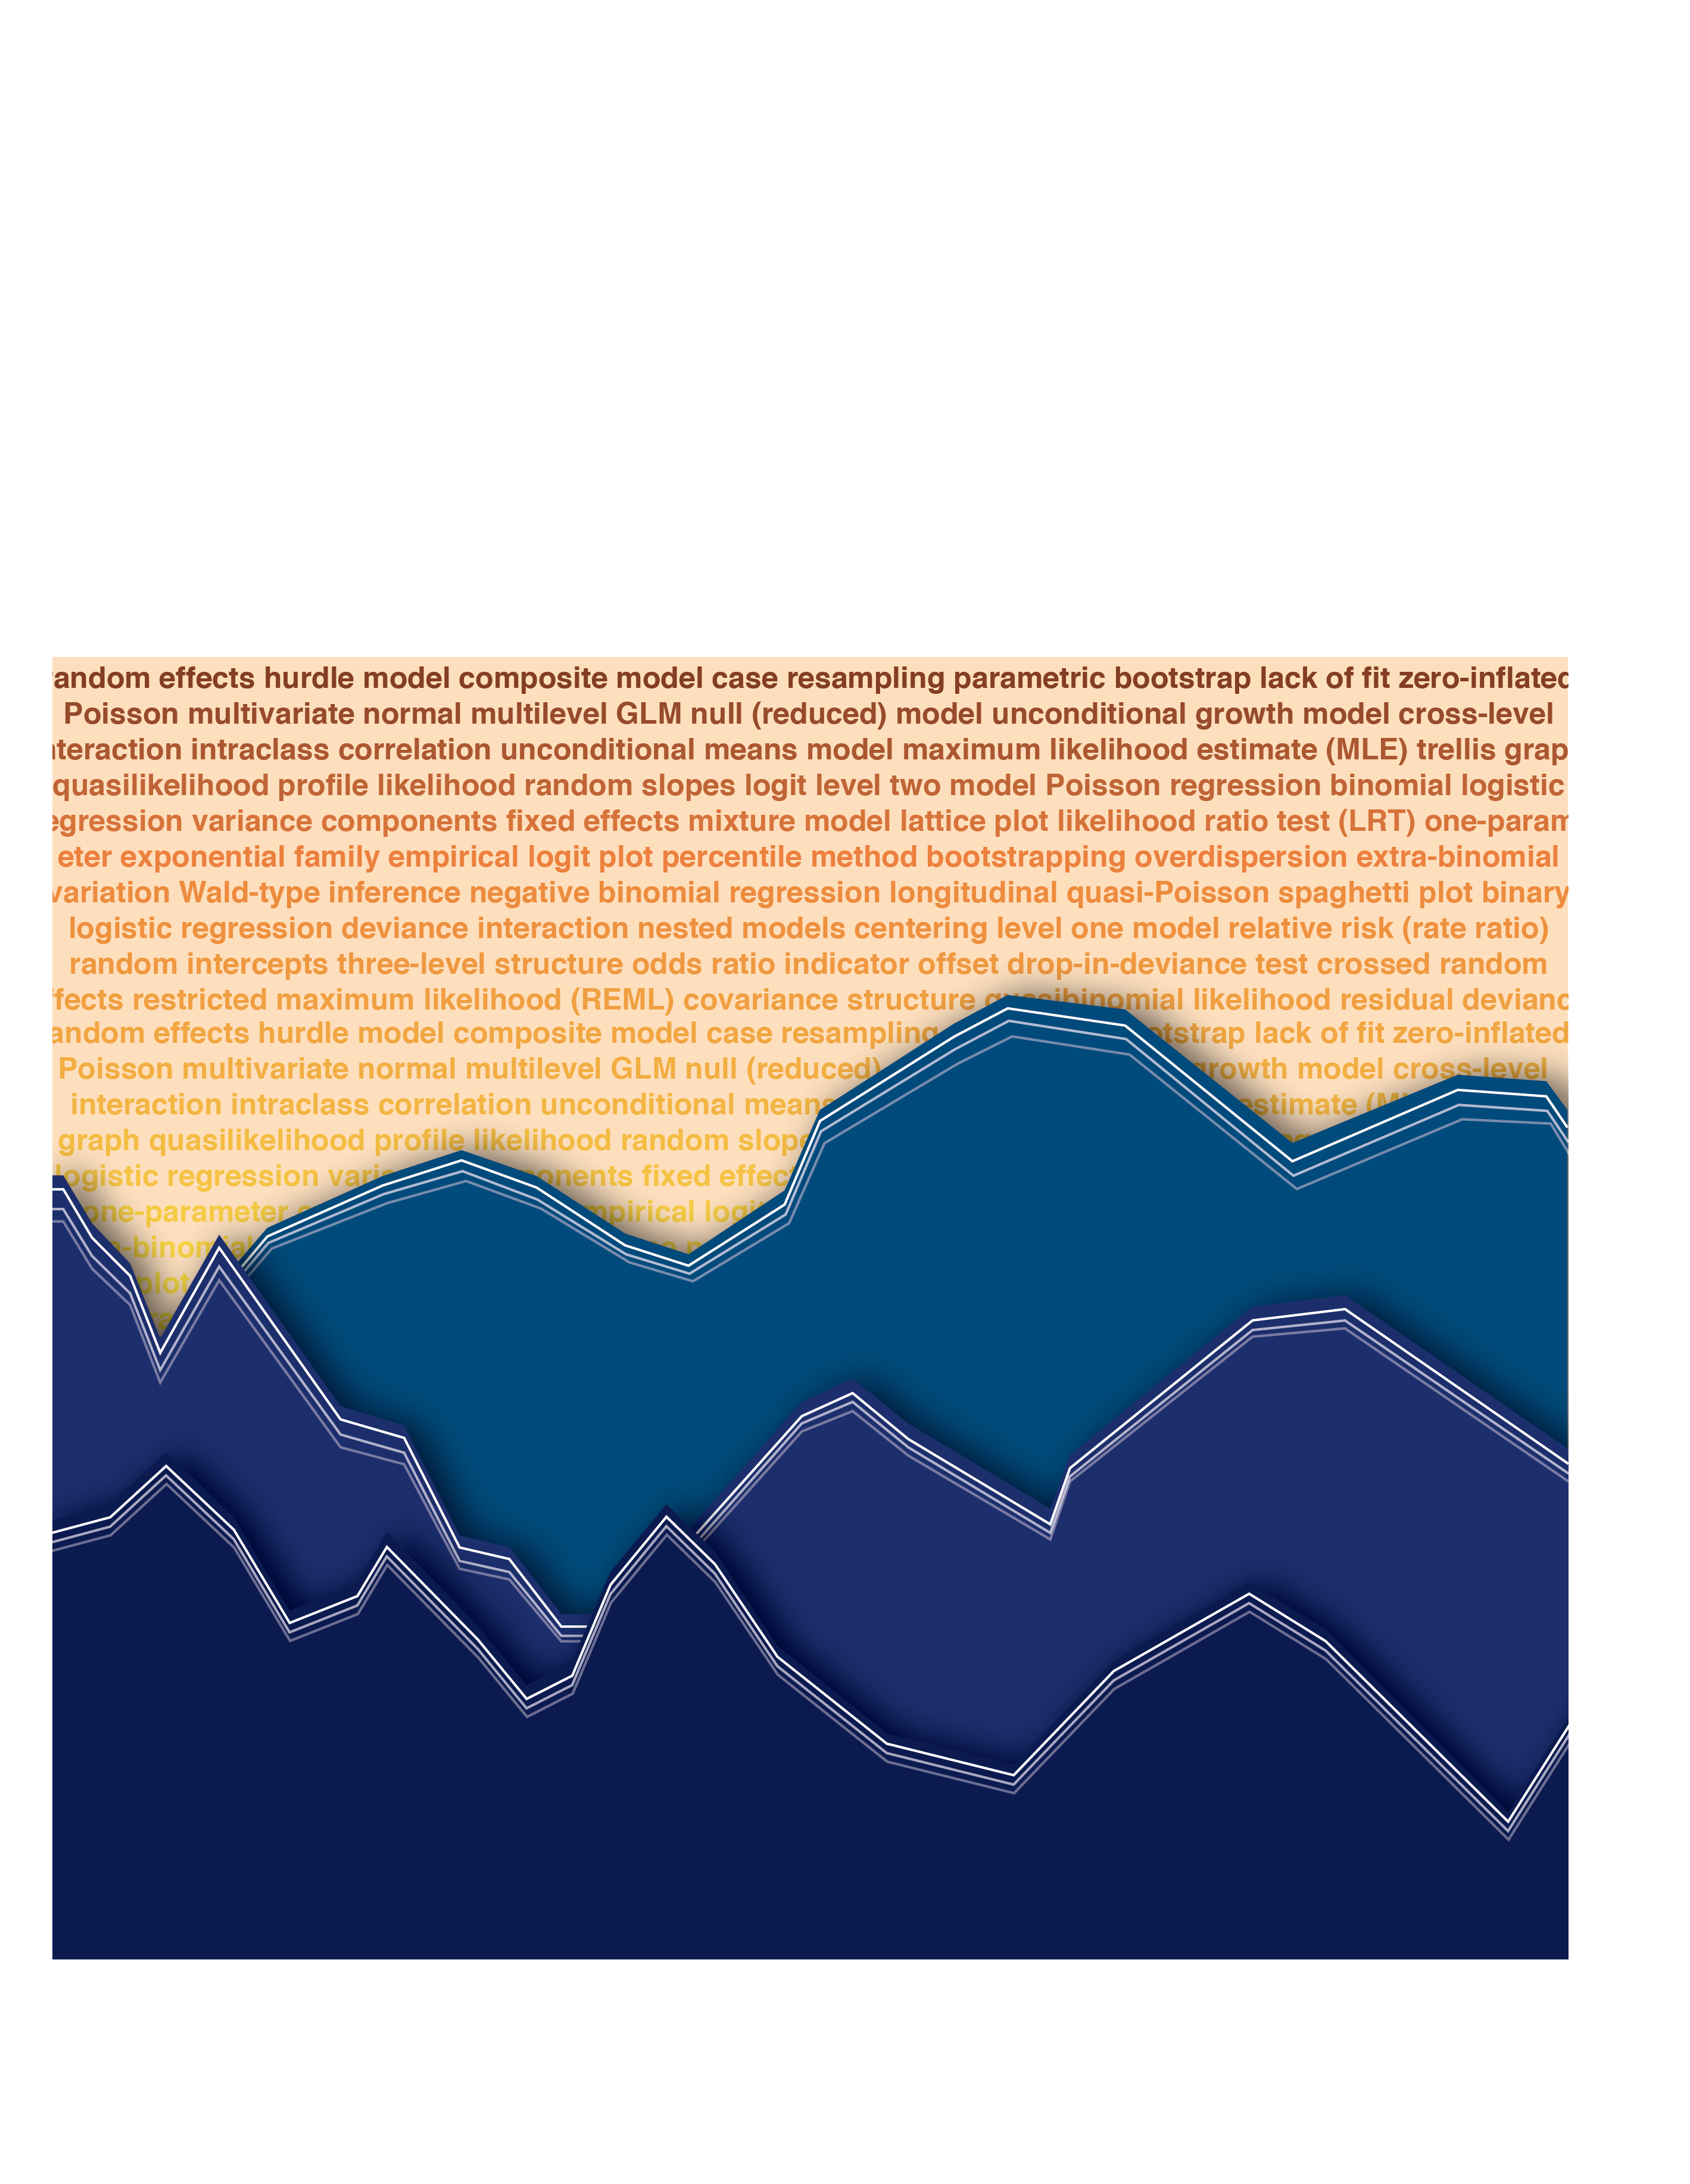
\includegraphics[width=0.75\linewidth]{data/cover}

\textbf{GLMs and Multilevel Models: Broadening Your Statistical Horizons (BYSH) with Applications using R} \citet{RProject} is intended to be accessible to undergraduate students who have successfully completed a regression course through, for example, a textbook like \emph{Stat2} \citep{Cannon2019}. We started teaching this course at St.~Olaf in 2003 so students would be able to deal with the non-normal, correlated world we live in. It has been offered at St.~Olaf every year since. Even though there is no mathematical prerequisite, we still introduce fairly sophisticated topics such as likelihood theory, zero-inflated Poisson, and parametric bootstrapping in an intuitive and applied manner. We believe strongly in case studies featuring real data and real research questions; thus, most of the data in the textbook and \href{https://github.com/proback/BYSH}{available at our GitHub repo} arises from collaborative research conducted by the authors and their students, or from student projects. Our goal is that, after working through this material, students will not necessarily be expert in these methods and associated theory, but that they will develop an expanded toolkit and a greater appreciation for the wider world of data and statistical modeling.

This work is licensed under a Creative Commons Attribution-NonCommercial-ShareAlike 4.0 International License.

\textbf{Acknowledgements.} We would like to thank students of Stat 316 at St.~Olaf College since 2010 for their patience as this book has taken shape with their feedback. We would especially like to thank these St.~Olaf students for their summer research efforts which significantly improved aspects of this book: Cecilia Noecker, Anna Johanson, Nicole Bettes, Kiegan Rice, Anna Wall, Jack Wolf, Josh Pelayo, Spencer Eanes, and Emily Patterson. Early editions of this book also benefitted greatly from feedback from instructors who used these materials in their classes, including Matt Beckman, Laura Boehm Vock, Beth Chance, Laura Chihara, Mine Dogucu, and Katie Ziegler-Graham. Finally, we have appreciated the support of two NSF grants (\#DMS-1045015 and \#DMS-0354308) and of our colleagues in Mathematics, Statistics, and Computer Science at St.~Olaf.

\hypertarget{ch-poissonreg}{%
\chapter{Poisson Regression}\label{ch-poissonreg}}

\hypertarget{learning-objectives}{%
\section{Learning Objectives}\label{learning-objectives}}

After finishing this chapter, you should be able to:

\begin{itemize}
\tightlist
\item
  Describe why simple linear regression is not ideal for Poisson data.
\item
  Write out a Poisson regression model and identify the assumptions for inference.
\item
  Write out the likelihood for a Poisson regression and describe how it could be used to estimate coefficients for a model.
\item
  Interpret estimated coefficients from a Poisson regression and construct confidence intervals for them.
\item
  Use deviances for Poisson regression models to compare and assess models.
\item
  Use an offset to account for varying effort in data collection.
\item
  Fit and use a zero-inflated Poisson (ZIP) model.
\end{itemize}

\begin{Shaded}
\begin{Highlighting}[]
\CommentTok{# Packages required for Chapter 4}
\KeywordTok{library}\NormalTok{(gridExtra)}
\KeywordTok{library}\NormalTok{(knitr)}
\KeywordTok{library}\NormalTok{(kableExtra)}
\KeywordTok{library}\NormalTok{(mosaic)}
\KeywordTok{library}\NormalTok{(xtable)}
\KeywordTok{library}\NormalTok{(pscl) }
\KeywordTok{library}\NormalTok{(multcomp)}
\KeywordTok{library}\NormalTok{(pander)}
\KeywordTok{library}\NormalTok{(MASS)}
\KeywordTok{library}\NormalTok{(tidyverse)}
\end{Highlighting}
\end{Shaded}

\hypertarget{introduction-to-poisson-regression}{%
\section{Introduction to Poisson Regression}\label{introduction-to-poisson-regression}}

Consider the following questions:

\begin{enumerate}
\def\labelenumi{\arabic{enumi}.}
\tightlist
\item
  Are the number of motorcycle deaths in a given year related to a state's helmet laws?
\item
  Does the number of employers conducting on-campus interviews during a year differ for public and private colleges?
\item
  Does the daily number of asthma-related visits to an Emergency Room differ depending on air pollution indices?
\item
  Has the number of deformed fish in randomly selected Minnesota lakes been affected by changes in trace minerals in the water over the last decade?
\end{enumerate}

Each example involves predicting a response using one or more explanatory variables, although these examples have response variables that are counts per some unit of time or space. A Poisson random variable is often used to model counts; see Chapter \ref{ch-distthry} for properties of the Poisson distribution. Since a Poisson random variable is a count, its minimum value is zero and, in theory, the maximum is unbounded. We'd like to model our main parameter \(\lambda\), the average number of occurrences per unit of time or space, as a function of one or more covariates. For example, in the first question above, \(\lambda_i\) represents the average number of motorcycle deaths in a year for state \(i\), and we hope to show that state-to-state variability in \(\lambda_i\) can be explained by state helmet laws.

For a linear least squares regression model, the parameter of interest is the average response, \(\mu_i\), for subject \(i\), and \(\mu_i\) is modeled as a line in the case of one explanatory variable. By analogy, it might seem reasonable to try to model the Poisson parameter \(\lambda_i\) as a linear function of an explanatory variable, but there are some problems with this approach. In fact, a model like \(\lambda_i=\beta_0+\beta_1x_i\) doesn't work well for Poisson data. A line is certain to yield negative values for certain \(x_i\), but \(\lambda_i\) can only take on values from 0 to \(\infty\). In addition, the equal variance assumption in linear regression inference is violated because as the mean rate for a Poisson variable increases the variance also increases (recall from Chapter \ref{ch-distthry} that if \(Y\) is the observed count, then \(E(Y)=Var(Y)=\lambda\)).

One way to avoid these problems is to model log(\(\lambda_i\)) instead of \(\lambda_i\) as a function of the covariates. The log(\(\lambda_i\)) takes on values from \(-\infty\) to \(\infty\). We can also take into account the increase in the variance with an increasing mean using this approach. (Note that throughout \emph{Broadening Your Statistical Horizons} we use log to represent the natural logarithm.) Thus, we will consider the \textbf{Poisson regression} \index{Poisson regression} model:

\begin{equation*}
log(\lambda_i)=\beta_0+\beta_1 x_i
\end{equation*}
where the observed values \(Y_i \sim\) Poisson with \(\lambda=\lambda_i\) for a given \(x_i\). For example, each state \(i\) can potentially have a different \(\lambda\) depending on its value of \(x_i\), where \(x_i\) could represent presence or absence of a particular helmet law. Note that the Poisson regression model contains no separate error term like the \(\epsilon\) we see in linear regression, because \(\lambda\) determines both the mean and the variance of a Poisson random variable.

\hypertarget{poisson-regression-assumptions}{%
\subsection{Poisson Regression Assumptions}\label{poisson-regression-assumptions}}

Much like linear least squares regression (LLSR), using Poisson regression to make inferences requires model assumptions.

\begin{enumerate}
\def\labelenumi{\arabic{enumi}.}
\tightlist
\item
  \textbf{Poisson Response} The response variable is a count per unit of time or space, described by a Poisson distribution.
\item
  \textbf{Independence} The observations must be independent of one another.
\item
  \textbf{Mean=Variance} By definition, the mean of a Poisson random variable must be equal to its variance.
\item
  \textbf{Linearity} The log of the mean rate, log(\(\lambda\)), must be a linear function of x.
\end{enumerate}

\hypertarget{a-graphical-look-at-poisson-regression}{%
\subsection{A Graphical Look at Poisson Regression}\label{a-graphical-look-at-poisson-regression}}

\begin{figure}

{\centering 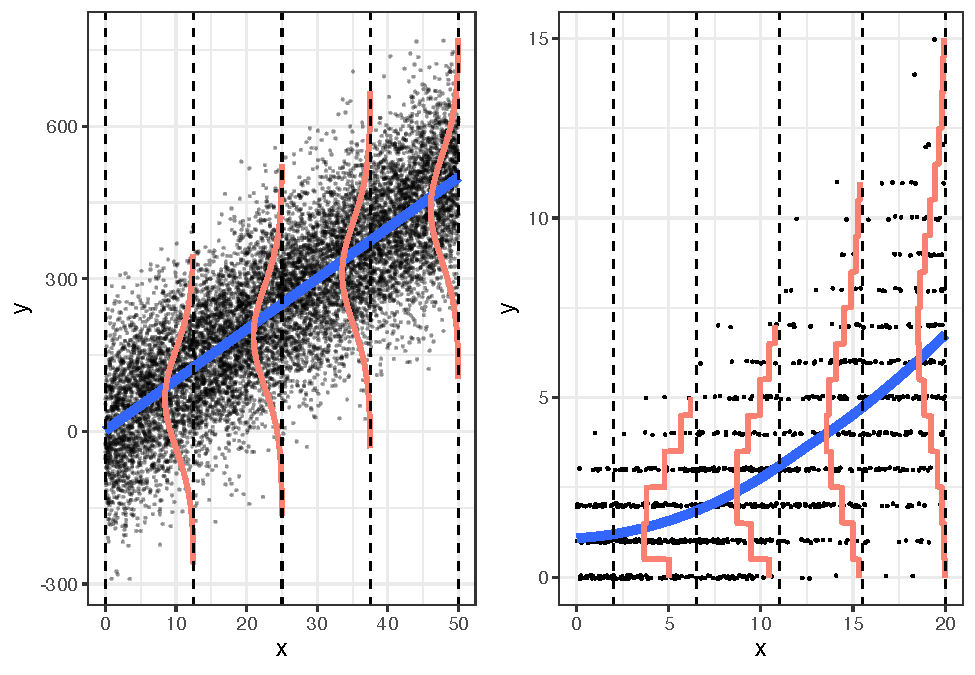
\includegraphics[width=0.6\linewidth]{bookdown-bysh_files/figure-latex/OLSpois-1} 

}

\caption{Regession Models: Linear Regression (left) and Poisson Regression (right)}\label{fig:OLSpois}
\end{figure}

Figure \ref{fig:OLSpois} illustrates a comparison of the LLSR model for inference to Poisson regression using a log function of \(\lambda\).

\begin{enumerate}
\def\labelenumi{\arabic{enumi}.}
\tightlist
\item
  The graphic displaying the linear least squares regression (LLSR) inferential model appears in the left panel of Figure \ref{fig:OLSpois}. It shows that, for each level of X, the responses are approximately normal. The panel on the right side of Figure \ref{fig:OLSpois} depicts what a Poisson regression model looks like. For each level of X, the responses follow a Poisson distribution (Assumption 1). For Poisson regression, small values of \(\lambda\) are associated with a distribution that is noticeably skewed with lots of small values and only a few larger ones. As \(\lambda\) increases the distribution of the responses begins to look more and more like a normal distribution.
\item
  In the LLSR model, the variation in \(Y\) at each level of X, \(\sigma^2\), is the same. For Poisson regression the responses at each level of X become more variable with increasing means, where variance=mean (Assumption 3).
\item
  In the case of LLSR, the mean responses for each level of X, \(\mu_{Y|X}\), fall on a line. In the case of the Poisson model, the mean values of \(Y\) at each level of \(X\), \(\lambda_{Y|X}\), fall on a curve, not a line, although the logs of the means should follow a line (Assumption 4).
\end{enumerate}

\hypertarget{case-studies-overview}{%
\section{Case Studies Overview}\label{case-studies-overview}}

We take a look at the Poisson regression model in the context of three case studies. Each case study is based on real data and real questions. Modeling household size in the Philippines introduces the idea of regression with a Poisson response along with its assumptions. A quadratic term is added to a model to determine an optimal size per household, and methods of model comparison are introduced. The campus crime case study introduces two big ideas in Poisson regression modeling: offsets, to account for sampling effort, and overdispersion, when actual variability exceeds what is expected by the model. Finally, the weekend drinking example uses a modification of a Poisson model to account for more zeros than would be expected for a Poisson random variable. These three case studies also provide context for some of the familiar concepts related to modeling such as exploratory data analysis, estimation, and residual plots.

\hypertarget{cs-philippines}{%
\section{Case Study: Household Size in the Philippines}\label{cs-philippines}}

How many other people live with you in your home? The number of people sharing a house differs from country to country and often from region to region. International agencies use household size when determining needs of populations, and the household sizes determine the magnitude of the household needs.

The Philippine Statistics Authority (PSA) spearheads the Family Income and Expenditure Survey (FIES) nationwide. The survey, which is undertaken every three years, is aimed at providing data on family income and expenditure, including levels of consumption by item of expenditure. Our data, from the 2015 FIES, is a subset of 1500 of the 40,000 observations \citep{PSA}. Our dataset focuses on five regions: Central Luzon, Metro Manila, Ilocos, Davao, and Visayas (see Figure \ref{fig:philippinesmap}).

\begin{figure}
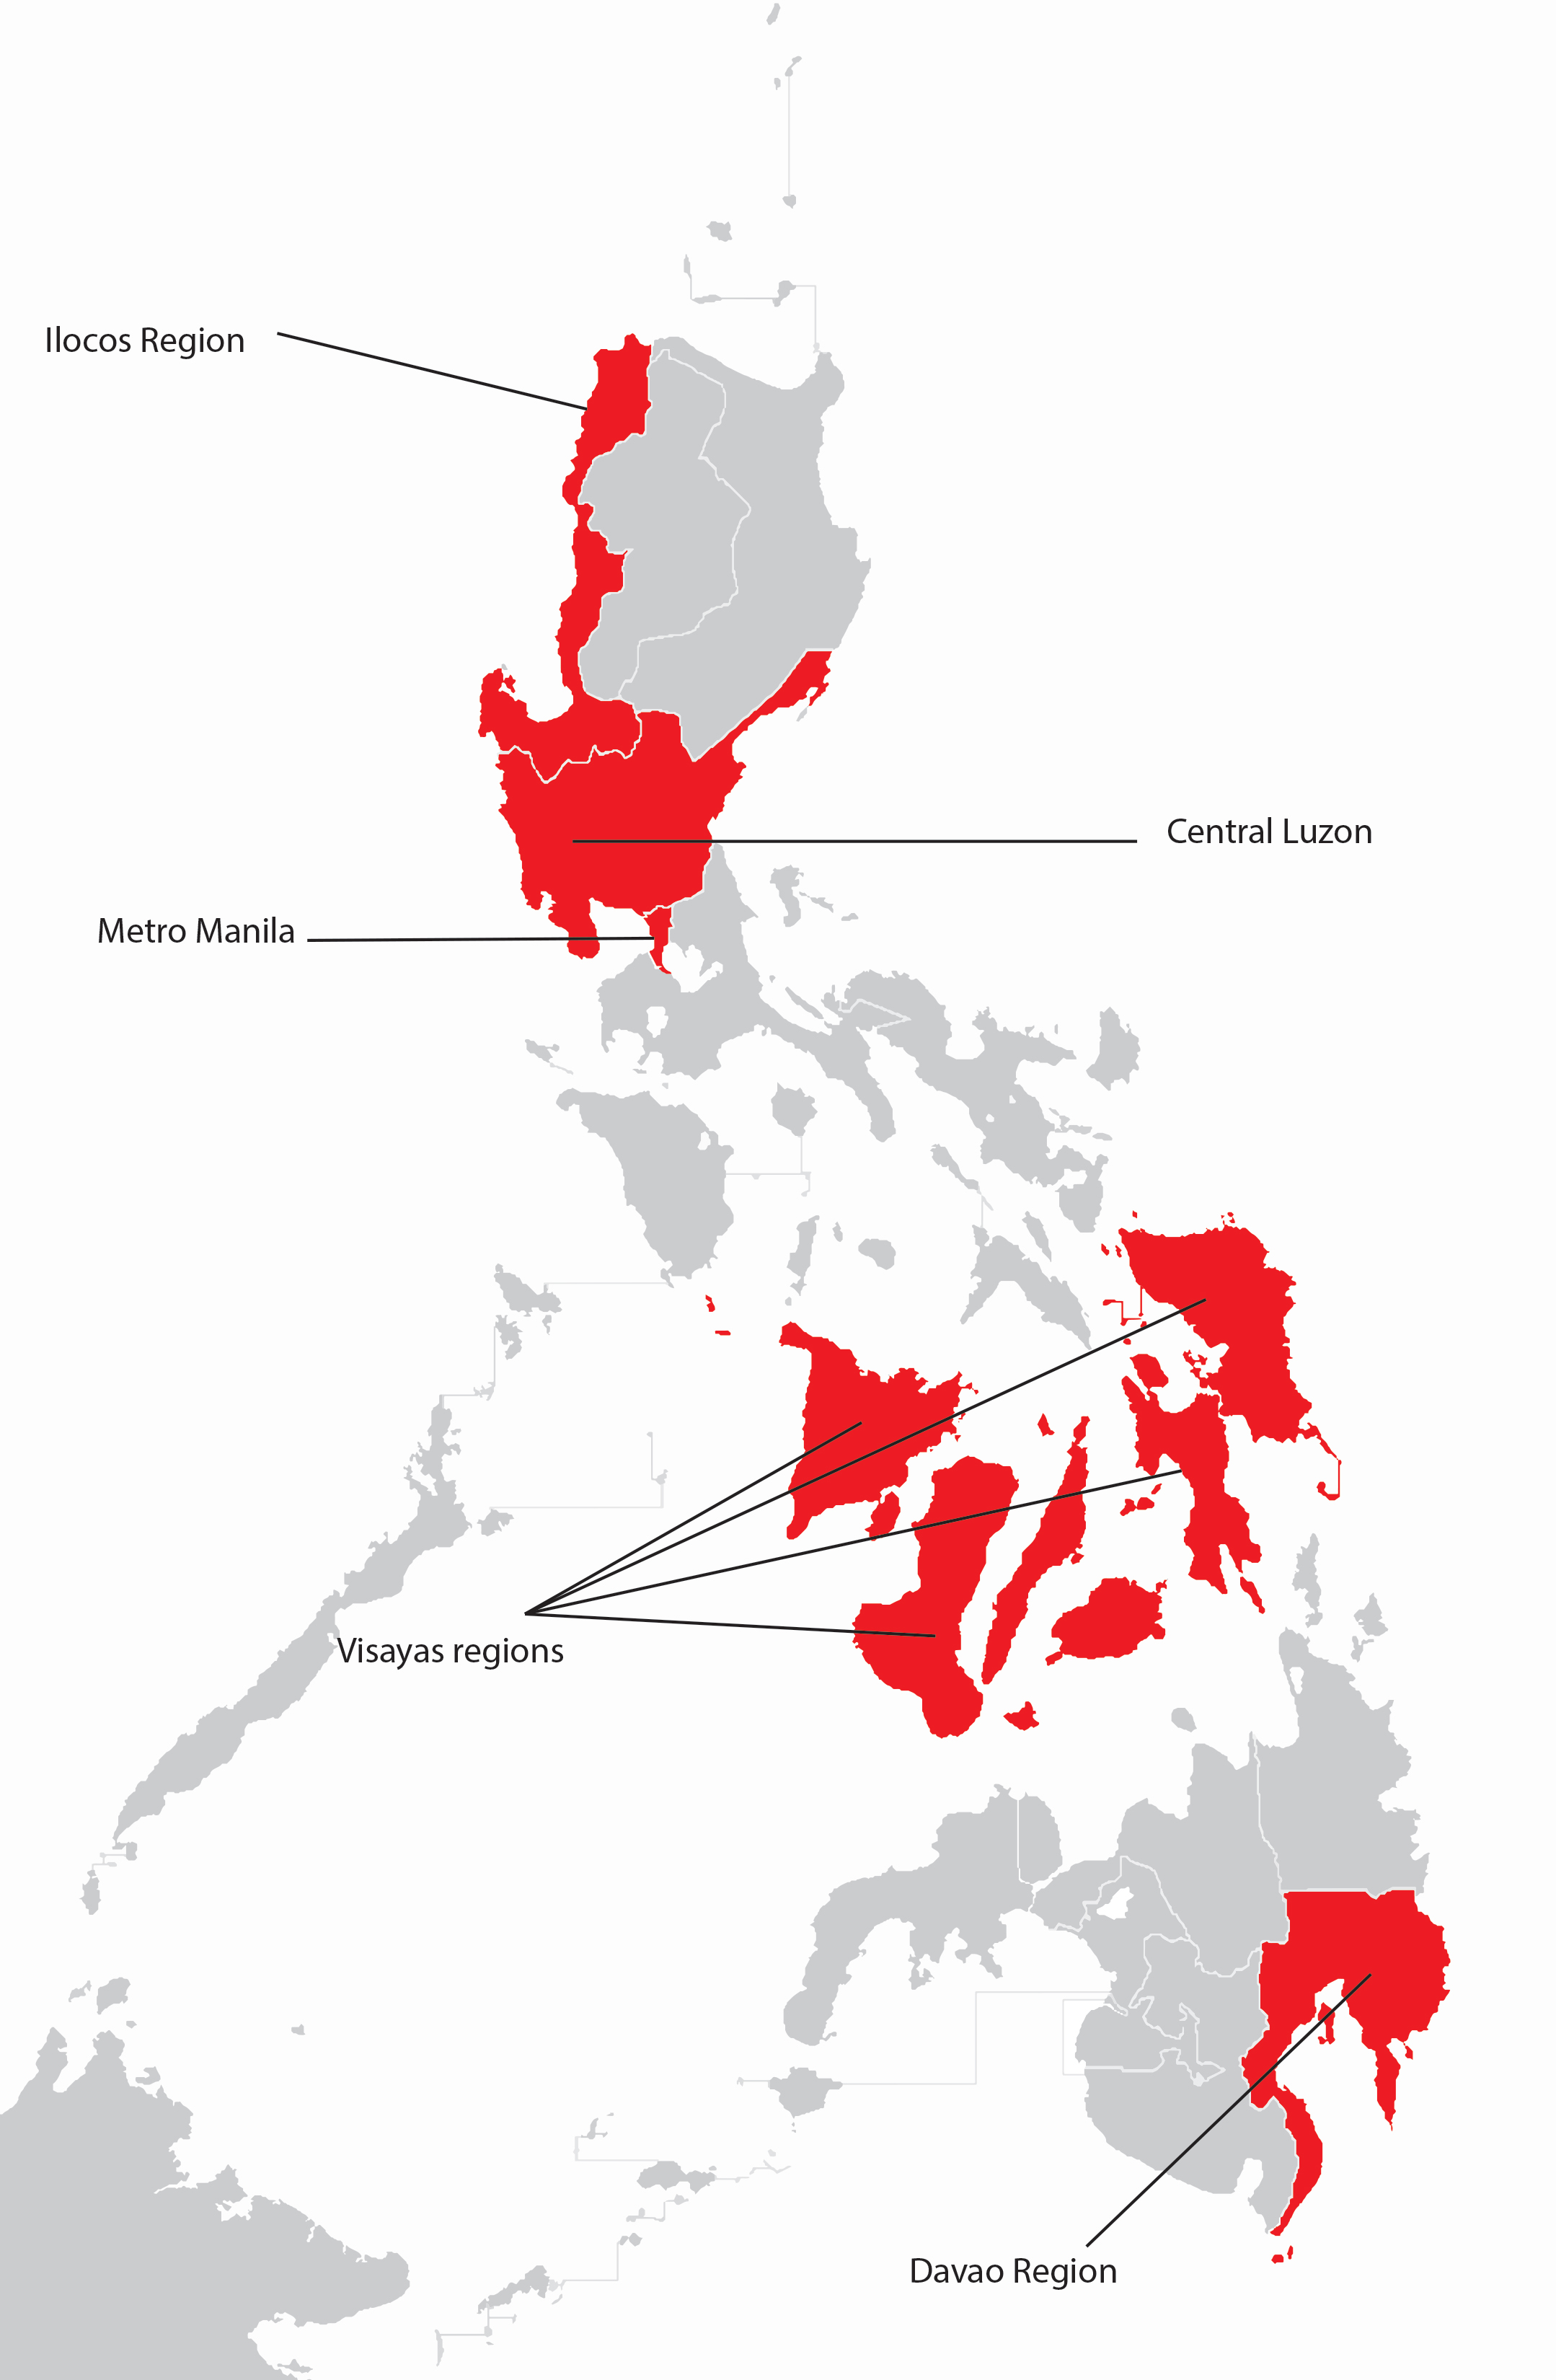
\includegraphics[width=0.5\linewidth]{data/map_of_philippines} \caption{Regions of the Philippines}\label{fig:philippinesmap}
\end{figure}

At what age are heads of households in the Philippines most likely to find the largest number of people in their household? Is this association similar for poorer households (measured by the presence of a roof made from predominantly light/salvaged materials)? We begin by explicitly defining our response, \(Y=\) number of household members other than the head of the household. We then define the explanatory variables: age of the head of the household, type of roof (predominantly light/salvaged material or predominantly strong material), and location (Central Luzon, Davao Region, Ilocos Region, Metro Manila, or Visayas). Note that predominantly light/salvaged materials are a combination of light material, mixed but predominantly light material, and mixed but predominantly salvaged material, and salvaged matrial. Our response is a count, so we consider a Poisson regression where the parameter of interest is \(\lambda\), the average number of people, other than the head, per household. We will primarily examine the relationship between household size and age of the head of household, controlling for location and income.

\hypertarget{organizedata4}{%
\subsection{Data Organization}\label{organizedata4}}

The first five rows from our data set \texttt{fHH1.csv} are illustrated in Table \ref{tab:fHH1table1}. Each line of the data file refers to a household at the time of the survey:

\begin{itemize}
\tightlist
\item
  \texttt{location} = where the house is located (Central Luzon, Davao Region, Ilocos Region, Metro Manila, or Visayas)
\item
  \texttt{age} = the age of the head of household
\item
  \texttt{total} = the number of people in the household other than the head
\item
  \texttt{numLT5} = the number in the household under 5 years of age
\item
  \texttt{roof} = the type of roof in the household (either Predominantly Light/Salvaged Material, or Predominantly Strong Material, where stronger material can sometimes be used as a proxy for greater wealth)
\end{itemize}

\begin{table}

\caption{\label{tab:fHH1table1}The first five observations from the Philippines Household case study.}
\centering
\begin{tabular}[t]{rlrrrl}
\toprule
X1 & location & age & total & numLT5 & roof\\
\midrule
1 & CentralLuzon & 65 & 0 & 0 & Predominantly Strong Material\\
2 & MetroManila & 75 & 3 & 0 & Predominantly Strong Material\\
3 & DavaoRegion & 54 & 4 & 0 & Predominantly Strong Material\\
4 & Visayas & 49 & 3 & 0 & Predominantly Strong Material\\
5 & MetroManila & 74 & 3 & 0 & Predominantly Strong Material\\
\bottomrule
\end{tabular}
\end{table}

\hypertarget{exploreHH}{%
\subsection{Exploratory Data Analyses}\label{exploreHH}}

For the rest of this case study, we will refer to the number of people in a household as the total number of people in that specific household \emph{besides} the head of household. The average number of people in a household is 3.68 (Var = 5.53), and there are anywhere from 0 to 16 people in the houses. Over 11.1\% of these households are made from predominantly light and salvaged material. The mean number of people in a house for houses with a roof made from predominantly strong material is is 3.69 (Var=5.55), whereas houses with a roof made from predominantly light/salvaged material average 3.64 people (Var=5.41). Of the various locations, Visayas has the largest household size, on average, with a mean of 3.90 in the household, and the Davao Region has the smallest with a mean of 3.39.

\begin{figure}

{\centering 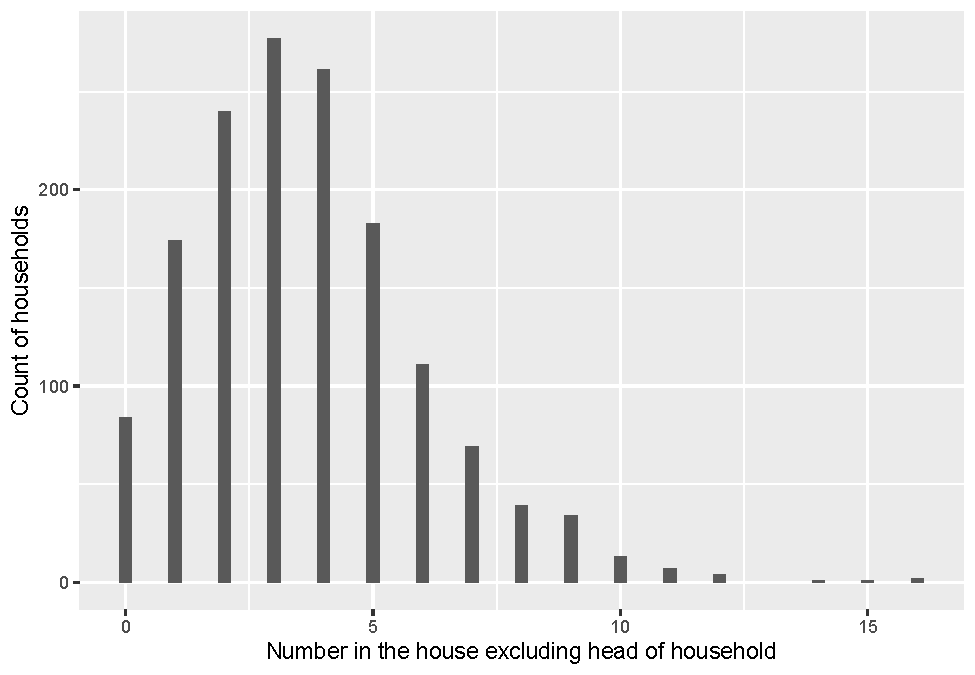
\includegraphics[width=0.6\linewidth]{bookdown-bysh_files/figure-latex/nhouse-1} 

}

\caption{Distribution of household size in 5 Philippine regions}\label{fig:nhouse}
\end{figure}

Figure \ref{fig:nhouse} reveals a fair amount of variability in the number in each house; responses range from 0 to 16 with many of the respondents reporting between 1 and 5 people in the house. Like many Poisson distributions, this graph is right skewed. It clearly does not suggest that the number of people in a household is a normally distributed response.

\begin{figure}

{\centering 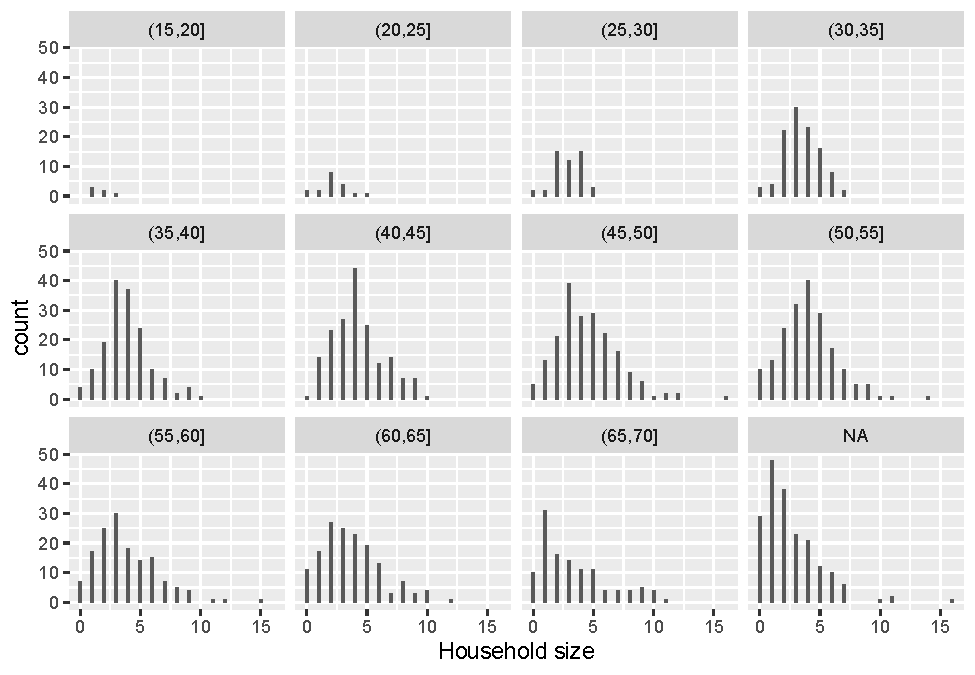
\includegraphics[width=0.6\linewidth]{bookdown-bysh_files/figure-latex/totalPoisByAge-1} 

}

\caption{Distribution of household sizes by age group of the household head.}\label{fig:totalPoisByAge}
\end{figure}

Figure \ref{fig:totalPoisByAge} further shows that responses can be reasonably modeled with a Poisson distribution when grouped by a key explanatory variable: age of the household head. These last two plots together suggest that Assumption 1 (Poisson Response) is satisfactory in this case study.

For Poisson random variables, the variance of \(Y\) (i.e., the square of the standard deviation of \(Y\)), is equal to its mean, where \(Y\) represents the size of an individual household. As the mean increases, the variance increases. So, if the response is a count and the mean and variance are approximately equal for each group of \(X\), a Poisson regression model may be a good choice. In Table \ref{tab:table1chp4} we display age groups by 5-year increments, to check to see if the empirical means and variances of the number in the house are approximately equal for each age group. This provides us one way in which to check the Poisson Assumption 3 (mean = variance).

\begin{table}

\caption{\label{tab:table1chp4}Compare mean and variance of household size within each age group}
\centering
\begin{tabular}[t]{lrrr}
\toprule
Age Groups & Mean & Variance & n\\
\midrule
(15,20] & 1.667 & 0.6667 & 6\\
(20,25] & 2.167 & 1.5588 & 18\\
(25,30] & 2.918 & 1.4099 & 49\\
(30,35] & 3.444 & 2.1931 & 108\\
(35,40] & 3.842 & 3.5735 & 158\\
\addlinespace
(40,45] & 4.234 & 4.4448 & 175\\
(45,50] & 4.490 & 6.3963 & 194\\
(50,55] & 4.011 & 5.2512 & 188\\
(55,60] & 3.807 & 6.5319 & 145\\
(60,65] & 3.706 & 6.1958 & 153\\
\addlinespace
(65,70] & 3.339 & 7.9980 & 115\\
NA & 2.550 & 5.5436 & 191\\
\bottomrule
\end{tabular}
\end{table}

If there is a problem with this assumption, most often we see variances much larger than means. Here, as expected, we see more variability as age increases. However, it appears that the variance is smaller than the mean for lower ages, while the variance is greater than the mean for higher ages. Thus, there is some evidence of a violation of the mean=variance assumption (Assumption 3), although any violations are modest.

The Poisson regression model also implies that log(\(\lambda_i\)), not the mean household size \(\lambda_i\), is a linear function of age; i.e., \(log(\lambda_i)=\beta_0+\beta_1\textrm{age}_i\). Therefore, to check the linearity assumption (Assumption 4) for Poisson regression we would like to plot log(\(\lambda_i\)) by age. Unfortunately, \(\lambda_i\) is unknown. Our best guess of \(\lambda_i\) is the observed mean number in the household for each age (level of \(X\)). Because these means are computed for observed data, they are referred to as \textbf{empirical} means. Taking the logs of the empirical means and plotting by age provides a way to assess the linearity assumption. The smoothed curve added to Figure \ref{fig:ageXnhouse} suggests that there is a curvilinear relationship between age and the log of the mean household size, implying that adding a quadratic term should be considered. This finding is consistent with the researchers' hypothesis that there is an age at which a maximum household size occurs. It is worth noting that we are not modeling the log of the empirical means, rather it is the log of the \emph{true} rate that is modeled. Looking at empirical means, however, does provide an idea of the form of the relationship between log(\(\lambda)\) and \(x_i\).

\begin{figure}

{\centering 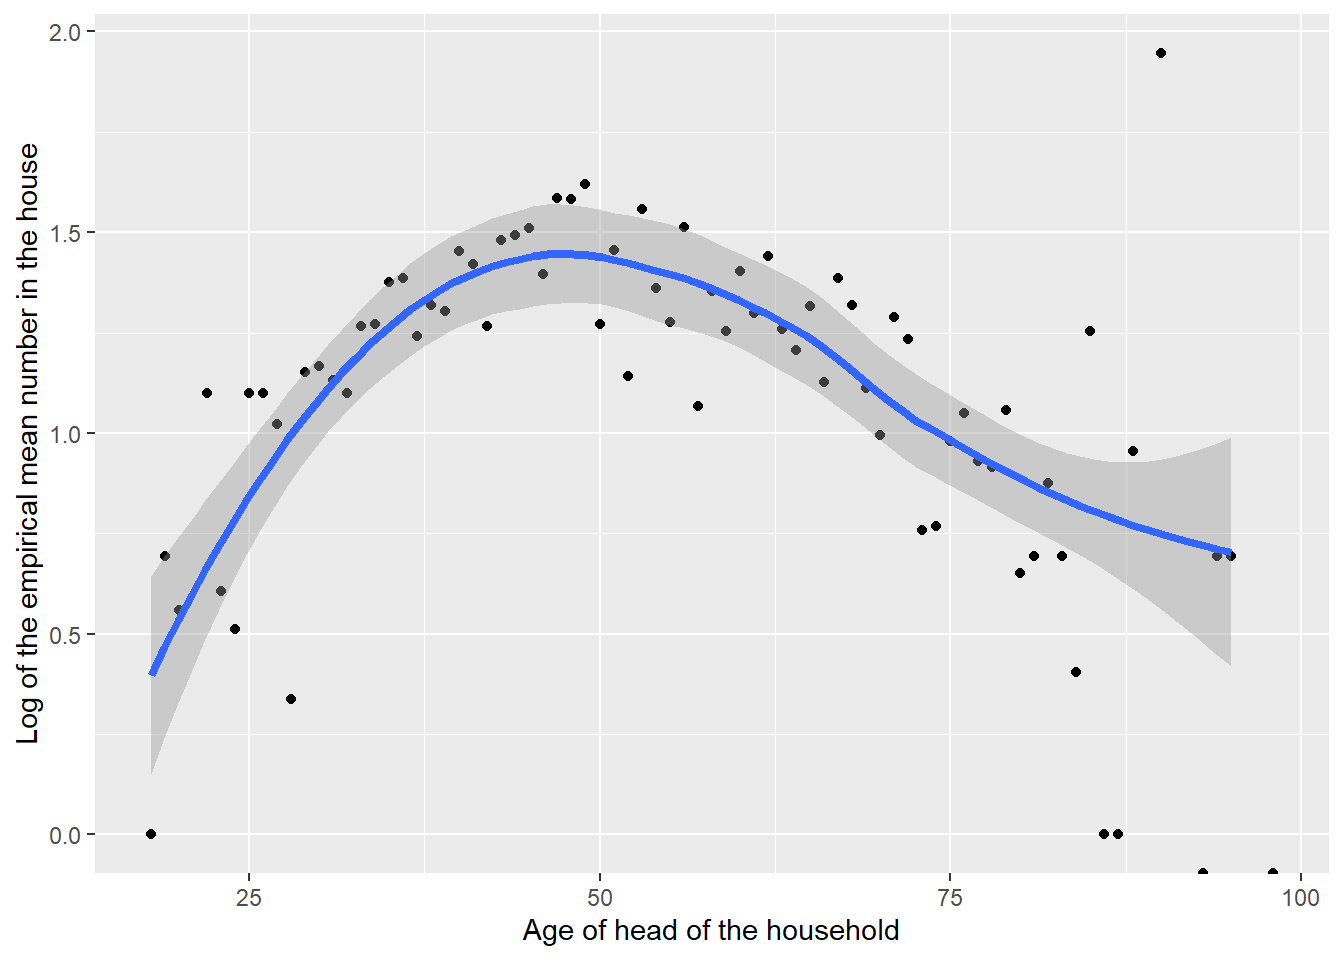
\includegraphics[width=0.6\linewidth]{bookdown-bysh_files/figure-latex/ageXnhouse-1} 

}

\caption{The log of the mean household sizes, besides the head of household, by age of the head of household, with loess smoother.}\label{fig:ageXnhouse}
\end{figure}

We can extend Figure \ref{fig:ageXnhouse} by fitting separate curves for each region (see Figure \ref{fig:byregion}). This allows us to see if the relationship between mean household size and age is consistent across region. In this case, the relationships are pretty similar; if they weren't we could consider adding an age-by-region interaction to our eventual Poisson regression model.

\begin{figure}

{\centering 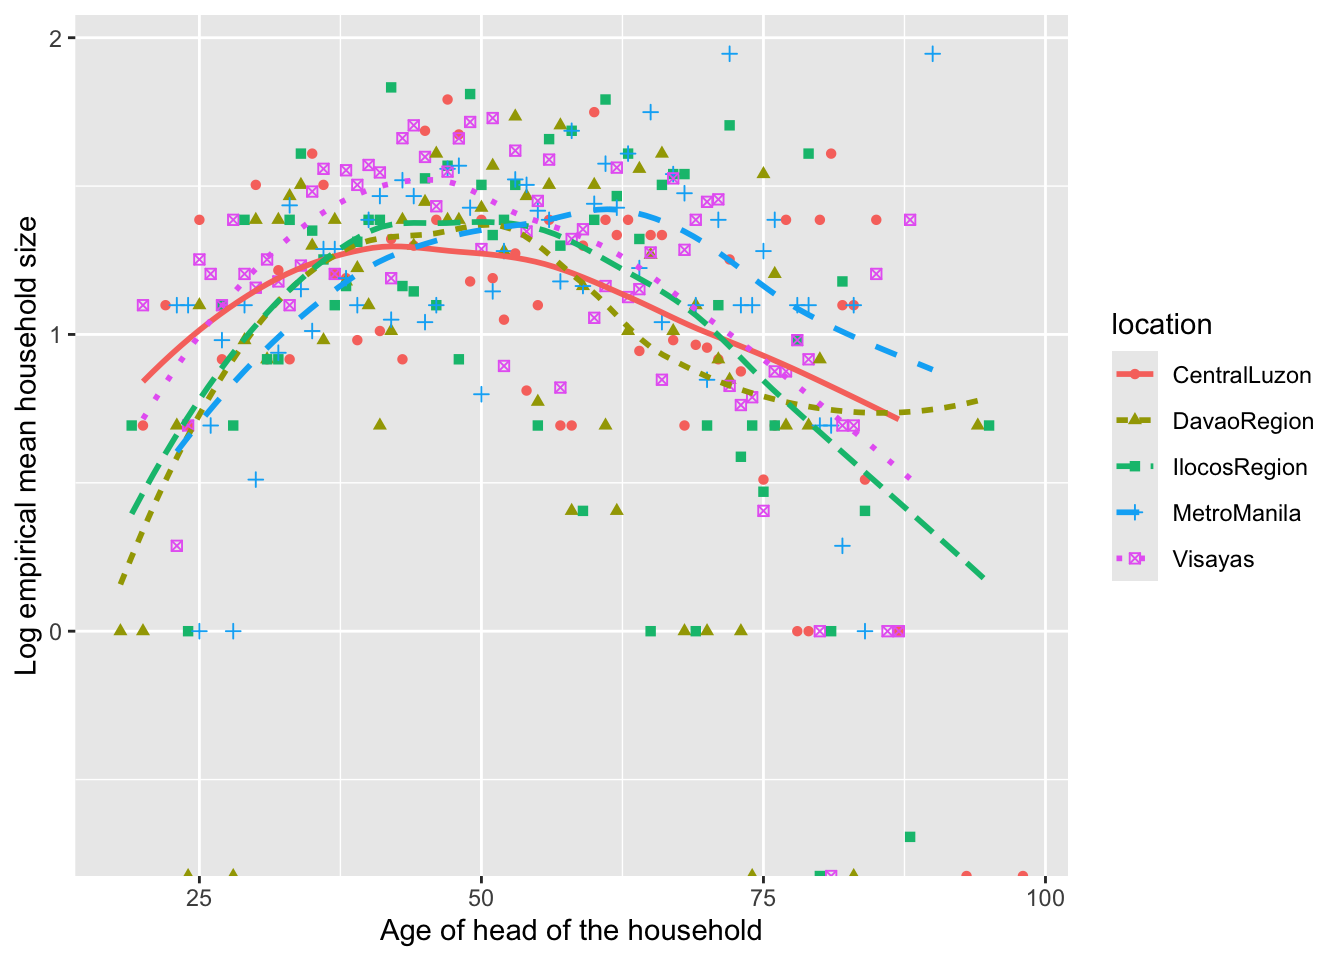
\includegraphics[width=0.6\linewidth]{bookdown-bysh_files/figure-latex/byregion-1} 

}

\caption{Empirical log of the mean household sizes vs. age of the head of household, with loess smoother by region.}\label{fig:byregion}
\end{figure}

Finally, the independence assumption (Assumption 2) can be assessed using knowledge of the study design and the data collection process. In this case, we do not have enough information to assess the independence assumption with the information we are given. If each household was not selected individually in a random manner, but rather groups of households were selected from different regions with differing customs about living arrangements, the independence assumption would be violated. If this were the case, we could use a multilevel model like those discussed in later chapters with a village term.

\hypertarget{sec-PoisInference}{%
\subsection{Estimation and Inference}\label{sec-PoisInference}}

We first consider a model for which log(\(\lambda\)) is linear in age. We then will determine whether a model with a quadratic term in age provides a significant improvement based on trends we observed in the exploratory data analysis.

R reports an estimated regression equation for the linear Poisson model as:

\begin{equation*}
log(\hat{\lambda}) = 1.55 - 0.0047 \textrm{age}
\end{equation*}

\begin{Shaded}
\begin{Highlighting}[]
\NormalTok{modela =}\StringTok{ }\KeywordTok{glm}\NormalTok{(total }\OperatorTok{~}\StringTok{ }\NormalTok{age, }\DataTypeTok{family =}\NormalTok{ poisson, }\DataTypeTok{data =}\NormalTok{ fHH1)}
\end{Highlighting}
\end{Shaded}

\begin{verbatim}
##              Estimate Std. Error z value   Pr(>|z|)
## (Intercept)  1.549942  0.0502754  30.829 1.070e-208
## age         -0.004706  0.0009363  -5.026  5.013e-07
\end{verbatim}

\begin{verbatim}
##  Residual deviance =  2337  on  1498 df 
##  Dispersion parameter =  1
\end{verbatim}

How can the coefficient estimates be interpreted in terms of this example? As done when interpreting slopes in the LLSR models, we consider how the estimated mean number in the house, \(\lambda\), changes as the age of the household head increases by an additional year. But in place of looking at change in the mean number in the house, with a Poisson regression we consider the log of the mean number in the house and then convert back to original units. For example, consider a comparison of two models---one for a given age (\(x\)) and one after increasing age by 1 (\(x+1\))

\begin{equation}
\begin{split}
log(\lambda_X) &= \beta_0 + \beta_1X \\
log(\lambda_{X+1}) &= \beta_0 + \beta_1(X+1) \\
log(\lambda_{X+1})-log(\lambda_X) &=  \beta_1 \\
log \left(\frac{\lambda_{X+1}}{\lambda_X}\right)   &= \beta_1\\
\frac{\lambda_{X+1}}{\lambda_X} &= e^{\beta_1}
\end{split}
\label{eq:rateRatio}
\end{equation}

These results suggest that by exponentiating the coefficient on age we obtain the multiplicative factor by which the mean count changes. In this case, the mean number in the house changes by a factor of \(e^{-0.0047}=0.995\) or decreases by 0.5\% (since \(1-.995 = .005\)) with each additional year older the household head is; or, we predict a 0.47\% \emph{increase} in mean household size for a 1 year \emph{decrease} in age of the household head (since \(1/.995=1.0047\)). The quantity on the left hand side of Equation \eqref{eq:rateRatio} is referred to as a \textbf{rate ratio} or \textbf{relative risk} \index{relative risk (rate ratio)}, and it represents a percent change in the response for a unit change in X. In fact, for regression models in general, whenever a variable (response or explanatory) is logged, we make interpretations about multiplicative effects on that variable, while with unlogged variables we can reach our usual interpretations about additive effects.

Typically the standard errors for the estimated coefficients are included in Poisson regression output. Here the standard error for the estimated coefficient for age is 0.00094. We can use the standard error to construct a confidence interval for \(\beta_1\). A 95\% CI provides a range of plausible values for the \texttt{age} coefficient and can be constructed:

\[(\hat\beta_1-Z^*\cdot SE(\hat\beta_1), \quad \hat\beta_1+Z^*\cdot SE(\hat\beta_1))\]
\[(-0.0047-1.96*0.00094, \quad -0.0047+1.96*0.00094)\]
\[ (-0.0065, -0.0029).
 \]

Exponentiating the endpoints yields a confidence interval for the relative risk; i.e., the percent change in household size for each additional year older. Thus \((e^{-0.0065},e^{-0.0029})=(0.993,0.997)\) suggests that we are 95\% confident that the mean number in the house decreases between 0.7\% and 0.3\% for each additional year older the head of household is. It is best to construct a confidence interval for the coefficient and then exponentiate the endpoints because the estimated coefficients more closely follow a normal distribution than the exponentiated coefficients. There are other approaches to constructing intervals in these circumstances, including profile likelihood, the delta method, and bootstrapping, and we will discuss some of those approaches later. In this case, for instance, the profile likelihood interval is nearly identical to the Wald-type (normal theory) confidence interval \index{Wald-type confidence interval} above.

\begin{Shaded}
\begin{Highlighting}[]
\CommentTok{# CI for betas using profile likelihood}
\KeywordTok{confint}\NormalTok{(modela)}
\end{Highlighting}
\end{Shaded}

\begin{verbatim}
##                 2.5 %    97.5 %
## (Intercept)  1.451170  1.648249
## age         -0.006543 -0.002873
\end{verbatim}

\begin{Shaded}
\begin{Highlighting}[]
\KeywordTok{exp}\NormalTok{(}\KeywordTok{confint}\NormalTok{(modela))}
\end{Highlighting}
\end{Shaded}

\begin{verbatim}
##              2.5 % 97.5 %
## (Intercept) 4.2681 5.1979
## age         0.9935 0.9971
\end{verbatim}

If there is no association between age and household size, there is no change in household size for each additional year, so \(\lambda_X\) is equal to \(\lambda_{X+1}\) and the ratio \(\lambda_{X+1}/\lambda_X\) is 1. In other words, if there is no association between age and household size, then \(\beta_1=0\) and \(e^{\beta_1}=1\). Note that our interval for \(e^{\beta_1}\), (0.993,0.997), does not include 1, so the model with age is preferred to a model without age; i.e., age is significantly associated with household size. Note that we could have similarly confirmed that our interval for \(\beta_1\) does not include 0 to show the significance of age as a predictor of household size.

Another way to test the significance of the age term is to calculate a \textbf{Wald-type statistic} \index{Wald-type test}. A Wald-type test statistic is the estimated coefficient divided by its standard error. When the true coefficient is 0, this test statistic follows a standard normal distribution for sufficiently large \(n\). The estimated coefficient associated with the linear term in age is \({\hat{\beta}_1}=-0.0047\) with standard error \(SE(\hat{\beta}_1)=0.00094\). The value for the Wald test statistic is then \(Z=\hat{\beta}_1/SE(\hat{\beta}_1)=-5.026\), where \(Z\) follows a standard normal distribution if \(\beta_1=0\). In this case, the two-sided p-value based on the standard normal distribution for testing \(H_0:\beta_1=0\) is almost 0 (\(p=0.000000501\)). Therefore, we have statistically significant evidence (Z = -5.026, p \textless{} .001) that average household size decreases as age of the head of household increases.

\hypertarget{sec-Devtocompare}{%
\subsection{Using Deviances to Compare Models}\label{sec-Devtocompare}}

There is another way in which to assess how useful age is in our model. A \textbf{deviance} \index{deviance} is a way in which to measure how the observed data deviates from the model predictions; it will be defined more precisely in Section \ref{sec-PoisResid}, but it is similar to sum of squared errors (unexplained variability in the response) in LLSR regression. Because we want models that minimize deviance, we calculate the \textbf{drop-in-deviance} \index{drop-in-deviance test} when adding age to the model with no covariates (the \textbf{null model}) \index{null (reduced) model}. The deviances for the null model and the model with age can be found in the model output. A residual deviance for the model with age is reported as 2337.1 with 1498 df. The output also includes the deviance and degrees of freedom for the null model (2362.5 with 1499 df). The drop-in-deviance is 25.4 (2362.5 - 2337.1) with a difference of only 1 df, so that the addition of one extra term (age) reduced unexplained variability by 25.4. If the null model were true, we would expect the drop-in-deviance to follow a \(\chi^2\) distribution with 1 df. Therefore the p-value for comparing the null model to the model with age is found by determining the probability that the value for a \(\chi^2\) random variable with one degree of freedom exceeds 25.4, which is essentially 0. Once again, we can conclude that we have statistically significant evidence (\(\chi^2_{\text{df} =1}=25.4\), \(p < .001\)) that average household size decreases as age of the head of household increases.

\begin{Shaded}
\begin{Highlighting}[]
\CommentTok{# model0 is the null/reduced model}
\NormalTok{model0 <-}\StringTok{ }\KeywordTok{glm}\NormalTok{(total }\OperatorTok{~}\StringTok{ }\DecValTok{1}\NormalTok{, }\DataTypeTok{family =}\NormalTok{ poisson, }\DataTypeTok{data =}\NormalTok{ fHH1)}
\NormalTok{drop_in_dev <-}\StringTok{ }\KeywordTok{anova}\NormalTok{(model0, modela, }\DataTypeTok{test =} \StringTok{"Chisq"}\NormalTok{)}
\end{Highlighting}
\end{Shaded}

\begin{verbatim}
  ResidDF ResidDev Deviance Df      pval
1    1499     2362       NA NA        NA
2    1498     2337     25.4  1 4.661e-07
\end{verbatim}

More formally, we are testing:

\[\textrm{Null (reduced) Model}: \log(\lambda) = \beta_0 \textrm{ or } \beta_1=0\]
\[\textrm{Larger (full) Model}: \log(\lambda) = \beta_0 + \beta_1\textrm{age} \textrm{ or } \beta_1 \neq 0 \]

In order to use the drop-in-deviance test, the models being compared must be \textbf{nested} \index{nested models}; e.g., all the terms in the smaller model must appear in the larger model. Here the smaller model is the null model with the single term \(\beta_0\) and the larger model has \(\beta_0\) and \(\beta_1\), so the two models are indeed nested. For nested models, we can compare the models' residual deviances to determine whether the larger model provides a significant improvement.

Here, then, is a summary of these two approaches to hypothesis testing about terms in Poisson regression models:

\textbf{Drop-in-deviance test to compare models} \index{drop-in-deviance test}

\begin{itemize}
\tightlist
\item
  Compute the deviance for each model, then calculate: drop-in-deviance = residual deviance for reduced model - residual deviance for the larger model.
\item
  When the reduced model is true, the drop-in-deviance \(\sim \chi^2_d\)
  where d= the difference in the degrees of freedom associated with the two models (that is, the difference in the number of terms / coefficients).
\item
  A large drop-in-deviance favors the larger model.
\end{itemize}

\textbf{Wald test for a single coefficient} \index{Wald-type test}

\begin{itemize}
\tightlist
\item
  Wald-type statistic = estimated coefficient / standard error
\item
  When the true coefficient is 0, for sufficiently large \(n\), the test statistic \(\sim\) N(0,1).
\item
  If the magnitude of the test statistic is large, there is evidence that the true coefficient is not 0.
\end{itemize}

The drop-in-deviance and the Wald-type tests usually provide consistent results; however, if there is a discrepancy the drop-in-deviance is preferred. Not only does the drop-in-deviance test perform better in more cases, but it's also more flexible. If two models differ by one term, then the drop-in-deviance test essentially tests if a single coefficient is 0 like the Wald test does, while if two models differ by more than one term, the Wald test is no longer appropriate.

\hypertarget{likelihood.sec}{%
\subsection{Using Likelihoods to fit Poisson Regression Models (Optional)}\label{likelihood.sec}}

Before continuing with model building, we take a short detour to see how coefficient estimates are determined in a Poisson regression model. The least squares approach requires a linear relationship between the parameter, \(\lambda_i\) (the expected or mean response for observation \(i\)), and \(x_i\) (the age for observation \(i\)). However, it is log\((\lambda_i)\), not \(\lambda_i\), that is linearly related to X with the Poisson model. The assumptions of equal variance and normality also do not hold for Poisson regression. Thus, the method of least squares will not be helpful for inference in Poisson Regression. Instead of least squares, we employ the likelihood \index{likelihood} principle to find estimates of our model coefficients. We look for those coefficient estimates for which the likelihood of our data is maximized; these are the \textbf{maximum likelihood estimates} \index{maximum likelihood estimate (MLE)}.

The likelihood for n \emph{independent} \index{independent} observations is the product of the probabilities. For example, if we observe five households with household sizes of 4, 2, 8, 6, and 1 person beyond the head, the likelihood is:

\[ Likelihood = P(Y_1=4)*P(Y_2=2)*P(Y_3=8)*P(Y_4=6)*P(Y_5=1)\]
Recall that the probability of a Poisson response can be written

\[P(Y=y)=\frac{e^{-\lambda}\lambda^y}{y!}\]
for \(y = 0, 1, 2, ...\) So the likelihood can be written as

\begin{align*}
 Likelihood&= \frac{ e^{-\lambda_1}\lambda_1^4 }{ 4! }*
 \frac{ e^{-\lambda_2}\lambda_2^2 }{ 2! } *\frac{e^{-\lambda_3}\lambda_3^8}{8!}*
 \frac{e^{-\lambda_4}\lambda_4^6}{6!}*\frac{e^{-\lambda_5}\lambda_5^1}{1!}
 \end{align*}
where each \(\lambda_i\) can differ for each household depending on a particular \(x_i\). As in chapter \ref{ch-beyondmost}, it will be easier to find a maximum if we take the log of the likelihood and ignore the constant term resulting from the sum of the factorials:

\begin{align}
 -logL& \propto \lambda_{1}-4log(\lambda_{1})+\lambda_{2}-2log(\lambda_{2}) \nonumber \\
 & +\lambda_{3}-8log(\lambda_{3})+\lambda_{4}-6log(\lambda_{4}) \nonumber \\
 & +\lambda_{5}-log(\lambda_{5})
 \label{eq:poisLoglik}
\end{align}

Now if we had the age of the head of the household for each house (\(x_i\)), we consider the Poisson regression model:

\[log(\lambda_i)=\beta_0+\beta_1x_i \]

This implies that \(\lambda\) differs for each age and can be determined using

\[\lambda_i=e^{\beta_0+\beta_1x_i.}\]

If the ages are \(X=c(32,21,55,44,28)\) years, our loglikelihood can be written:

\begin{align}
 logL & \propto [-e^{\beta_0+\beta_132}+4({\beta_0+\beta_132})]+
[-e^{\beta_0+\beta_121}+2({\beta_0+\beta_121})]+ \nonumber \\ 
&  [-e^{\beta_0+\beta_155}+8({\beta_0+\beta_155})]+
[-e^{\beta_0+\beta_144}+6({\beta_0+\beta_144})]+ \nonumber \\
  &  [-e^{\beta_0+\beta_128}+({\beta_0+\beta_128})]
\label{eq:poisLoglik2}
\end{align}

To see this, match the terms in Equation \eqref{eq:poisLoglik} with those in Equation \eqref{eq:poisLoglik2}, noting that \(\lambda_i\) has been replaced with \(e^{\beta_0+\beta_1x_i}\). It is Equation \eqref{eq:poisLoglik2} that will be used to estimate the coefficients \(\beta_0\) and \(\beta_1\). Although this looks a little more complicated than the loglikelihoods we saw in Chapter \ref{ch-beyondmost}, the fundamental ideas are the same. In theory, we try out different possible values of \(\beta_0\) and \(\beta_1\) until we find the two for which the loglikelihood is largest. Most statistical software packages have automated search algorithms to find those values for \(\beta_0\) and \(\beta_1\) that maximize the loglikelihood.

\hypertarget{second-order-model}{%
\subsection{Second Order Model}\label{second-order-model}}

In Section \ref{sec-Devtocompare}, the Wald-type test and drop-in-deviance test both suggest that a linear term in age is useful. But our exploratory data analysis in Section \ref{exploreHH} suggests that a quadratic model might be more appropriate. A quadratic model would allow us to see if there exists an age where the number in the house is, on average, a maximum. The output for a quadratic model appears below.

\begin{Shaded}
\begin{Highlighting}[]
\NormalTok{fHH1 <-}\StringTok{ }\NormalTok{fHH1 }\OperatorTok\StringTok{ }\KeywordTok{mutate}\NormalTok{(}\DataTypeTok{age2 =}\NormalTok{ age}\OperatorTok{*}\NormalTok{age)}
\NormalTok{modela2 =}\StringTok{ }\KeywordTok{glm}\NormalTok{(total }\OperatorTok{~}\StringTok{ }\NormalTok{age }\OperatorTok{+}\StringTok{ }\NormalTok{age2, }\DataTypeTok{family =}\NormalTok{ poisson, }
              \DataTypeTok{data =}\NormalTok{ fHH1)}
\end{Highlighting}
\end{Shaded}

\begin{verbatim}
##               Estimate Std. Error z value  Pr(>|z|)
## (Intercept) -0.3325296  1.788e-01  -1.859 6.297e-02
## age          0.0708868  6.890e-03  10.288 8.007e-25
## age2        -0.0007083  6.406e-05 -11.058 2.009e-28
\end{verbatim}

\begin{verbatim}
##  Residual deviance =  2201  on  1497 df 
##  Dispersion parameter =  1
\end{verbatim}

We can assess the importance of the quadratic term in two ways. First, the p-value for the Wald-type statistic for age\(^2\) is statistically significant (Z = -11.058, p \textless{} 0.001). Another approach is to perform a drop-in-deviance test.

\begin{Shaded}
\begin{Highlighting}[]
\NormalTok{drop_in_dev <-}\StringTok{ }\KeywordTok{anova}\NormalTok{(modela, modela2, }\DataTypeTok{test =} \StringTok{"Chisq"}\NormalTok{)}
\end{Highlighting}
\end{Shaded}

\begin{verbatim}
  ResidDF ResidDev Deviance Df      pval
1    1498     2337       NA NA        NA
2    1497     2201    136.1  1 1.854e-31
\end{verbatim}

\(H_0\): log(\(\lambda\))=\(\beta_0+\beta_1 \textrm{age}\) (reduced model)

\(H_A:\) log(\(\lambda\))=\(\beta_0+\beta_1 \textrm{age} + \beta_2 \textrm{age}^2\) (larger model)

The first order model has a residual deviance of 2337.1 with 1498 df and the second order model, the quadratic model, has a residual deviance of 2200.9 with 1497 df. The drop-in-deviance by adding the quadratic term to the linear model is 2337.1 - 2200.9 = 136.2 which can be compared to a \(\chi^2\) distribution with one degree of freedom. The p-value is essentially 0, so the observed drop of 136.2 again provides significant support for including the quadratic term.

We now have an equation in age which yields the estimated log(mean number in the house).

\[\textrm{log(mean numHouse)} =  -0.333 + 0.071 \textrm{age} - 0.00071 \textrm{age}^2\]

As shown in the following, with calculus we can determine that the maximum estimated additional number in the house is \(e^{1.441} = 4.225\) when the head of the household is 50.04 years old.

\begin{align*}
\textrm{log(total)} & = -0.333 + 0.071\textrm{age} - 0.00071 \textrm{age}^2 \\
\frac{d}{d\textrm{age}}\textrm{log(total)} & = 0 + 0.071 - 0.0014 \textrm{age} = 0 \\
\textrm{age} & = 50.04 \\
\textrm{max[log(total)]} & = -0.333 + 0.071 \times 50.04 - 0.00071 \times (50.04)^2 = 1.441
\end{align*}

\hypertarget{adding-a-covariate}{%
\subsection{Adding a covariate}\label{adding-a-covariate}}

We should consider other covariates that may be related to household size. By controlling for important covariates, we can obtain more precise estimates of the relationship between age and household size. In addition, we may discover that the relationship between age and household size may differ by levels of a covariate. One important covariate to consider is location. As described earlier in the case study, there are 5 different regions that are associated with the \texttt{Location} variable: Central Luzon, Metro Manila, Visayas, Davao Region, and Ilocos Region. Assessing the utility of including the covariate \texttt{Location} is, in essence, comparing two nested models; here the quadratic model is compared to the quadratic model plus terms for \texttt{Location}. Results from the fitted model appears below; note that Central Luzon is the reference region that all other regions are compared to.

\begin{Shaded}
\begin{Highlighting}[]
\NormalTok{modela2L =}\StringTok{ }\KeywordTok{glm}\NormalTok{(total }\OperatorTok{~}\StringTok{ }\NormalTok{age }\OperatorTok{+}\StringTok{ }\NormalTok{age2 }\OperatorTok{+}\StringTok{ }\NormalTok{location, }
               \DataTypeTok{family =}\NormalTok{ poisson, }\DataTypeTok{data =}\NormalTok{ fHH1)}
\end{Highlighting}
\end{Shaded}

\begin{verbatim}
##                        Estimate Std. Error  z value
## (Intercept)          -0.3843338  0.1820919  -2.1107
## age                   0.0703628  0.0069051  10.1900
## age2                 -0.0007026  0.0000642 -10.9437
## locationDavaoRegion  -0.0193872  0.0537827  -0.3605
## locationIlocosRegion  0.0609820  0.0526598   1.1580
## locationMetroManila   0.0544801  0.0472012   1.1542
## locationVisayas       0.1121092  0.0417496   2.6853
##                       Pr(>|z|)
## (Intercept)          3.480e-02
## age                  2.197e-24
## age2                 7.126e-28
## locationDavaoRegion  7.185e-01
## locationIlocosRegion 2.468e-01
## locationMetroManila  2.484e-01
## locationVisayas      7.247e-03
\end{verbatim}

\begin{verbatim}
##  Residual deviance =  2188  on  1493 df 
##  Dispersion parameter =  1
\end{verbatim}

Our Poisson regression model now looks like:

\begin{align*}
\textrm{log(total)} & = -0.384 + 0.070 \cdot \textrm{age} - 0.00070 \cdot \textrm{age}^2 +0.061 \cdot \textrm{IlocosRegion} + \\ 
 & 0.054 \cdot\textrm{MetroManila}  +0.112 \cdot\textrm{Visayas} - 0.019 \cdot \textrm{DavaoRegion}
\end{align*}
Notice that because there are 5 different locations, we must represent the effects of different locations through 4 indicator variables. For example, \(\hat{\beta}_6=-0.0194\) indicates that, after controlling for the age of the head of household, the log mean household size is 0.0194 lower for households in the Davao Region than for households in the reference location of Central Luzon. In more interpretable terms, mean household size is \(e^{-0.0194}=0.98\) times ``higher'' (i.e., 2\% lower) in the Davao Region than in Central Luzon, when holding age constant.

\begin{Shaded}
\begin{Highlighting}[]
\NormalTok{drop_in_dev <-}\StringTok{ }\KeywordTok{anova}\NormalTok{(modela2, modela2L, }\DataTypeTok{test =} \StringTok{"Chisq"}\NormalTok{)}
\end{Highlighting}
\end{Shaded}

\begin{verbatim}
  ResidDF ResidDev Deviance Df    pval
1    1497     2201       NA NA      NA
2    1493     2188    13.14  4 0.01059
\end{verbatim}

To test if the mean household size significantly differs by location, we must use a drop-in-deviance test, rather than a Wald-type test, because four terms (instead of just one) are added when including the \texttt{location} variable. From the Analysis of Deviance table above, adding the four terms corresponding to location to the quadratic model with age produces a statistically significant improvement \((\chi^2=13.144, df = 4, p=0.0106)\), so there is significant evidence that mean household size differs by location, after controlling for age of the head of household. Further modeling (not shown) shows that after controlling for location and age of the head of household, mean household size did not differ between the two types of roofing material.

\hypertarget{sec-PoisResid}{%
\subsection{Residuals for Poisson Models (Optional)}\label{sec-PoisResid}}

Residual plots may provide some insight into Poisson regression models, especially linearity and outliers, although the plots are not quite as useful here as they are for linear least squares regression. There are a few options for computing residuals and predicted values. Residuals may have the form of residuals for LLSR models or the form of deviance residuals which, when squared, sum to the total deviance for the model. Predicted values can be estimates of the counts, \(e^{\beta_0+\beta_1X}\), or log counts, \(\beta_0+\beta_1X\). We will typically use the deviance residuals and predicted counts.

The residuals for linear least squares regression have the form:

\begin{align}
 \textrm{LLSR residual}_i  &= \textrm{obs}_i - \textrm{fit}_i \nonumber \\
&={Y_i-\hat{\mu}_i} \nonumber \\
 &= Y_i-(\hat{\beta}_0 +\hat{\beta}_1 X_i)
\label{eq:OLSresid}
 \end{align}
Residual sum of squares (RSS) are formed by squaring and adding these residuals, and we generally seek to minimize RSS in model building. We have several options for creating residuals for Poisson regression models. One is to create residuals in much the same way as we do in LLSR. For Poisson residuals, the predicted values are denoted by \(\hat{\lambda}_i\) (in place of \(\hat{\mu}_i\) in Equation \eqref{eq:OLSresid}); they are then standardized by dividing by the standard error, \(\sqrt{\hat{\lambda}_i}\). These kinds of residuals are referred to as \textbf{Pearson residuals} \index{Pearson residuals}.

\begin{equation*}
\textrm{Pearson residual}_i = \frac{Y_i-\hat{\lambda}_i}{\sqrt{\hat{\lambda}_i}}
\end{equation*}

Pearson residuals have the advantage that you are probably familiar with their meaning and the kinds of values you would expect. For example, after standardizing we expect most Pearson residuals to fall between -2 and 2. However, \textbf{deviance residuals} \index{deviance residuals} have some useful properties that make them a better choice for Poisson regression.

First, we define a \textbf{deviance residual} for an observation from a Poisson regression:

\begin{equation*}
\textrm{deviance residual}_i = \textrm{sign}(Y_i-\hat{\lambda}_i)
\sqrt{
2 \left[Y_i log\left(\frac{Y_i}{\hat{\lambda}_i}\right)
-(Y_i - \hat{\lambda}_i) \right]}
\end{equation*}
where \(\textrm{sign}(x)\) is defined such that:

\[ \textrm{sign}(x) = \begin{cases} 1  & \textrm{if }\ x > 0 \\
                                    -1 & \textrm{if }\ x < 0  \\
                                    0  & \textrm{if }\ x = 0\end{cases}\]

As its name implies, a deviance residual describes how the observed data deviates from the fitted model. Squaring and summing the deviances for all observations produces the \textbf{residual deviance} \(=\sum (\textrm{deviance residual})^2_i\) \index{residual deviance}. Relatively speaking, observations for good fitting models will have small deviances; that is, the predicted values will deviate little from the observed. However, you can see that the deviance for an observation does not easily translate to a difference in observed and predicted responses as is the case with LLSR models.

A careful inspection of the deviance formula reveals several places where the deviance compares \(Y\) to \(\hat{\lambda}\): the sign of the deviance is based on the difference between \(Y\) and \(\hat{\lambda}\), and under the radical sign we see the ratio \(Y/\hat{\lambda}\) and the difference \(Y -\hat{\lambda}\). When \(Y = \hat{\lambda}\), that is, when the model fits perfectly, the difference will be 0 and the ratio will be 1 (so that its log will be 0). So like the residuals in LLSR, an observation that fits perfectly will not contribute to the sum of the squared deviances. This definition of a deviance depends on the likelihood for Poisson models. Other models will have different forms for the deviance depending on their likelihood.

\begin{figure}

{\centering 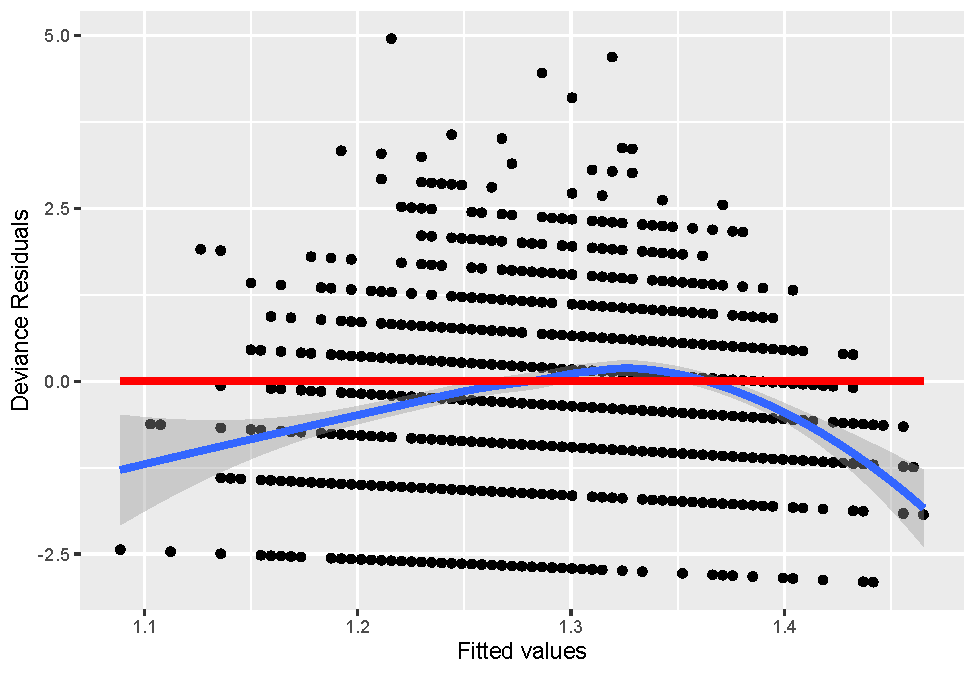
\includegraphics[width=0.6\linewidth]{bookdown-bysh_files/figure-latex/resid1-1} 

}

\caption{Residual plot for the Poisson model of household size by age of the household head}\label{fig:resid1}
\end{figure}

A plot (Figure \ref{fig:resid1}) of the deviance residuals versus predicted responses for the first order model exhibits curvature, supporting the idea that the model may improved by adding a quadratic term. Other details related to residual plots can be found in a variety of sources including \citet{McCullagh1989}.

\hypertarget{sec-PoisGOF}{%
\subsection{Goodness-of-fit}\label{sec-PoisGOF}}

The model residual deviance can be used to assess the degree to which the predicted values differ from the observed. When a model is true, we can expect the residual deviance to be distributed as a \(\chi^2\) random variable with degrees of freedom equal to the model's residual degrees of freedom. Our model thus far, the quadratic terms for age plus the indicators for location, has a residual deviance of 2187.8 with 1493 df. The probability of observing a deviance this large if the model fits is esentially 0, saying that there is significant evidence of lack-of-fit.

\begin{Shaded}
\begin{Highlighting}[]
\DecValTok{1}\OperatorTok{-}\KeywordTok{pchisq}\NormalTok{(modela2}\OperatorTok{$}\NormalTok{deviance, modela2}\OperatorTok{$}\NormalTok{df.residual)  }\CommentTok{# GOF test}
\end{Highlighting}
\end{Shaded}

\begin{verbatim}
[1] 0
\end{verbatim}

There are several reasons why \textbf{lack-of-fit} \index{lack of fit} may be observed. (1) We may be missing important covariates or interactions; a more comprehensive data set may be needed. (2) There may be extreme observations that may cause the deviance to be larger than expected; however, our residual plots did not reveal any unusual points. (3) Lastly, there may be a problem with the Poisson model. In particular, the Poisson model has only a single parameter, \(\lambda\), for each combination of the levels of the predictors which must describe both the mean and the variance. This limitation can become manifest when the variance appears to be larger than the corresponding means. In that case, the response is more variable than the Poisson model would imply, and the response is considered to be \textbf{overdispersed} \index{overdispersion}.

\hypertarget{linear-least-squares-regression-vs.-poisson-regression}{%
\section{\texorpdfstring{Linear Least Squares Regression \index{linear least squares regression (LLSR)} vs.~Poisson Regression \index{Poisson regression}}{Linear Least Squares Regression  vs.~Poisson Regression }}\label{linear-least-squares-regression-vs.-poisson-regression}}

\begin{gather*}
\underline{\textrm{Response}} \\
\mathbf{LLSR:}\textrm{ Normal} \\
\mathbf{Poisson Regression:}\textrm{ counts} \\
\textrm{ } \\
\underline{\textrm{Variance}} \\
\mathbf{LLSR:}\textrm{ Equal for each level of X} \\
\mathbf{Poisson Regression:}\textrm{ Equal to the mean for each level of X} \\
\textrm{ } \\
\underline{\textrm{Model Fitting}} \\
\mathbf{LLSR:}\ \mu=\beta_0+\beta_1x \textrm{ using Least Squares}\\
\mathbf{Poisson Regression:}\ log(\lambda)=\beta_0+\beta_1x \textrm{ using Maximum Likelihood}\\
\textrm{ } \\
\underline{\textrm{EDA}} \\
\mathbf{LLSR:}\textrm{ plot X vs. Y; add line} \\
\mathbf{Poisson Regression:}\textrm{ find }log(\bar{y})\textrm{ for several subgroups; plot vs. X} \\
\textrm{ } \\
\underline{\textrm{Comparing Models}} \\
\mathbf{LLSR:}\textrm{ extra sum of squares F-tests; AIC/BIC} \\
\mathbf{Poisson Regression:}\textrm{ Drop in Deviance tests; AIC/BIC} \\
\textrm{ } \\
\underline{\textrm{Interpreting Coefficients}} \\
\mathbf{LLSR:}\ \beta_1=\textrm{ change in }\mu_y\textrm{ for unit change in X} \\
\mathbf{Poisson Regression:}\ e^{\beta_1}=\textrm{ percent change in }\lambda\textrm{ for unit change in X} 
\end{gather*}

\hypertarget{case-study-campus-crime}{%
\section{Case Study: Campus Crime}\label{case-study-campus-crime}}

Students want to feel safe and secure when attending a college or university. In response to legislation, the US Department of Education seeks to provide data and reassurances to students and parents alike. All postsecondary institutions that participate in federal student aid programs are required by the Jeanne Clery Disclosure of Campus Security Policy and Campus Crime Statistics Act and the Higher Education Opportunity Act to collect and report data on crime occurring on campus to the Department of Education. In turn, this data is publicly available on the website of the Office of Postsecondary Education. We are interested in looking at whether there are regional differences in violent crime on campus, controlling for differences in the type of school.

\hypertarget{data-organization}{%
\subsection{Data Organization}\label{data-organization}}

Each row of \texttt{c\_data.csv} contains crime information from a post secondary institution, either a college or university. The variables include:

\begin{itemize}
\tightlist
\item
  \texttt{Enrollment} = enrollment at the school
\item
  \texttt{type} = college (C) or university (U)
\item
  \texttt{nv} = the number of violent crimes for that institution for the given year
\item
  \texttt{nvrate} = number of violent crimes per 1000 students
\item
  \texttt{enroll1000} = enrollment at the school, in thousands
\item
  \texttt{region} = region of the country (C = Central, MW = Midwest, NE = Northeast, SE = Southeast, SW = Southwest, and W = West)
\end{itemize}

\begin{verbatim}
# A tibble: 10 x 6
   Enrollment type     nv nvrate enroll1000 region
        <dbl> <chr> <dbl>  <dbl>      <dbl> <chr> 
 1       5590 U        30 5.37         5.59 SE    
 2        540 C         0 0            0.54 SE    
 3      35747 U        23 0.643       35.7  W     
 4      28176 C         1 0.0355      28.2  W     
 5      10568 U         1 0.0946      10.6  SW    
 6       3127 U         0 0            3.13 SW    
 7      20675 U         7 0.339       20.7  W     
 8      12548 C         0 0           12.5  W     
 9      30063 U        19 0.632       30.1  C     
10       4429 C         4 0.903        4.43 C     
\end{verbatim}

\hypertarget{exploratory-data-analysis}{%
\subsection{Exploratory Data Analysis}\label{exploratory-data-analysis}}

\begin{figure}

{\centering 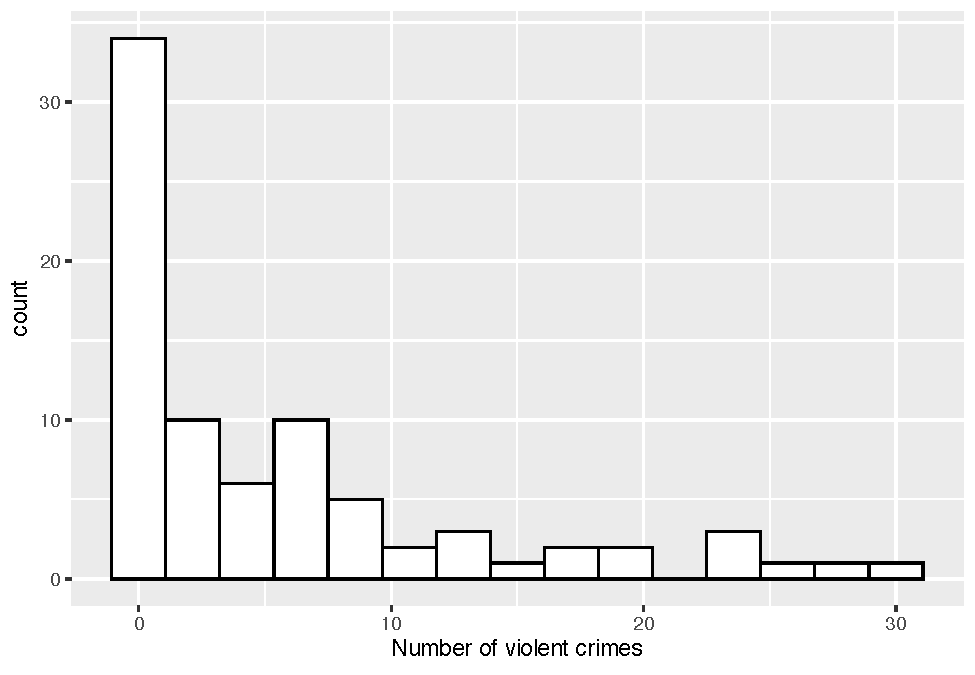
\includegraphics[width=0.6\linewidth]{bookdown-bysh_files/figure-latex/nviolent-1} 

}

\caption{Histogram of number of violent crimes by institution}\label{fig:nviolent}
\end{figure}

A graph of the number of violent crimes, Figure \ref{fig:nviolent}, reveals the pattern often found with distributions of counts of rare events. Many schools reported no violent crimes or very few crimes. A few schools have a large number of crimes making for a distribution that appears to be far from normal. Therefore, Poisson regression should be used to model our data; Poisson random variables are often used to represent counts (e.g., number of violent crimes) per unit of time or space (e.g., one year).

Let's take a look at two covariates of interest for these schools: type of institution and region. In our data, the majority of institutions are universities (65\% of the 81 schools) and only 35\% are colleges. Interest centers on whether the different regions tend to have different crime rates. Table \ref{tab:regions} contains the name of each region and each column represents the percentage of schools in that region which are colleges or universities. The proportion of colleges varies from a low of 20\% in the Southwest (SW) to a high of 50\% in the West (W).

\begin{table}

\caption{\label{tab:regions}Proportion of colleges and universities within region in the campus crime data set}
\centering
\begin{tabular}[t]{lrrrrrr}
\toprule
  & C & MW & NE & SE & SW & W\\
\midrule
C & 0.294 & 0.3 & 0.381 & 0.4 & 0.2 & 0.5\\
U & 0.706 & 0.7 & 0.619 & 0.6 & 0.8 & 0.5\\
\bottomrule
\end{tabular}
\end{table}

While a Poisson regression model is a good first choice because the responses are counts per year, it is important to note that the counts are not directly comparable because they come from different size schools. This issue sometimes is referred to as the need to account for \emph{sampling effort}; in other words, we expect schools with more students to have more reports of violent crime since there are more students who could be affected. We cannot directly compare the 30 violent crimes from the first school in the data set to no violent crimes for the second school when their enrollments are vastly different: 5,590 for school 1 versus 540 for school 2. We can take the differences in enrollments into account by including an \textbf{offset} in our model, which we will discuss in the next section. For the remainder of the EDA, we examine the violent crime counts in terms of the rate per 1,000 enrolled (\(\frac{\textrm{number of violent crimes}}{\textrm{number enrolled}} \cdot 1000\)).

Note that there is a noticeable outlier for a Southeastern school (5.4 violent crimes per 1000 students), and there is an observed rate of 0 for the Southwestern colleges which can lead to some computational issues. We therefore combined the SW and SE to form a single category of the South, and we also removed the extreme observation from the data set.

\begin{table}

\caption{\label{tab:table4ch4}The mean and variance of the violent crime rate by region and type of institution}
\centering
\begin{tabular}[t]{llrrrrr}
\toprule
region & type & MeanCount & VarCount & MeanRate & VarRate & n\\
\midrule
C & C & 1.6000 & 3.3000 & 0.3980 & 0.2781 & 5\\
C & U & 4.7500 & 30.9318 & 0.2219 & 0.0349 & 12\\
MW & C & 0.3333 & 0.3333 & 0.0163 & 0.0008 & 3\\
MW & U & 8.7143 & 30.9048 & 0.4019 & 0.0621 & 7\\
NE & C & 6.0000 & 32.8571 & 1.1250 & 1.1821 & 8\\
\addlinespace
NE & U & 5.9231 & 79.2436 & 0.4359 & 0.3850 & 13\\
S & C & 1.1250 & 5.8393 & 0.1866 & 0.1047 & 8\\
S & U & 8.6250 & 68.2500 & 0.5713 & 0.2778 & 16\\
W & C & 0.5000 & 0.3333 & 0.0680 & 0.0129 & 4\\
W & U & 12.5000 & 57.0000 & 0.4679 & 0.0247 & 4\\
\bottomrule
\end{tabular}
\end{table}

\begin{figure}

{\centering 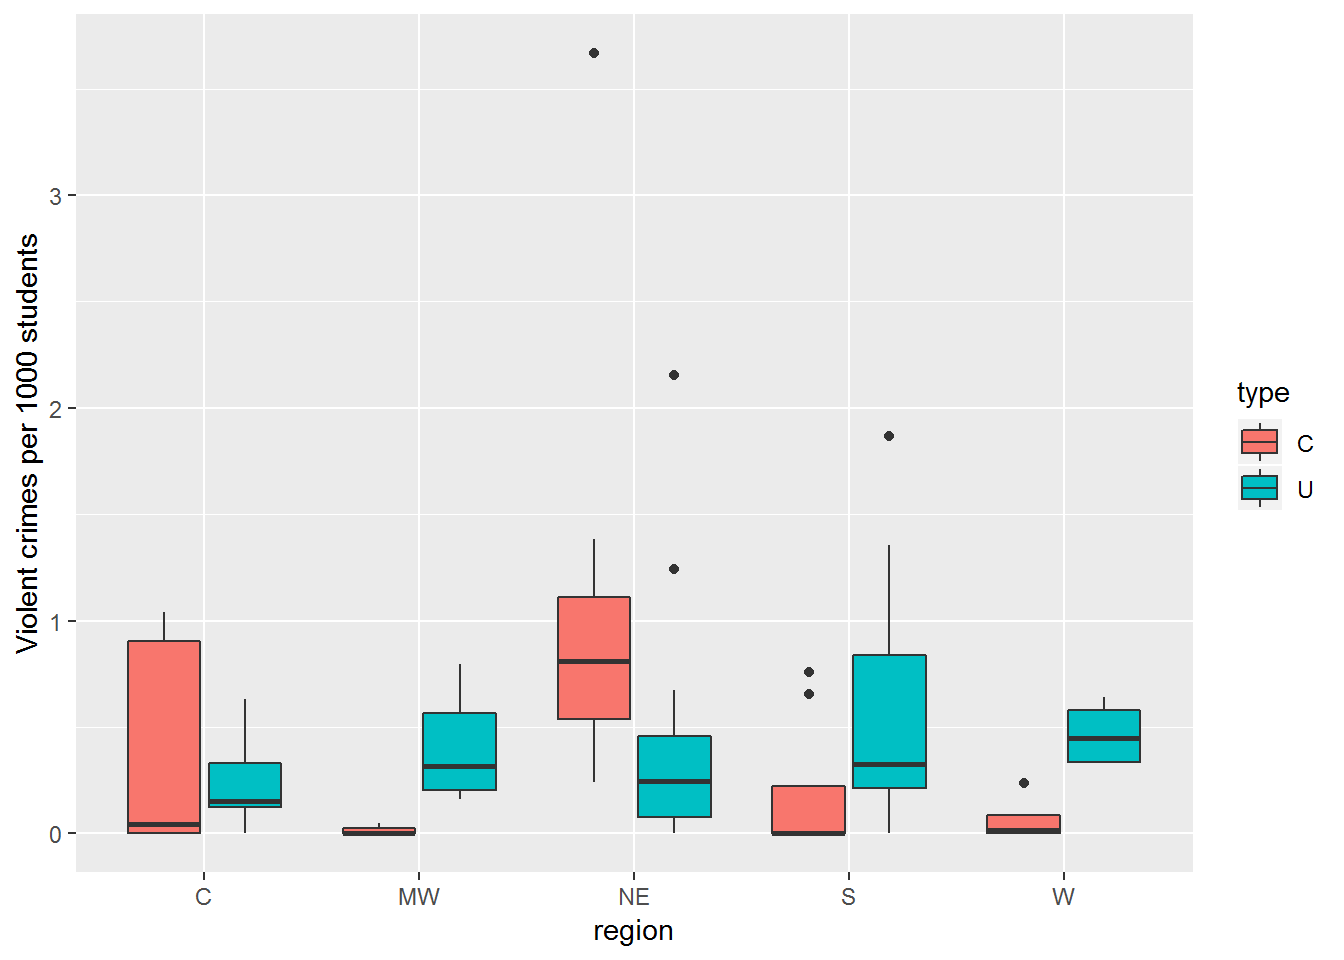
\includegraphics[width=0.6\linewidth]{bookdown-bysh_files/figure-latex/boxtyperegion-1} 

}

\caption{Boxplot of violent crime rate by region and type of institituion}\label{fig:boxtyperegion}
\end{figure}

Table \ref{tab:table4ch4} and Figure \ref{fig:boxtyperegion} display mean violent crime rates that are generally lower at the colleges within a region (with the exception of the Northeast). In addition, the regional pattern of rates at universities appears to differ from that of the colleges.

\hypertarget{accounting-for-enrollment}{%
\subsection{Accounting for Enrollment}\label{accounting-for-enrollment}}

Although working with the observed rates (per 1000 students) is useful during the exploratory data analysis, we do not use these rates explicitly in the model. The counts (per year) are the Poisson responses when modeling, so we must take into account the enrollment in a different way. Our approach is to include a term on the right side of the model called an \textbf{offset} \index{offset}, which is the log of the enrollment, in thousands. There is an intuitive heuristic for the form of the offset. If we think of \(\lambda\) as the mean number of violent crimes per year, then \(\lambda/\textrm{enroll1000}\) represents the number per 1000 students, so that the yearly count is adjusted to be comparable across schools of different sizes. Adjusting the yearly count by enrollment is equivalent to adding \(log(\textrm{enroll1000})\) to the right hand side of the Poisson regression equation---essentially adding a predictor with a fixed coefficient of 1:

\begin{align*} 
log(\frac{\lambda}{\textrm{enroll1000}} )= \beta_0 + \beta_1(\textrm{type}) \nonumber \\
log(\lambda)-log(\textrm{enroll1000}) = \beta_0 + \beta_1(\textrm{type}) \nonumber \\
log(\lambda) = \beta_0 + \beta_1(\textrm{type}) + log(\textrm{enroll1000})
\end{align*}

While this heuristic is helpful, it is important to note that it is \emph{not} \(\frac{\lambda}{ \textrm{enroll1000}}\) that we are modeling. We are still modeling \(log(\lambda)\), but we're adding an offset to adjust for differing enrollments, where the offset has the unusual feature that the coefficient is fixed at 1.0. As a result, no estimated coefficient for \texttt{enroll1000} or \(log(\textrm{enroll1000})\) will appear in the output. As this heuristic illustrates, modeling \(log(\lambda)\) and adding an offset is equivalent to modeling rates, and coefficients can be interpreted that way.

\hypertarget{modeling-assumptions}{%
\section{Modeling Assumptions}\label{modeling-assumptions}}

In Table \ref{tab:table4ch4}, we see that the variances are greatly higher than the mean counts in almost every group. Thus, we have reason to question the Poisson regression assumption of variability equal to the mean; we will have to return to this issue after some initial modeling. The fact that the variance of the rate of violent crimes per 1000 students tends to be on the same scale as the mean tells us that adjusting for enrollment may provide some help, although that may not completely solve our issues with excessive variance.

As far as other model assumptions, linearity with respect to \(log(\lambda)\) is difficult to discern without continuous predictors, and it is not possible to assess independence without knowing how the schools were selected.

\hypertarget{initial-models}{%
\section{Initial Models}\label{initial-models}}

We are interested primarily in differences in violent crime between institutional types controlling for difference in regions, so we fit a model with region, institutional type, and our offset. Note that the central region is the reference level in our model.

\begin{Shaded}
\begin{Highlighting}[]
\NormalTok{modeltr <-}\StringTok{ }\KeywordTok{glm}\NormalTok{(nv }\OperatorTok{~}\StringTok{ }\NormalTok{type }\OperatorTok{+}\StringTok{ }\NormalTok{region, }\DataTypeTok{family =}\NormalTok{ poisson,}
               \DataTypeTok{offset =} \KeywordTok{log}\NormalTok{(enroll1000), }\DataTypeTok{data =}\NormalTok{ c.data)}
\end{Highlighting}
\end{Shaded}

\begin{verbatim}
##             Estimate Std. Error z value  Pr(>|z|)
## (Intercept) -1.54780     0.1711 -9.0439 1.512e-19
## typeU        0.27956     0.1331  2.0997 3.576e-02
## regionMW     0.09912     0.1775  0.5583 5.766e-01
## regionNE     0.77813     0.1531  5.0836 3.703e-07
## regionS      0.58238     0.1490  3.9098 9.238e-05
## regionW      0.26275     0.1875  1.4011 1.612e-01
\end{verbatim}

\begin{verbatim}
##  Residual deviance =  348.7  on  74 df 
##  Dispersion parameter =  1
\end{verbatim}

From our model the Northeast and the South differ significantly from the Central region (p= 0.00000037 and p=0.0000924 respectively). The estimated coefficient of 0.778 means that the violent crime rate per 1,000 in the Northeast is nearly 2.2 (\(e^{0.778}\)) times that of the Central region controlling for the type of school. A Wald-type confidence interval for this factor can be constructed by first calculating a CI for the coefficient (0.778 \(\pm\) \(1.96 \cdot 0.153\)) and then exponentiating (1.61 to 2.94).

\hypertarget{tukeys-honestly-significant-differences}{%
\subsection{Tukey's Honestly Significant Differences}\label{tukeys-honestly-significant-differences}}

Comparisons to regions other than the Central region can be accomplished by changing the reference region. If many comparisons are made, it would be best to adjust for multiple comparisons using a method such as \textbf{Tukey's Honestly Significant Differences} \index{Tukey's honestly significant differences}, which considers all pairwise comparisons among regions. This method helps control the large number of false positives that we would see if we ran multiple t-tests comparing groups. The honestly significant difference compares a standardized mean difference between two groups to a critical value from a studentized range distribution.

\begin{Shaded}
\begin{Highlighting}[]
\NormalTok{mult_comp <-}\StringTok{ }\KeywordTok{summary}\NormalTok{(}\KeywordTok{glht}\NormalTok{(modeltr, }\KeywordTok{mcp}\NormalTok{(}\DataTypeTok{region=}\StringTok{"Tukey"}\NormalTok{)))}
\end{Highlighting}
\end{Shaded}

\begin{verbatim}
## # A tibble: 10 x 5
##    comparison estimate    SE z_value    p_value
##    <chr>         <dbl> <dbl>   <dbl>      <dbl>
##  1 MW - C       0.0991 0.178   0.558 0.980     
##  2 NE - C       0.778  0.153   5.08  0.00000349
##  3 S - C        0.582  0.149   3.91  0.000828  
##  4 W - C        0.263  0.188   1.40  0.621     
##  5 NE - MW      0.679  0.155   4.37  0.000109  
##  6 S - MW       0.483  0.151   3.19  0.0121    
##  7 W - MW       0.164  0.189   0.864 0.908     
##  8 S - NE      -0.196  0.122  -1.61  0.486     
##  9 W - NE      -0.515  0.166  -3.11  0.0157    
## 10 W - S       -0.320  0.163  -1.96  0.280
\end{verbatim}

In our case, Tukey's Honestly Significant Differences simultaneously evaluates all 10 mean differences between pairs of regions. We find that the Northeast has significantly higher rates of violent crimes than the Central, Midwest, and Western regions, while the South has significantly higher rates of violent crimes than the Central and the Midwest, controlling for the type of institution. In the primary model, the University indicator is significant and, after exponentiating the coefficient, can be interpreted as an approximately (\(e^{0.280}\)) 32\% increase in violent crime rate over colleges after controlling for region.

These results certainly suggest significant differences in regions and type of institution. However, the EDA findings suggest the effect of the type of institution may vary depending upon the region, so we consider a model with an interaction between region and type.

\begin{Shaded}
\begin{Highlighting}[]
\NormalTok{modeli <-}\StringTok{ }\KeywordTok{glm}\NormalTok{(nv }\OperatorTok{~}\StringTok{ }\NormalTok{type }\OperatorTok{+}\StringTok{ }\NormalTok{region }\OperatorTok{+}\StringTok{ }\NormalTok{region}\OperatorTok{:}\NormalTok{type, }
              \DataTypeTok{family =}\NormalTok{ poisson,}
              \DataTypeTok{offset =} \KeywordTok{log}\NormalTok{(enroll1000), }\DataTypeTok{data =}\NormalTok{ c.data)}
\end{Highlighting}
\end{Shaded}

\begin{verbatim}
##                Estimate Std. Error z value  Pr(>|z|)
## (Intercept)     -1.4741     0.3536 -4.1694 3.054e-05
## typeU            0.1959     0.3775  0.5190 6.038e-01
## regionMW        -1.9765     1.0607 -1.8635 6.239e-02
## regionNE         1.5529     0.3819  4.0664 4.775e-05
## regionS         -0.1562     0.4859 -0.3216 7.478e-01
## regionW         -1.8337     0.7906 -2.3194 2.037e-02
## typeU:regionMW   2.1965     1.0765  2.0403 4.132e-02
## typeU:regionNE  -1.0698     0.4200 -2.5473 1.086e-02
## typeU:regionS    0.8121     0.5108  1.5899 1.118e-01
## typeU:regionW    2.4106     0.8140  2.9616 3.061e-03
\end{verbatim}

\begin{verbatim}
##  Residual deviance =  276.7  on  70 df 
##  Dispersion parameter =  1
\end{verbatim}

These results provide convincing evidence of an interaction between the effect of region and the type of institution. A drop-in-deviance test like the one we carried out in the previous case study confirms the significance of the contribution of the interaction to this model. We have statistically significant evidence (\(\chi^2=71.98, df=4, p<.001\)) that the difference between colleges and universities in violent crime rate differs by region. For example, our model estimates that violent crime rates are 13.6 (\(e^{.196+2.411}\)) times higher in universities in the West compared to colleges, while in the Northeast we estimate that violent crime rates are 2.4 (\(\frac{1}{e^{.196-1.070}}\)) times higher in colleges.

\begin{Shaded}
\begin{Highlighting}[]
\NormalTok{drop_in_dev <-}\StringTok{ }\KeywordTok{anova}\NormalTok{(modeltr, modeli, }\DataTypeTok{test =} \StringTok{"Chisq"}\NormalTok{)}
\end{Highlighting}
\end{Shaded}

\begin{verbatim}
  ResidDF ResidDev Deviance Df      pval
1      74    348.7       NA NA        NA
2      70    276.7    71.98  4 8.664e-15
\end{verbatim}

The residual deviance (276.70 with 70 df) suggests significant lack of fit in the interaction model (p \textless{} .001). One possibility is that there are other important covariates that could be used to describe the differences in the violent crime rates. Without additional covariates to consider, we look for extreme observations, but we have already eliminated the most extreme of the observations.

In the absence of other covariates or extreme observations, we consider overdispersion as a possible explanation of the significant lack-of-fit.

\hypertarget{sec-overdispPois}{%
\section{Overdispersion}\label{sec-overdispPois}}

\hypertarget{dispersion-parameter-adjustment}{%
\subsection{Dispersion parameter adjustment}\label{dispersion-parameter-adjustment}}

\textbf{Overdispersion} \index{overdispersion} suggests that there is more variation in the response than the model implies. Under a Poisson model, we would expect the means and variances of the response to be about the same in various groups. Without adjusting for overdispersion, we use incorrect, artificially small standard errors leading to artificially small p-values for model coefficients. We may also end up with artificially complex models.

We can take overdispersion into account in several different ways. The simplest is to use an estimated dispersion factor to inflate standard errors. Another way is to use a negative-binomial regression model. We begin with using an estimate of the dispersion parameter.

We can estimate a dispersion parameter, \(\phi\), by dividing the model deviance by its corresponding degrees of freedom; i.e., \(\hat\phi=\frac{\sum(\textrm{Pearson residuals})^2}{n-p}\) where \(p\) is the number of model parameters. It follows from what we know about the \(\chi^2\) distribution that if there is no overdispersion, this estimate should be close to one. It will be larger than one in the presence of overdispersion. We inflate the standard errors by multiplying the variance by \(\phi\) so that the standard errors are larger than the likelihood approach would imply; i.e., \(SE_Q(\hat\beta)=\sqrt{\hat\phi}*SE(\hat\beta)\), where \(Q\) stands for ``quasi-Poisson'' \index{quasi-Poisson} since multiplying variances by \(\phi\) is an ad-hoc solution. Our process for model building and comparison is called \textbf{quasilikelihood} \index{quasilikelihood}---similar to likelihood but without exact underlying distributions. If we choose to use a dispersion parameter with our model, we refer to the approach as quasilikelihood. The following output illustrates a quasi-Poisson approach to the interaction model:

\begin{Shaded}
\begin{Highlighting}[]
\NormalTok{modeliq <-}\StringTok{ }\KeywordTok{glm}\NormalTok{(nv }\OperatorTok{~}\StringTok{ }\NormalTok{type }\OperatorTok{+}\StringTok{ }\NormalTok{region }\OperatorTok{+}\StringTok{ }\NormalTok{region}\OperatorTok{:}\NormalTok{type, }
               \DataTypeTok{family =}\NormalTok{ quasipoisson,}
               \DataTypeTok{offset =} \KeywordTok{log}\NormalTok{(enroll1000), }\DataTypeTok{data =}\NormalTok{ c.data)}
\end{Highlighting}
\end{Shaded}

\begin{verbatim}
##                Estimate Std. Error t value Pr(>|t|)
## (Intercept)     -1.4741     0.7455 -1.9773  0.05195
## typeU            0.1959     0.7961  0.2461  0.80631
## regionMW        -1.9765     2.2366 -0.8837  0.37987
## regionNE         1.5529     0.8053  1.9284  0.05786
## regionS         -0.1562     1.0246 -0.1525  0.87924
## regionW         -1.8337     1.6671 -1.0999  0.27513
## typeU:regionMW   2.1965     2.2701  0.9676  0.33659
## typeU:regionNE  -1.0698     0.8856 -1.2080  0.23111
## typeU:regionS    0.8121     1.0771  0.7540  0.45338
## typeU:regionW    2.4106     1.7164  1.4045  0.16460
\end{verbatim}

\begin{verbatim}
##  Residual deviance =  276.7  on  70 df 
##  Dispersion parameter =  4.447
\end{verbatim}

In the absence of overdispersion, we expect the dispersion parameter estimate to be 1.0. The estimated dispersion parameter here is much larger than 1.0 (4.447) indicating overdispersion (extra variance) that should be accounted for. The larger estimated standard errors in the quasi-Poisson model reflect the adjustment. For example, the standard error for the West region term from a likelihood based approach is 0.7906, whereas the quasilikelihood standard error is \(\sqrt{4.47}*0.7906\) or 1.6671. This term is no longer significant under the quasi-Poisson model. In fact, after adjusting for overdispersion (extra variation), none of the model coefficients in the quasi-Poisson model are significant at the .05 level! This is because standard errors were all increased by a factor of 2.1 (\(\sqrt{\hat\phi}=\sqrt{4.447}=2.1\)), while estimated coefficients remain unchanged.

Note that tests for individual parameters are now based on the t-distribution rather than a standard normal distribution, with test statistic \(t=\frac{\hat\beta}{SE_Q(\hat\beta)}\) following an (approximate) t-distribution with \(n-p\) degrees of freedom if the null hypothesis is true (\(H_O:\beta=0\)). Drop-in-deviance tests can be similarly adjusted for overdispersion in the quasi-Poisson model. In this case, you can divide the test statistic (per degree of freedom) by the estimated dispersion parameter and compare the result to an F-distribution with the difference in the model degrees of freedom for the numerator and the degrees of freedom for the larger model in the denominator. That is, \(F=\frac{\textrm{drop in deviance}}{\textrm{difference in df}} / {\hat\phi}\) follows an (approximate) F-distribution when the null hypothesis is true (\(H_0\): reduced model sufficient). The output below tests for an interaction between region and type of institution after adjusting for overdispersion (extra variance):

\begin{Shaded}
\begin{Highlighting}[]
\NormalTok{modeltrq <-}\StringTok{ }\KeywordTok{glm}\NormalTok{(nv }\OperatorTok{~}\StringTok{ }\NormalTok{type }\OperatorTok{+}\StringTok{ }\NormalTok{region, }\DataTypeTok{family =}\NormalTok{ quasipoisson,}
               \DataTypeTok{offset =} \KeywordTok{log}\NormalTok{(enroll1000), }\DataTypeTok{data =}\NormalTok{ c.data)}
\NormalTok{drop_in_dev <-}\StringTok{ }\KeywordTok{anova}\NormalTok{(modeltrq, modeliq, }\DataTypeTok{test =} \StringTok{"F"}\NormalTok{)}
\end{Highlighting}
\end{Shaded}

\begin{verbatim}
  ResidDF ResidDev     F Df     pval
1      74    348.7    NA NA       NA
2      70    276.7 4.047  4 0.005213
\end{verbatim}

Here, even after adjusting for overdispersion, we still have statistically significant evidence (\(F=4.05, p=.0052\)) that the difference between colleges and universities in violent crime rate differs by region.

\hypertarget{no-dispersion-vs.-overdispersion}{%
\subsection{No dispersion vs.~overdispersion}\label{no-dispersion-vs.-overdispersion}}

Table \ref{tab:compTable} summarizes the comparison between Poisson inference (tests and confidence intervals assuming no overdispersion) and quasi-Poisson inference (tests and confidence intervals after accounting for overdispersion).

\begin{table}

\caption{\label{tab:compTable}Comparison of Poisson and quasi-Poisson inference}
\centering
\resizebox{\linewidth}{!}{
\begin{tabular}[t]{lll}
\toprule
  & Poisson & quasi-Poisson\\
\midrule
Estimate & $\hat{\beta}$ & $\hat{\beta}$\\
Std error & $SE(\hat{\beta})$ & $SE_Q(\hat{\beta}) = \sqrt{\hat{\phi}} SE(\hat{\beta})$\\
Wald-type test stat & $Z = \hat{\beta} / SE(\hat{\beta})$ & $t = \hat{\beta} / SE_Q(\hat{\beta})$\\
Confidence interval & $\hat{\beta} \pm z^{'} SE(\hat{\beta})$ & $\hat{\beta} \pm t^{'} SE_Q(\hat{\beta})$\\
Drop in deviance test & $\chi^2 = \textrm{resid dev(reduced) - resid dev(full)}$ & $F = (\chi^2 / \textrm{difference in df}) / \hat{\phi}$\\
\bottomrule
\end{tabular}}
\end{table}

\hypertarget{negative-binomial-modeling}{%
\subsection{Negative binomial modeling}\label{negative-binomial-modeling}}

Another approach to dealing with overdispersion is to model the response using a negative binomial instead of a Poisson distribution. An advantage of this approach is that it introduces another parameter in addition to \(\lambda\) which gives the model more flexibility and, as opposed to the quasi-Poisson model, the negative binomial model assumes an explicit likelihood model. You may recall that negative binomial random variables take on nonnegative integer values which is consistent with modeling counts. This model posits selecting a \(\lambda\) for each institution and then generating a count using a Poisson random variable with the selected \(\lambda\). With this approach, the counts will be more dispersed than would be expected for observations based on a single Poisson variable with rate \(\lambda\). (See Guided Exercises on the Gamma-Poisson mixture in Chapter \ref{ch-distthry}.)

Mathematically, you can think of the negative binomial model as a Poisson model where \(\lambda\) is also random, following a gamma distribution. Specifically, if \(Y|\lambda \sim \textrm{Poisson}(\lambda)\) and \(\lambda \sim \textrm{gamma}(r,\frac{1-p}{p})\), then \(Y \sim \textrm{NegBinom}(r,p)\) where \(E(Y)=\frac{pr}{1-p}=\mu\) and \(Var(Y)=\frac{pr}{(1-p)^2}=\mu+\frac{\mu^2}{r}\). The overdispersion in this case is given by \(\frac{\mu^2}{r}\), which approaches 0 as \(r\) increases (so smaller values of \(r\) indicate greater overdispersion).

Here is what happens if we apply a negative binomial regression model \index{negative binomial regression} to the interaction model, which we've already established suffers from overdispersion issues under regular Poisson regression:

\begin{Shaded}
\begin{Highlighting}[]
\CommentTok{# Account for overdispersion with negative binomial model}
\NormalTok{modelinb <-}\StringTok{ }\KeywordTok{glm.nb}\NormalTok{(nv }\OperatorTok{~}\StringTok{ }\NormalTok{type }\OperatorTok{+}\StringTok{ }\NormalTok{region }\OperatorTok{+}\StringTok{ }\NormalTok{region}\OperatorTok{:}\NormalTok{type, }
               \KeywordTok{offset}\NormalTok{(}\KeywordTok{log}\NormalTok{(enroll1000)), }\DataTypeTok{data =}\NormalTok{ c.data2)}
\end{Highlighting}
\end{Shaded}

\begin{verbatim}
##                Estimate Std. Error z value Pr(>|z|)
## (Intercept)      0.4904     0.4281  1.1455 0.252008
## typeU            1.2174     0.4608  2.6422 0.008237
## regionMW        -1.0953     0.8075 -1.3563 0.175004
## regionNE         1.3966     0.5053  2.7641 0.005709
## regionS          0.1461     0.5559  0.2627 0.792752
## regionW         -1.1858     0.6870 -1.7260 0.084347
## typeU:regionMW   1.6342     0.8498  1.9231 0.054469
## typeU:regionNE  -1.1259     0.5601 -2.0102 0.044411
## typeU:regionS    0.4513     0.5995  0.7527 0.451638
## typeU:regionW    2.0387     0.7527  2.7086 0.006758
\end{verbatim}

\begin{verbatim}
##  Residual deviance =  199.6  on  69 df 
##  Dispersion parameter (theta) =  1.313
\end{verbatim}

These results differ from the quasi-Poisson model. Several effects are now statistically significant at the .05 level: the effect of type of institution for the Central region (\(Z=2.64, p=.008\)), the difference between Northeast and Central regions for colleges (\(Z=2.76, p=.006\)), the difference between Northeast and Central regions in type effect (\(Z=-2.01, p=.044\)), and the difference between West and Central regions in type effect (\(Z=2.71, p=.007\)). In this case, compared to the quasi-Poisson model, negative binomial coefficient estimates are generally in the same direction and similar in size, but negative binomial standard errors are somewhat smaller.

In summary, we explored the possibility of differences in the violent crime rate between colleges and universities, controlling for region. Our initial efforts seemed to suggest that there are indeed differences between colleges and universities, and the pattern of those differences depend upon the region. However, this model exhibited significant lack-of-fit which remained after the removal of an extreme observation. In the absence of additional covariates, we accounted for the lack-of-fit by using a quasilikelihood approach and a negative binomial regression, which provided slightly different conclusions. We may want to look for additional covariates and/or more data.

\hypertarget{cs:drinking}{%
\section{Case Study: Weekend drinking}\label{cs:drinking}}

Sometimes when analyzing Poisson data, you may see many more zeros in your data set than you would expect for a Poisson random variable. For example, an informal survey of students in an introductory statistics course included the question, ``How many alcoholic drinks did you consume last weekend?'' This survey was conducted on a dry campus where no alcohol is officially allowed, even among students of drinking age, so we expect that some portion of the respondents never drink. The non-drinkers would thus always report zero drinks. However, there will also be students who are drinkers reporting zero drinks because they just did not happen to drink during the past weekend. Our zeros, then, are a \textbf{mixture} of responses from non-drinkers and drinkers who abstained during the past weekend. Ideally, we'd like to sort out the non-drinkers and drinkers when performing our analysis.

\hypertarget{research-question}{%
\subsection{Research Question}\label{research-question}}

The purpose of this survey is to explore factors related to drinking behavior on a dry campus. What proportion of students on this dry campus never drink? What factors, such as off campus living and sex, are related to whether students drink? Among those who do drink, to what extent is moving off campus associated with the number of drinks in a weekend? It is commonly assumed that males' alcohol consumption is greater than females'; is this true on this campus? Answering these questions would be a simple matter if we knew who was and was not a drinker in our sample. Unfortunately, the non-drinkers did not identify themselves as such, so we will need to use the data available with a model that allows us to estimate the proportion of drinkers and non-drinkers.

\hypertarget{data-organization-1}{%
\subsection{Data Organization}\label{data-organization-1}}

Each line of \texttt{weekendDrinks.csv} contains data provided by a student in an introductory statistics course. In this analysis, the response of interest is the respondent's report of the number of alcoholic \texttt{drinks} they consumed the previous weekend, whether the student lives \texttt{off.campus}, and \texttt{sex}. We will also consider whether a student is likely a \texttt{firstYear} student based on the \texttt{dorm} they live in. Here is a sample of observations from this dataset:

\begin{Shaded}
\begin{Highlighting}[]
\KeywordTok{head}\NormalTok{(zip.data[}\DecValTok{2}\OperatorTok{:}\DecValTok{5}\NormalTok{])}
\end{Highlighting}
\end{Shaded}

\begin{verbatim}
  drinks sex off.campus firstYear
1      0   f          0      TRUE
2      5   f          0     FALSE
3     10   m          0     FALSE
4      0   f          0     FALSE
5      0   m          0     FALSE
6      3   f          0     FALSE
\end{verbatim}

\hypertarget{exploratory-data-analysis-1}{%
\subsection{Exploratory Data Analysis}\label{exploratory-data-analysis-1}}

As always we take stock of the amount of data; here there are 77 observations. Large sample sizes are preferred for the type of model we will consider, and n=77 is on the small side. We proceed with that in mind.

A premise of this analysis is that we believe that those responding zero drinks are coming from a mixture of non-drinkers and drinkers who abstained the weekend of the survey.

\begin{itemize}
\tightlist
\item
  \textbf{Non-drinkers}: respondents who never drink and would always reply with zero
\item
  \textbf{Drinkers}: obviously this includes those responding with one or more drinks, but it also includes people who are drinkers but did not happen to imbibe the past weekend. These people reply zero but are not considered non-drinkers.
\end{itemize}

\begin{figure}

{\centering 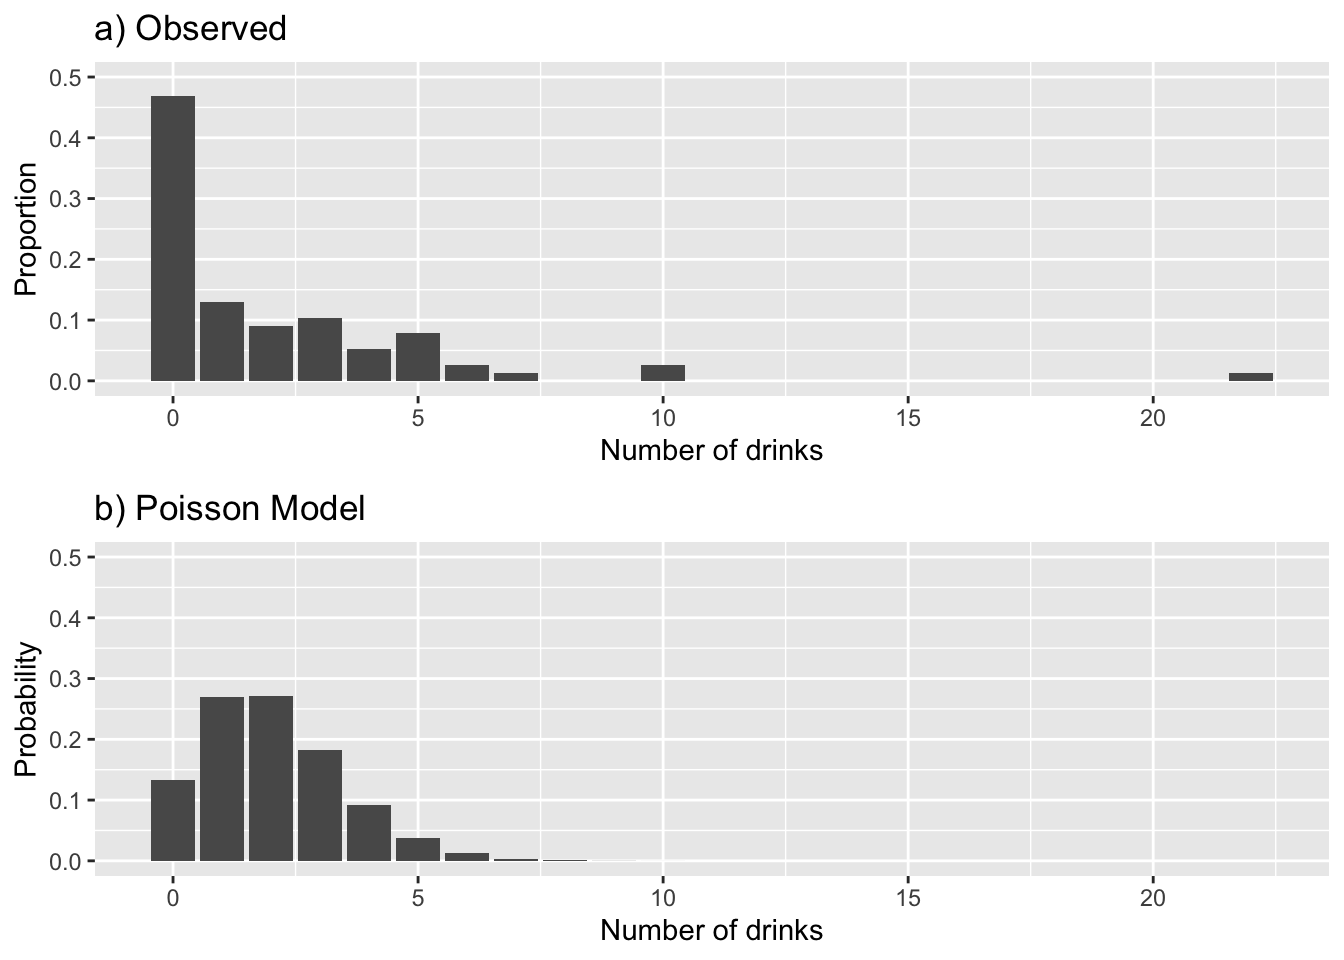
\includegraphics[width=0.6\linewidth]{bookdown-bysh_files/figure-latex/obsVmodel-1} 

}

\caption{Observed (a) versus Modeled (b) Number of Drinks}\label{fig:obsVmodel}
\end{figure}

Beginning the EDA with the response, number of drinks, we find that over 46\% of the students reported no drinks during the past weekend. Figure \ref{fig:obsVmodel}a portrays the observed number of drinks reported by the students. The mean number of drinks reported the past weekend is 2.013. Our sample consists of 74\% females and 26\% males, only 9\% of whom live off campus.

Because our response is a count, it is natural to consider a Poisson regression model. You may recall that a Poisson distribution has only one parameter, \(\lambda\), for its mean and variance. Here we will include an additional parameter, \(\alpha\). We define \(\alpha\) to be the true proportion of \emph{non-drinkers} in the population.

The next step in the EDA is especially helpful if you suspect your data contains excess zeros. Figure \ref{fig:obsVmodel}b is what we might expect to see under a Poisson model. Bars represent the probabilities for a Poisson distribution (using the Poisson probability formula) with \(\lambda\) equal to the mean observed number of drinks, 2.013 drinks per weekend. Comparing this Poisson distribution to what we observed (Figure \ref{fig:obsVmodel}a), it is clear that many more zeros have been reported by the students than you would expect to see if the survey observations were coming from a Poisson distribution. This doesn't surprise us because we had expected a subset of the survey respondents to be non-drinkers; i.e., they would not be included in this Poisson process. This circumstance actually arises in many Poisson regression settings. We will define \(\lambda\) to be the mean number of drinks \emph{among those who drink}, and \(\alpha\) to be the proportion of \emph{non-drinkers} (``true zeros''). Then, we will attempt to model \(\lambda\) and \(\alpha\) (or functions of \(\lambda\) and \(\alpha\)) simultaneously using covariates like sex, first-year status, and off-campus residence. This type of model is referred to as a \textbf{zero-inflated Poisson model} or \textbf{ZIP model} \index{zero-inflated Poisson}.

\hypertarget{modeling}{%
\subsection{Modeling}\label{modeling}}

We first fit a simple Poisson model with the covariates \texttt{off.campus} and \texttt{sex}.

\begin{Shaded}
\begin{Highlighting}[]
\NormalTok{pois.m1 <-}\StringTok{ }\KeywordTok{glm}\NormalTok{(drinks }\OperatorTok{~}\StringTok{ }\NormalTok{off.campus }\OperatorTok{+}\StringTok{ }\NormalTok{sex, }\DataTypeTok{family =}\NormalTok{ poisson,}
               \DataTypeTok{data =}\NormalTok{ zip.data)}
\end{Highlighting}
\end{Shaded}

\begin{verbatim}
##             Estimate Std. Error z value  Pr(>|z|)
## (Intercept)   0.1293     0.1241   1.041 2.976e-01
## off.campus    0.8976     0.2008   4.470 7.830e-06
## sexm          1.1154     0.1611   6.925 4.361e-12
\end{verbatim}

\begin{verbatim}
##  Residual deviance =  230.5  on  74 df 
##  Dispersion parameter =  1
\end{verbatim}

\begin{Shaded}
\begin{Highlighting}[]
\CommentTok{# Exponentiated coefficients}
\KeywordTok{exp}\NormalTok{(}\KeywordTok{coef}\NormalTok{(pois.m1))}
\end{Highlighting}
\end{Shaded}

\begin{verbatim}
## (Intercept)  off.campus        sexm 
##       1.138       2.454       3.051
\end{verbatim}

\begin{Shaded}
\begin{Highlighting}[]
\CommentTok{# Goodness-of-fit test}
\NormalTok{gof.pvalue =}\StringTok{ }\DecValTok{1} \OperatorTok{-}\StringTok{ }\KeywordTok{pchisq}\NormalTok{(pois.m1}\OperatorTok{$}\NormalTok{deviance, pois.m1}\OperatorTok{$}\NormalTok{df.residual)}
\NormalTok{gof.pvalue}
\end{Highlighting}
\end{Shaded}

\begin{verbatim}
## [1] 0
\end{verbatim}

Both covariates are statistically significant, but a goodness-of-fit test reveals that there remains significant lack-of-fit (residual deviance: 230.54 with only 74 df; p\textless.001 based on \(\chi^2\) test with 74 df). In the absence of important missing covariates or extreme observations, this lack-of-fit may be explained by the presence of a group of non-drinkers.

A zero-inflated Poisson regression model to take non-drinkers into account consists of two parts:

\begin{itemize}
\tightlist
\item
  One part models the association, among drinkers, between number of drinks and the predictors of sex and off campus residence.
\item
  The other part uses a predictor for first-year status to obtain an estimate of the proportion of non-drinkers based on the reported zeros.
\end{itemize}

The form for each part of the model follows. The first part looks like an ordinary Poisson regression model:

\[
log(\lambda)=\beta_0+\beta_1\textrm{off.campus}+ \beta_2\textrm{sex}
\]
where \(\lambda\) is the mean number of drinks in a weekend \emph{among those who drink}.
The second part has the form

\[
logit(\alpha)=\beta_0+\beta_1\textrm{firstYear}
\]
where \(\alpha\) is the probability of being in the non-drinkers group and \(logit(\alpha) = log( \alpha/(1-\alpha))\). We'll provide more detail on the logit in the Chapter \ref{ch-logreg}. There are many ways in which to structure this model; here we use different predictors in the two pieces, athough it would have been perfectly fine to use the same predictors for both pieces, or even no predictors for one of the pieces.

\hypertarget{fitting-a-zip-model}{%
\subsection{Fitting a ZIP Model}\label{fitting-a-zip-model}}

How is it possible to fit such a model? We cannot observe whether a respondent is a drinker or not (which probably would've been good to ask). The ZIP model is a special case of a more general type of statistical model referred to as a \textbf{latent variable model}. More specifically, it is a type of a \textbf{mixture model} \index{mixture model} where observations for one or more groups occur together and the group membership is unknown. Zero-inflated models are a particularly common example of a mixture model, but the response does not need to follow a Poisson distribution. Likelihood methods are at the core of this methodology, but fitting is an iterative process where it is necessary to start out with some guesses (or starting values). In general, it is important to know that models like ZIP exist, although we'll only explore interpretations and fitting options for a single case study here.

Here is the general idea of how ZIP models are fit. Imagine that the graph of the Poisson distribution in Figure \ref{fig:obsVmodel}b is removed from the observed data distribution in Figure \ref{fig:obsVmodel}a. Some zero responses will remain. These would correspond to non-drinkers, and the proportion of all observations these zeros constitute might make a reasonable estimate for \(\alpha\), the proportion of non-drinkers. The likelihood is used and some iterating in the fitting process is involved because the Poisson distribution in Figure \ref{fig:obsVmodel}b is based on the mean of the observed data, which means it is the average among all students, not only among drinkers. Furthermore, the likelihood incorporates the predictors, \texttt{sex} and \texttt{off.campus}. So there is a little more to it than computing the proportion of zeros, but this heuristic should provide you a general idea of how these kinds of models are fit. We will use the R function \texttt{zeroinfl} from the package \texttt{pscl} to fit a ZIP model.

\begin{Shaded}
\begin{Highlighting}[]
\NormalTok{zip.m2 <-}\StringTok{ }\KeywordTok{zeroinfl}\NormalTok{(drinks }\OperatorTok{~}\StringTok{ }\NormalTok{off.campus }\OperatorTok{+}\StringTok{ }\NormalTok{sex }\OperatorTok{|}\StringTok{ }\NormalTok{firstYear, }
                   \DataTypeTok{data =}\NormalTok{ zip.data)}
\end{Highlighting}
\end{Shaded}

\begin{verbatim}
## $count
##             Estimate Std. Error z value  Pr(>|z|)
## (Intercept)   0.7543     0.1440   5.238 1.624e-07
## off.campus    0.4159     0.2059   2.020 4.333e-02
## sexm          1.0209     0.1752   5.827 5.634e-09
## 
## $zero
##               Estimate Std. Error z value Pr(>|z|)
## (Intercept)    -0.6036     0.3114  -1.938  0.05261
## firstYearTRUE   1.1364     0.6095   1.864  0.06226
\end{verbatim}

\begin{verbatim}
##  Log likelihood =  -140.8
\end{verbatim}

\begin{Shaded}
\begin{Highlighting}[]
\KeywordTok{exp}\NormalTok{(}\KeywordTok{coef}\NormalTok{(zip.m2))   }\CommentTok{# exponentiated coefficients}
\end{Highlighting}
\end{Shaded}

\begin{verbatim}
##  count_(Intercept)   count_off.campus 
##             2.1261             1.5158 
##         count_sexm   zero_(Intercept) 
##             2.7757             0.5468 
## zero_firstYearTRUE 
##             3.1155
\end{verbatim}

Our model uses \texttt{firstYear} to distinguish drinkers and non-drinkers (``Zero-inflation model coefficients'') and \texttt{off.campus} and \texttt{sex} to help explain the differences in the number of drinks among drinkers (``Count model coefficients''). Again, we could have used the same covariates for the two pieces of a ZIP model, but neither \texttt{off.campus} or \texttt{sex} proved to be a useful predictor of drinkers vs.~non-drinkers after we accounted for first-year status.

We'll first consider the ``Count model coefficients,'' which provide information on how the sex and off-campus status of a student who is a drinker are related to the number of drinks reported by that student over a weekend. As we have done with previous Poisson regression models, we exponentiate each coefficient for ease of interpretation. Thus, for those who drink, the average number of drinks for males is \(e^{1.0209}\) or 2.76 times the number for females (Z = 5.827, p \textless{} 0.001) given that you are comparing people who live in comparable settings, i.e., either both on or both off campus. Among drinkers, the mean number of drinks for students living off campus is \(e^{0.4159}=1.52\) times that of students living on campus for those of the same sex (Z = 2.021, p = 0.0433).

The ``Zero-inflation model coefficients'' refer to separating drinkers from non-drinkers. An important consideration in separating drinkers from non-drinkers may be whether this is their first year, where \texttt{firstYear} is a 0/1 indicator variable.

We have
\[ 
log(\alpha/(1-\alpha)) =-0.6036+1.1364\textrm{firstYear}
 \]

However we are interested in \(\alpha\), the proportion of non-drinkers. Exponentiating the coefficient for the first year term for this model yields 3.12. Here it is interpreted as the odds (\(\frac{\alpha}{1-\alpha}\)) that a first year is a non-drinker is 3.12 times the odds that an upper class student is a non-drinker. Furthermore, with a little algebra (solving the equation with \(log(\alpha/(1-\alpha)\)) for \(\alpha\)),
we have

\[
 \hat{\alpha} =
 \frac{e^ {-0.6036+1.1364(\textrm{firstYear})}}
 {1+e^{
 -0.6036+1.1364(\textrm{firstYear})
 }
 }.
 \]

The estimated chance that a first year student is a non-drinker is

\[
\frac{e^{0.533}}{1+e^{0.533}} = 0.630
\]
or 63.0\%, while for non-first years, the estimated probability of being a non-drinker is 0.354. If you have seen logistic regression, you'll recognize that this transformation is what is used to estimate a probability. More on this in the Logistic Regression chapter.

\hypertarget{comparing-zip-to-ordinary-poisson-with-the-vuong-test-optional}{%
\subsection{Comparing ZIP to ordinary Poisson with the Vuong Test (Optional)}\label{comparing-zip-to-ordinary-poisson-with-the-vuong-test-optional}}

Moving from ordinary Poisson to zero-inflated Poisson has helped us address additional research questions: What proportion of students are non-drinkers and what factors are associated with whether or not a student is a non-drinker? While a ZIP model seems more faithful to the nature and structure of this data, can we quantitatively show that a zero-inflated Poisson is better than an ordinary Poisson model?

We cannot use the drop-in-deviance test we discussed earlier because these two models are not nested within one another. Vuong \citeyearpar{Vuong1989} devised a test to make this comparison for the special case of comparing a zero-inflated model and ordinary regression model. Essentially, the Vuong Test \index{Vuong test} is able to compare predicted probabilities of \textbf{non-nested} models.

\begin{Shaded}
\begin{Highlighting}[]
\KeywordTok{vuong}\NormalTok{(pois.m1, zip.m2)}
\end{Highlighting}
\end{Shaded}

\begin{verbatim}
Vuong Non-Nested Hypothesis Test-Statistic: 
(test-statistic is asymptotically distributed N(0,1) under the
 null that the models are indistinguishible)
-------------------------------------------------------------
              Vuong z-statistic             H_A
Raw                      -2.689 model2 > model1
AIC-corrected            -2.534 model2 > model1
BIC-corrected            -2.353 model2 > model1
              p-value
Raw            0.0036
AIC-corrected  0.0056
BIC-corrected  0.0093
\end{verbatim}

Here, we have structured the Vuong Test to compare Model 1: Ordinary Poisson Model to Model 2: Zero-inflation Model. If the two models do not differ, the test statistic for Vuong would be asymptotically standard Normal and the p-value would be relatively large. Here the first line of the output table indicates that the zero-inflation model is better (\(Z=-2.69,p=.0036\)). Note that the test depends upon sufficiently large n for the Normal approximation, so since our sample size (n=77) is somewhat small, we need to interpret this result with caution. More research is underway to address statistical issues related to these comparisons.

\hypertarget{residual-plot}{%
\subsection{Residual Plot}\label{residual-plot}}

Fitted values (\(\hat{y}\)) and residuals (\(y-\hat{y}\)) can be computed for zero-inflation models and plotted. Figure \ref{fig:poisRes} reveals that one observation appears to be extreme (Y=22 drinks during the past weekend). Is this a legitimate observation or was there a transcribing error? Without the original respondents we cannot settle this question. It might be worthwhile to get a sense of how influential this extreme observation is by removing Y=22 and refitting the model.

\begin{figure}

{\centering 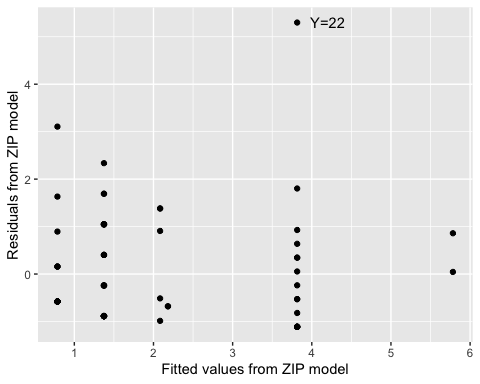
\includegraphics[width=0.6\linewidth]{bookdown-bysh_files/figure-latex/poisRes-1} 

}

\caption{Residuals by fitted counts for ZIP model.}\label{fig:poisRes}
\end{figure}

\hypertarget{limitations}{%
\subsection{Limitations}\label{limitations}}

Given that you have progressed this far in your statistical education, the weekend drinking survey question should raise some red flags. What time period constitutes the ``weekend''? Will some students be thinking of only Saturday night while others include Friday night or possibly Sunday evening? What constitutes a drink---a bottle of beer? How many drinks will a respondent report for a bottle of wine? Precise definitions would vastly improve the quality of this data. There is also an issue related to confidentiality. If the data is collected in class, will the teacher be able to identify the respondent? Will respondents worry that a particular response will affect their grade in the class or lead to repercussions on a dry campus?

In addition to these concerns, there are a number of other limitations that should be noted. Following the concern of whether this data represents a random sample of any population (it doesn't), we also must be concerned with the size of this data set. ZIP models are not appropriate for small samples and this data set is not impressively large.

At times, a mixture of zeros occurs naturally. It may not come about because of neglecting to ask a critical question on a survey, but the information about the subpopulation may simply not be ascertainable. For example, visitors from a state park were asked as they departed how many fish they caught, but those who report 0 could be either non-fishers or fishers who had bad luck. These kinds of circumstances occur often enough that ZIP models are becoming increasingly common.

Actually, applications which extend beyond ordinary Poisson regression applications---ZIPs and other Poisson modeling approaches such as hurdle models and quasi-Poisson applications---are becoming increasingly common. So it is worth taking a look at these variations of Poisson regression models. Here we have only skimmed the surface of zero-inflated models, but we want you to be aware of models of this type. ZIP models demonstrate that modeling can be flexible and creative---a theme we hope you will see throughout this book.

\hypertarget{exercises}{%
\section{Exercises}\label{exercises}}

\hypertarget{exer:concept}{%
\subsection{Conceptual Exercises}\label{exer:concept}}

Exercises 1-4 involve predicting a \textbf{response} using one or more \textbf{explanatory variables}, where these examples have response variables that are counts per some unit of time or space. List the response (both what is being counted and over what unit of time or space) and relevant explanatory variables.

\begin{enumerate}
\def\labelenumi{\arabic{enumi}.}
\tightlist
\item
  Are the number of motorcycle deaths in a given year related to a state's helmet laws?
\item
  Does the number of employers conducting on-campus interviews during a year differ for public and private colleges?
\item
  Does the daily number of asthma-related visits to an Emergency Room differ depending on air pollution indices?
\item
  Has the number of deformed fish in randomly selected Minnesota lakes been affected by changes in trace minerals in the water over the last decade?
  \vspace{3mm}
\item
  Models of the form \(Y_i=\beta_0+\beta_1X_i+\epsilon_i, \epsilon_i \sim iidN(0,\sigma)\) are fit using the method of least squares. What method is used to fit Poisson regression models?
\item
  What should be done before adjusting for overdispersion?
\item
  Why are quasi-Poisson models used, and how do the results typically compare for corresponding models using regular Poisson regression?
\item
  Why is the log of mean counts, log(\(\bar{Y}\)), not \(\bar{Y}\), plotted against X when assessing the assumptions for Poisson regression?
\item
  How can the assumption of \emph{mean=variance} be checked for Poisson regression? What if there are not many repeated observations at each level of X?
\item
  Is it possible that a predictor is significant for a model fit using Poisson regression, but not for a model for the same data fit using quasi-Poisson regression? Explain.
\end{enumerate}

Complete (a)-(d) in the context of the study for Exercises 11-13.

\begin{enumerate}
\def\labelenumi{\alph{enumi}.}
\tightlist
\item
  Define the response.
\item
  What are the possible values for the response?
\item
  What does \(\lambda\) represent?
\item
  Would a zero-inflated model be considered here? If so, what would be a ``true zero?''
\end{enumerate}

\begin{enumerate}
\def\labelenumi{\arabic{enumi}.}
\setcounter{enumi}{10}
\item
  \textbf{Fish (or, as they say in French, poisson)} A state wildlife biologist collected data from 250 park visitors as they left at the end of their stay. Each was asked to report the number of fish they caught during their one week stay. On average visitors caught 21.5 fish per week.
\item
  \textbf{Methadone Program Recidivism.} Program facilitators keep track of the number of times their program's patients relapse within five years of initial treatment. Data on 100 patients yielded a mean number of 2.8 relapses per patient within the five years of initial treatment.
\item
  \textbf{Clutch size.} Thirty nests were located and the number of eggs in each nest were counted at the start of a season. Later in the season following a particularly destructive storm, the mean clutch size of the 30 nests was only 1.7 eggs per nest.
  \vspace{3mm}
\item
  \textbf{Credit card use} A survey of 1,000 consumers asked respondents how many credit cards they use. Interest centers on the relationship between credit card use and income, in \$10,000. The estimated coefficient for income is 2.1.

  \begin{itemize}
  \tightlist
  \item
    Identify the predictor and interpret the estimated coefficient for the predictor in this context.
  \item
    Describe how the assumption of linearity can be assessed in this example.
  \item
    Suggest a way in which to assess the equal mean and variance assumption.
  \end{itemize}
\end{enumerate}

\begin{table}

\caption{\label{tab:tab2chp4}Sample data for Exercise 15}
\centering
\begin{tabular}[t]{rrr}
\toprule
Age & Time online & Number of dates arranged online\\
\midrule
19 & 35 & 3\\
29 & 20 & 5\\
38 & 15 & 0\\
55 & 10 & 0\\
\bottomrule
\end{tabular}
\end{table}

\begin{enumerate}
\def\labelenumi{\arabic{enumi}.}
\setcounter{enumi}{14}
\item
  \textbf{Dating Online} Researchers are interested in the number of dates respondents arranged online and whether the rates differ by age group. Questions which elicit responses similar to this can be found in the Pew survey concerning dating online and relationships \citep{Duggan2013}. Each survey respondent was asked how many dates they have arranged online in the past 3 months as well as the typical amount of time, \(t\), in hours, they spend online weekly. Some rows of data appear in Table \ref{tab:tab2chp4}.

  \begin{itemize}
  \tightlist
  \item
    Identify the response, predictor, and offset in this context. Does using an offset make sense?
  \item
    Write out a model for this data. As part of your model description, define the parameter, \(\lambda\).
  \item
    Consider a Zero-inflated Poisson model for this data. Describe what the `true zeros' would be in this setting.
  \end{itemize}
\end{enumerate}

\begin{table}

\caption{\label{tab:tab3chp4}Data from Scotto et al. (1974) on the number of cases of non melanoma skin cancer for women by age group in two metropolitan areas (Minneapolis-St Paul and Dallas-Ft Worth); the year is unknown. The columns contain: number of cases of skin cancer, population size of the age group per city, age group, and metropolitan area (1=Minneapolis-St Paul, 2=Dallas-Ft Worth).}
\centering
\begin{tabular}[t]{l|l|l|l}
\hline
Number of Cases & Population & Age Group & City\\
\hline
1 & 172675 & 15-24 & 1\\
\hline
16 & 123065 & 25-34 & 1\\
\hline
... & ... & ... & ...\\
\hline
226 & 29007 & 75-84 & 2\\
\hline
65 & 7538 & 85+ & 2\\
\hline
\end{tabular}
\end{table}

\begin{enumerate}
\def\labelenumi{\arabic{enumi}.}
\setcounter{enumi}{15}
\item
  \textbf{Poisson Approximation: Rare Events} For rare diseases, the probability of a case occurring, \(p\), in a very large population, \(n\), is small. With a small \(p\) and large \(n\), the random variable \(Y\)= the number of cases out of \(n\) people can be approximated using a Poisson random variable with \(\lambda = np\). If the count of those with the disease is observed in several different populations independently of one another, the \(Y_i\) represents the number of cases in the \(i^{th}\) population and can be approximated using a Poisson random variable with \(\lambda_i=n_ip_i\) where \(p_i\) is the probability of a case for the \(i^{th}\) population. Poisson regression can take into account the differences in the population sizes, \(n_i\), using as an offset log(\(n_i\)) as well as differences in a population characteristic like \(x_i\). The coefficient of the offset is set at one; it is not estimated like the other coefficients. Thus the model statement has the form: \(log(\lambda_i) = \beta_0+\beta_1x_i + log(n_i)\), where \(Y_i \sim\) Poisson(\(\lambda_i = n_i p_i\)). Note that \(\lambda_i\) depends on \(x_i\) which may differ for the different populations.

  \citet{Scotto1974} wondered if skin cancer rates by age group differ by city. Based on their data in Table \ref{tab:tab3chp4}, identify and describe the following quantities which appear in the description of the Poisson approximation for rare events:

  \begin{itemize}
  \tightlist
  \item
    A case,
  \item
    The population size, \(n_i\),
  \item
    Probability, \(p_i\),
  \item
    Poisson parameter, \(\lambda_i\),
  \item
    Poisson random variables, \(Y_i\), and
  \item
    The predictors, \(X_i\).
  \end{itemize}
\end{enumerate}

\hypertarget{guided-exercises}{%
\subsection{Guided Exercises}\label{guided-exercises}}

\begin{enumerate}
\def\labelenumi{\arabic{enumi}.}
\tightlist
\item
  \textbf{College Burglaries} We wish to build a regression model to describe the number of burglaries on a college campus in a year. Our population of interest will be U.S. liberal arts colleges.

  \begin{enumerate}
  \def\labelenumii{\alph{enumii}.}
  \tightlist
  \item
    Describe why the response variable (\(Y\) = \# burglaries on campus in a year) could be modeled by a Poisson distribution.
  \item
    Describe explanatory variables which might explain differences in \(\lambda_i\) = mean number of burglaries per year on campus \(i\).
  \item
    Consider a campus with an average of 5 burglaries per year. Use \texttt{dpois()} to sketch a plot of the distribution of \(Y\) for this campus. Use \texttt{rpois()} to verify that both the mean and variance of \(Y\) are given by \(\lambda=5\).
  \item
    Consider a campus with an average of 20 burglaries per year and repeat (c).
  \end{enumerate}
\item
  \textbf{Elephant Mating} How does age affect male elephant mating patterns? An article by \citet{Poole1989} investigated whether mating success in male elephants increases with age and whether there is a peak age for mating success. To address this question, the research team followed 41 elephants for one year and recorded both their ages and their number of matings. The data \citep{Ramsey2002} is found in \texttt{elephant.csv}, and the variables are:

  \begin{itemize}
  \tightlist
  \item
    \texttt{MATINGS} = the number of matings in a given year
  \item
    \texttt{AGE} = the age of the elephant in years.
  \end{itemize}

  \begin{enumerate}
  \def\labelenumii{\alph{enumii}.}
  \tightlist
  \item
    Create a histogram of MATINGS. Is there preliminary evidence that number of matings could be modeled as a Poisson response? Explain.
  \item
    Plot MATINGS by AGE. Add a least squares line. Is there evidence that modeling matings using a linear regression with age might not be appropriate? Explain. (Hints: fit a smoother; check residual plots)
  \item
    For each age, calculate the mean number of matings. Take the log of each mean and plot it by AGE.

    \begin{enumerate}
    \def\labelenumiii{\roman{enumiii}.}
    \tightlist
    \item
      What assumption can be assessed with this plot?
    \item
      Is there evidence of a quadratic trend on this plot?
    \end{enumerate}
  \item
    Fit a Poisson regression model with a linear term for AGE. Exponentiate and then interpret the coefficient for AGE.
  \item
    Construct a 95\% confidence interval for the slope and interpret in context (you may want to exponentiate endpoints).
  \item
    Are the number of matings significantly related to age? Test with

    \begin{enumerate}
    \def\labelenumiii{\roman{enumiii}.}
    \tightlist
    \item
      a Wald test and
    \item
      a drop in deviance test.
    \end{enumerate}
  \item
    Add a quadratic term in AGE to determine whether there is a maximum age for the number of matings for elephants. Is a quadratic model preferred to a linear model? To investigate this question, use

    \begin{enumerate}
    \def\labelenumiii{\roman{enumiii}.}
    \tightlist
    \item
      a Wald test and
    \item
      a drop in deviance test.
    \end{enumerate}
  \item
    What can we say about the goodness of fit of the model with age as the sole predictor? Compare the residual deviance for the linear model to a \(\chi^2\) distribution with the residual model degrees of freedom.
  \item
    Fit the linear model using quasi-Poisson regression. (Why?)

    \begin{enumerate}
    \def\labelenumiii{\roman{enumiii}.}
    \tightlist
    \item
      How do the estimated coefficients change?
    \item
      How do the standard errors change?
    \item
      What is the estimated dispersion parameter?
    \item
      An estimated dispersion parameter greater than one suggests overdispersion. When adjusting for overdispersion, are you more or less likely to obtain a significant result when testing coefficients? Why?
    \end{enumerate}
  \end{enumerate}
\end{enumerate}

\begin{table}

\caption{\label{tab:ex3chp4}A small subset of hypothetical data on Minnesota workplace rules on smoking.  X is 0 for home and 1 for work.  Y is number of cigaretttes in a 2-hour period.}
\centering
\begin{tabular}[t]{rrr}
\toprule
Subject & X (location) & Y (cigarettes)\\
\midrule
1 & 0 & 3\\
2 & 1 & 0\\
3 & 1 & 0\\
4 & 1 & 1\\
5 & 0 & 2\\
\addlinespace
6 & 0 & 1\\
\bottomrule
\end{tabular}
\end{table}

\begin{enumerate}
\def\labelenumi{\arabic{enumi}.}
\setcounter{enumi}{2}
\item
  \textbf{Smoking at Work and Home} An earlier study examined the effect of workplace rules in Minnesota which require smokers to smoke cigarettes outside. The number of cigarettes smoked by smokers in a 2-hour period was recorded, along with whether the smoker was at home or at work. A (very) small subset of the data appears in Table \ref{tab:ex3chp4}.

  \begin{itemize}
  \tightlist
  \item
    Model 1: Assume that \(Y \sim \textrm{Poisson}(\lambda)\); there is no difference between home and work.
  \item
    Model 2: Assume that \(Y \sim \textrm{Poisson}(\lambda_W)\) when the smoker is at work, and \(Y \sim \textrm{Poisson}(\lambda_H)\) when the smoker is at home.
  \item
    Model 3: Assume that \(Y \sim \textrm{Poisson}(\lambda)\) and \(log(\lambda)=\beta_0+\beta_1X\).
  \end{itemize}

  \begin{enumerate}
  \def\labelenumii{\alph{enumii}.}
  \tightlist
  \item
    Write out the likelihood \(L(\lambda)\) and the log-likelihood \(logL(\lambda)\) in Model 1. Use the data values above, and simplify where possible.
  \item
    Intuitively, what would be a reasonable estimate for \(\lambda\) based on this data? Why?
  \item
    Find the maximum likelihood estimator for \(\lambda\) in Model 1 using an optimization routine in R (but not the \texttt{glm()} function). Use R to produce a plot of the likelihood function \(L(\lambda)\).
  \item
    Write out the log-likelihood function \(logL(\lambda_W, \lambda_H)\) in Model 2. Use the data values above, and simplify where possible.
  \item
    Intuitively, what would be reasonable estimates for \(\lambda_W\) and \(\lambda_H\) based on this data? Why?
  \item
    Find the maximum likelihood estimators for \(\lambda_W\) and \(\lambda_H\) in Model 2 using an optimization routine in R (but not the \texttt{glm()} function).
  \end{enumerate}
\item
  \textbf{Smoking at Work and Home (continued)} We will use the same dataset in this question as we used in question 3.

  \begin{enumerate}
  \def\labelenumii{\alph{enumii}.}
  \tightlist
  \item
    Write out the log-likelihood function \(logL(\beta_0, \beta_1)\) in Model 3. Again, use the data values above, and simplify where possible.
  \item
    Find the maximum likelihood estimators for \(\beta_0\) and \(\beta_1\) in Model 3 using an optimization routine in R (but not the \texttt{glm()} function). Use R to produce a 3D plot of the log-likelihood function.
  \item
    Confirm your estimates for Model 1 and Model 3 using \texttt{glm()}. Then show that the MLEs for Model 3 agree with the MLEs for Model 2.
  \end{enumerate}

  For the remaining questions, we will focus exclusively on Model 3.

  \begin{enumerate}
  \def\labelenumii{\alph{enumii}.}
  \setcounter{enumii}{3}
  \tightlist
  \item
    State a (one-sided) hypothesis for \(\beta_1\) in the context of the problem (i.e.~explain how your hypothesis relates to smoking at home and at work). Note: we will nevertheless use two-sided tests and intervals in the following questions.
  \item
    Do we need to include an offset in our Poisson regression model? Why or why not?
  \item
    Give estimates of \(\beta_0\) and \(\beta_1\), and provide interpretations for both in the context of the problem.
  \item
    Provide and interpret a 95\% confidence interval for \(\beta_1\).
  \item
    Provide two \emph{different} significance tests for \(\beta_1\), in each case providing a test statistic and a p-value and a conclusion in the context of the problem.
  \item
    Provide a goodness-of-fit test for Model 3, again providing a test statistic, p-value, and conclusion in context.
  \item
    Can we generalize results of this study to all Minnesota smokers? Why or why not?
  \item
    Can we claim that rules restricting smoking in the workplace have caused lower levels of smoking at work? Explain.
  \item
    Give two ways in which this study might be improved (besides simply ``bigger sample size'').
  \end{enumerate}
\item
  \textbf{Campus Crime} The data set \texttt{campuscrime09.csv} contains the number of burglaries reported at a collection of 47 US public universities with over 10,000 students in the year 2009. In addition, covariates are included which may explain differences in crime rates, including total number of students, percentage of men, average SAT and ACT test scores, and tuition.

  \begin{enumerate}
  \def\labelenumii{\alph{enumii}.}
  \tightlist
  \item
    Perform an exploratory data analysis. Support your analysis with plots and summary statistics.

    \begin{enumerate}
    \def\labelenumiii{\roman{enumiii}.}
    \tightlist
    \item
      Analyze whether number of burglaries could be reasonably modeled with a Poisson distribution
    \item
      Analyze which covariates you expect to be the best predictors of burglaries.
    \end{enumerate}
  \item
    Consider a model with 4 predictors: \texttt{act.comp\ +\ tuition\ +\ pct.male\ +\ total}. Try fitting a linear regression with \texttt{burg09} as the response. Are there any concerns with this linear regression model?
  \item
    Run a Poisson regression model with the 4 predictors from (b). Interpret the coefficients for \texttt{tuition} and \texttt{pct.male}.
  \item
    Replace \texttt{tuition} with tuition in thousands in your model from (c) -- i.e.~\texttt{tuition.thous}=\texttt{tuition}/1000. How does your new model compare to your model in (c)? Interpret the coefficient for \texttt{tuition.thous}.
  \item
    We will consider the possibility of including the total number of students at a university as an offset.

    \begin{enumerate}
    \def\labelenumiii{\roman{enumiii}.}
    \tightlist
    \item
      Explain why we might consider \texttt{total} as an offset.
    \item
      Refit your model from (d) with total (actually, log(total)) as an offset rather than as a predictor. Does this new model appear to fit better or worse than the model from (d)?
    \item
      Refit your model from (d) with log(total) rather than total -- so log(total) is a predictor and not an offset. If total were a good candidate for an offset, what would we expect the coefficient of log(total) to be? Does a 95\% confidence interval for that coefficient contain the value you expected?
    \end{enumerate}
  \item
    Run the following model, then interpret the coefficients for \texttt{tuition.thous} and the interaction between \texttt{tuition.thous} and \texttt{act.comp}.
  \end{enumerate}
\end{enumerate}

\begin{Shaded}
\begin{Highlighting}[]
\NormalTok{crime <-}\StringTok{ }\KeywordTok{mutate}\NormalTok{(crime, }\DataTypeTok{total.thous =}\NormalTok{ total}\OperatorTok{/}\DecValTok{1000}\NormalTok{)}
\NormalTok{fit3 <-}\StringTok{ }\KeywordTok{glm}\NormalTok{(burg09 }\OperatorTok{~}\StringTok{ }\NormalTok{act.comp }\OperatorTok{+}\StringTok{ }\NormalTok{tuition.thous }\OperatorTok{+}\StringTok{ }
\StringTok{            }\NormalTok{total.thous }\OperatorTok{+}\StringTok{ }\NormalTok{act.comp}\OperatorTok{:}\NormalTok{tuition.thous }\OperatorTok{+}
\StringTok{            }\NormalTok{act.comp}\OperatorTok{:}\NormalTok{total.thous, }\DataTypeTok{family =}\NormalTok{ poisson, }
            \DataTypeTok{data =}\NormalTok{ crime)}
\end{Highlighting}
\end{Shaded}

\begin{enumerate}
\def\labelenumi{\arabic{enumi}.}
\setcounter{enumi}{5}
\item
  \textbf{US National Medical Expenditure Survey} The data set \texttt{NMES1988} in the \texttt{AER} package contains a sample of individuals over 65 who are covered by Medicare in order to assess the demand for health care through physician office visits, outpatient visits, ER visits, hospital stays, etc. The data can be accessed by installing and loading the \texttt{AER} package and then running \texttt{data(NMES1988)}. More background information and references about the \texttt{NMES1988} data can be found in help pages for the \texttt{AER} package.

  \begin{enumerate}
  \def\labelenumii{\alph{enumii}.}
  \tightlist
  \item
    Show through graphical means that there are more respondents with 0 \texttt{visits} than might be expected under a Poisson model.
  \item
    Fit a ZIP model for the number of physician office \texttt{visits} using \texttt{chronic}, \texttt{health}, and \texttt{insurance} as predictors for the Poisson count, and \texttt{chronic} and \texttt{insurance} as the predictors for the binary part of the model. Then, provide interpretations in context for the following model parameters:
  \end{enumerate}

  \begin{itemize}
  \tightlist
  \item
    \texttt{chronic} in the Poisson part of the model
  \item
    poor \texttt{health} in the Poisson part of the model
  \item
    the Intercept in the logistic part of the model
  \item
    \texttt{insurance} in the logistic part of the model
  \end{itemize}

  \begin{enumerate}
  \def\labelenumii{\alph{enumii}.}
  \setcounter{enumii}{2}
  \tightlist
  \item
    Is there significant evidence that the ZIP model is an improvement over a simple Poisson regression model?
  \end{enumerate}
\item
  \textbf{Going Vague: Ambiguity in Political Issue Statements} In the following exercise, you will use a \textbf{hurdle model} \index{hurdle model} to analyze the data. A hurdle model is similar to a zero-inflated poisson model, but instead of assuming that ``zeros'' are comprised of two distinct groups---those who would always be 0 and those who happen to be 0 on this occasion (e.g.~non-drinkers and drinkers who had zero drinks over the weekend in Case Study \ref{cs:drinking})---the hurdle model assumes that ``zeros'' are a single entity. Therefore, in a hurdle model, cases are classified as either ``zeros'' or ``non-zeros'', where ``non-zeros'' \emph{hurdle} the 0 threshold---they must always have counts of 1 or above. We will use the \texttt{pscl} package and the \texttt{hurdle} function in it to analyze a hurdle model. Note that coefficients in the ``zero hurdle model'' section of the output relate predictors to the log-odds of being a \emph{non-zero} (i.e., having at least one issue statement), which is opposite of the ZIP model.

  In a 2018 study, \citet{Chapp2018} scraped every issue statement from webpages of candidates for the US House of Representatives, counting the number of issues candidates commented on and scoring the level of ambiguity of each statement. We will focus on the issue counts, and determining which attributes (of both the district as a whole and the candidates themselves) are associated with candidate silence (commenting on 0 issues) and a willingness to comment on a greater number of issues. The data set \texttt{ambiguity.csv} contains the following variables:

  \begin{itemize}
  \tightlist
  \item
    \texttt{name} : candidate name
  \item
    \texttt{distID} : unique identification number for Congressional district
  \item
    \texttt{ideology} : candidate left-right orientation
  \item
    \texttt{democrat} : 1 if Democrat, 0 if Republican
  \item
    \texttt{mismatch} : disagreement between candidate ideology and district voter ideology
  \item
    \texttt{incumbent} : 1 if incumbent, 0 if not
  \item
    \texttt{demHeterogeneity} : how much voters in a district differ according to race, education, occupation, etc.
  \item
    \texttt{attHeterogeneity} : how much voters in a district differ according to political ideology
  \item
    \texttt{distLean} : overall ideological lean in a district
  \item
    \texttt{totalIssuePages} : number of issues candidates commented on (response)
  \end{itemize}

  \begin{enumerate}
  \def\labelenumii{\alph{enumii}.}
  \tightlist
  \item
    Create a frequency plot of \texttt{totalIssuePages}. Why might we consider using a hurdle model compared to a poisson model? Why can't we use a zero-inflated poisson model?
  \item
    Create a plot of the empirical log odds of having at least one issue statement by ideology. You may want to group ideology values first. What can you conclude from this plot? (See Chapter \ref{ch-logreg} for more details.)
  \item
    Create a scatter plot that shows the log of the mean number of issues vs ideology group by party, among candidates with at least one issue statement. What can we conclude from this plot?
  \item
    Create a hurdle model with \texttt{ideology} and \texttt{democrat} as predictors in both parts. Interpret \texttt{ideology} in both parts of the model.
  \item
    Repeat (d), but include an interaction in both parts. Interpret the interaction in the zero hurdle part of the model.
  \item
    Find the best model you can to determine \texttt{totalIssuePages}. Write a short paragraph discussing implications of your model.
  \end{enumerate}
\end{enumerate}

\hypertarget{open-ended-exercises}{%
\subsection{Open-ended Exercises}\label{open-ended-exercises}}

\begin{enumerate}
\def\labelenumi{\arabic{enumi}.}
\item
  \textbf{Airbnb in NYC.} \citet{Awad2017} scraped 40628 Airbnb listings from New York City in March 2017 and put together the data set \texttt{NYCairbnb.csv}. Key variables include:

  \begin{itemize}
  \tightlist
  \item
    \texttt{id} = unique ID number for each unit
  \item
    \texttt{last\_scraped} = date when information scraped
  \item
    \texttt{host\_since} = date when host first listed the unit on Airbnb
  \item
    \texttt{days} = \texttt{last\_scraped} - \texttt{host\_since} = number of days the unit has been listed
  \item
    \texttt{room\_type} = Entire home/apt, Private room, or Shared room
  \item
    \texttt{bathrooms} = number of bathrooms
  \item
    \texttt{bedrooms} = number of bedrooms
  \item
    \texttt{price} = price per night (dollars)
  \item
    \texttt{number\_of\_reviews} = number of reviews for the unit on Airbnb
  \item
    \texttt{review\_scores\_cleanliness} = cleanliness score from reviews (1-10)
  \item
    \texttt{review\_scores\_location} = location score from reviews (1-10)
  \item
    \texttt{review\_scores\_value} = value score from reviews (1-10)
  \item
    \texttt{instant\_bookable} = ``t'' if instantly bookable, ``f'' if not
  \end{itemize}

  Perform an EDA, build a model, and interpret model coefficients to describe variation in the number of reviews (a proxy for the number of rentals, which is not available) as a function of the variables provided. Don't forget to consider an offset, if needed.
\item
  \textbf{Crab Satellites} \citet{Brockmann1996} carried out a study of nesting female horseshoe crabs. Female horseshoe crabs often have male crabs attached to a female's nest known as \emph{satellites}. One objective of the study was to determine which characteristics of the female were associated with the number of satellites. Of particular interest is the relationship between the width of the female carapace and satellites.

  The data can be found in \texttt{crab.csv}. It includes:

  \begin{itemize}
  \tightlist
  \item
    \texttt{NumSat} = number of satellites
  \item
    \texttt{Width} = carapace width (cm)
  \item
    \texttt{Wt} = weight (kg)
  \item
    \texttt{Sp} = spine condition (1 = both good, 2 = one worn or broken, 3 = both worn or broken)
  \item
    \texttt{C} = color (1 = light medium, 2 = medium, 3 = dark medium, 4 = dark)
  \end{itemize}

  Use Poisson regression to investigate the research question. Be sure you work to obtain an appropriate model before considering overdispersion. Should a hurdle model be considered here? If so, fit a hurdle model and interpret in context.
\item
  \textbf{Doctor Visits} Data was collected on doctor visits from a sample of 5,190 people in the 1977/1978 Australian Health Survey. \citet{Cameron1986} sought to explain the variation in doctor visits using one or more explanatory variables. The data can be found in an R data set from \texttt{library(AER)} accessible with the command \texttt{data("DoctorVisits")}. Variable descriptions can be found under \texttt{help("DoctorVisits")}

  Explore the use of a zero-inflated model for this data. Begin with a histogram of the number of visits, complete an EDA, and then fit several models. Summarize your results.
\item
  \textbf{More Fish} The number of fish caught (\texttt{count}), persons in the party (\texttt{persons}), the number of children in the party (\texttt{child}), whether or not they brought a camper into the park (\texttt{camper}), and the length of stay (\texttt{LOS}) were recorded for 250 camping parties. The data can be found in \texttt{fish2.csv} (source: \citet{idre2018}). Create and assess a model for the number of fish caught.
\end{enumerate}

\hypertarget{ch-glms}{%
\chapter{Generalized Linear Models (GLMs): A Unifying Theory}\label{ch-glms}}

\hypertarget{learning-objectives-1}{%
\section{Learning Objectives}\label{learning-objectives-1}}

\begin{itemize}
\tightlist
\item
  Determine if a probability distribution can be expressed in one-parameter exponential family form.
\item
  Identify canonical links for distributions of one parameter exponential family form.
\end{itemize}

\begin{Shaded}
\begin{Highlighting}[]
\CommentTok{# Packages required for Chapter 5}
\KeywordTok{library}\NormalTok{(knitr)}
\end{Highlighting}
\end{Shaded}

\hypertarget{one-parameter-exponential-families}{%
\section{One parameter exponential families}\label{one-parameter-exponential-families}}

Thus far, we have expanded our repertoire of models from linear least squares regression to include Poisson regression. But in the early 1970s \citet{Nelder1972} identified a broader class of models that generalizes the multiple linear regression we considered in the introductory chapter and are referred to as \textbf{generalized linear models (GLMs)}. \index{generalized linear models (GLMs)} All GLMs have similar forms for their likelihoods, MLEs, and variances. This makes it easier to find model estimates and their corresponding uncertainty. To determine whether a model based on a single parameter \(\theta\) is a GLM, we consider the following properties.
When a probability formula can be written in the form below

\begin{equation}
f(y;\theta)=e^{[a(y)b(\theta)+c(\theta)+d(y)]}
\label{eq:1expForm}
\end{equation}
and if the support (the set of possible input values) does not depend upon \(\theta\), it is said to have a \textbf{one-parameter exponential family form} \index{one-parameter exponential family}. We demonstrate that the Poisson distribution is a member of the one parameter exponential family by writing its probability mass function (pmf) in the form of Equation \eqref{eq:1expForm} and assessing its support.

\hypertarget{one-parameter-exponential-family-possion}{%
\subsection{One Parameter Exponential Family: Possion}\label{one-parameter-exponential-family-possion}}

Recall we begin with

\[
P(Y=y)=\frac{e^{-\lambda}{\lambda}^y}{y!}\quad \textrm{where}\quad y=0,1,2\ldots\infty
\]
and consider the following useful identities for establishing exponential form:

\[a=e^{\log(a)} \]
\[a^x = e^{x\log(a)}\]
\[\log(ab)=\log(a)+\log(b)\]
\[\log\Big(\frac{a}{b}\Big)=\log(a)-\log(b)\]

Determining whether the Poisson model is a member of the one-parameter exponential family is a matter of writing the Poisson pmf in the form of Equation \eqref{eq:1expForm} and checking that the support does not depend upon \(\lambda\). First, consider the condition concerning the support of the distribution. The set of possible values for any Poisson random variable is \(y=0,1,2\ldots\infty\) which does not depend on \(\lambda\). The support condition is met. Now we see if we can rewrite the probability mass function in one-parameter exponential family form.

\begin{align*}
 P(Y=y)&= {e^{-\lambda}e^{y\log \lambda}e^{-\log (y!)}} \nonumber \\
       &= e^{y\log \lambda-\lambda-\log (y!)}
 \end{align*}
The first term in the exponent for Equation \eqref{eq:1expForm} must be the product of two factors, one solely a function of y, \(a(y)\), and another, \(b(\lambda)\), a function of \(\lambda\) only. The middle term in the exponent must be a function of \(\lambda\) only; no \(y's\) should appear. The last term has only \(y's\) and no \(\lambda\). Since this appears to be the case here, we can identify the different functions in this form:

\begin{align*}
a(y)&=y \\
b(\lambda)&=\log(\lambda) \\
c(\lambda)&=-\lambda \\
d(y)&=-\log (y!)
\label{eq:diffunc}
\end{align*}
These functions have useful interpretations in statistical theory. We won't be going into this in detail, but we will note that function \(b(\lambda)\), or more generally \(b(\theta)\), will be particularly helpful in GLMs. The function \(b(\theta)\) is referred to as the \textbf{canonical link} \index{canonical link}. The canonical link is often a good choice to model as a linear function of the explanatory variables. That is, Poisson regression should be set up as \(\log(\lambda)=\beta_0+\beta_1x_1+\beta_2x_2+\cdots\). In fact, there is a distinct advantage to modeling the canonical link as opposed to other functions of \(\theta\), but it is also worth noting that other choices are possible, and at times preferred, depending upon the context of the application.

There are other benefits of identifying a response as being from a one parameter exponential family. For example, by creating an unifying theory for regression modeling, Nelder and Wedderburn made possible a common and efficient method for finding estimates of model parameters using iteratively reweighted least squares (IWLS). In addition, we can use the one parameter exponential family form to determine the expected value and standard deviation of \(Y\). With statistical theory you can show that

\[\E(Y) =-\frac{c'(\theta)}{b'(\theta)} \quad \textrm{and} \quad \var(Y) =\frac{b''(\theta)c'(\theta)-c''(\theta)b'(\theta)}{[b'(\theta)]^3}
\]
where differentiation is with respect to \(\theta\). Verifying these results for the Poisson response:

\[\E(Y)=-\frac{-1}{1/\lambda}=\lambda \quad \textrm{and} \quad  \var(Y)=\frac{1/{{\lambda}^2}}
{(1/{\lambda}^3)}=\lambda
\]

We'll find that other distributions are members of the one parameter exponential family by writing their pdf or pmf in this manner and verifying the support condition. For example, we'll see that the binomial distribution meets these conditions, so it is also a member of the one parameter exponential family. The normal distribution is a special case where we have two parameters, a mean \(\mu\) and standard deviation \(\sigma\). If we assume, however, that one of the parameters is known, then we can show that a normal random variable is also from a one parameter exponential family.

\hypertarget{one-parameter-exponential-family-normal}{%
\subsection{One parameter exponential family: Normal}\label{one-parameter-exponential-family-normal}}

Here we determine whether a normal distribution is a one parameter exponential family member. First we will need to assume that \(\sigma\) is known. Next, possible values for a normal random variable range from \(-\infty\) to \(\infty\), so the support does not depend on \(\mu\). Finally, we'll need to write the probability density function (pdf) in the one parameter exponential family form. We start with the familiar form:

\[
f(y)=\frac{1}{{\sqrt{2\pi\sigma^2}}}{e^{-{(y-\mu)^2}/{(2\sigma^2)}}}
\]
Even writing \({1/{\sqrt{2\pi\sigma^2}}}\) as \(e^{-\log{\sigma}-\log(2\pi)/2}\) we still do not have the pdf written in one parameter exponential family form. We will first need to expand the exponent so that we have

\[
f(y)=e^{[-\log{\sigma}-\log(2\pi)/2]}{e^{[-{(y^2-2y\mu +\mu^2)}/{(2\sigma^2)}]}}
\]
Without loss of generality, we can assume \(\sigma=1\), so that

\[
f(y) \propto e^{y\mu - \frac{1}{2} \mu^2 - \frac{1}{2} y^2}
\]
and \(a(y)=y\), \(b(\mu)=\mu\), \(c(\mu)= -\frac{1}{2}\mu^2\), and \(d(y) = - \frac{1}{2} y^2\).

From this result, we can see that the canonical link for a normal response is \(\mu\) which is consistent with what we've been doing with LLSR, since the simple linear regression model has the form:

\[ \mu_{Y|X} = \beta_0 + \beta_1X. \]

\hypertarget{generalized-linear-modeling}{%
\section{Generalized Linear Modeling}\label{generalized-linear-modeling}}

GLM theory suggests that the canonical link can be modeled as a linear combination of the explanatory variable(s). This approach unifies a number of modeling results used throughout the text. For example, likelihoods can be used to compare models in the same way for any member of the one-parameter exponential family.

We have now \textbf{generalized} our modeling to handle non-normal responses. In addition to normally distributed responses, we are able to handle Poisson responses, binomial responses, and more. Writing a pmf or pdf for a response in one parameter exponential family form reveals the canonical link which can be modeled as a linear function of the predictors. This linear function of the predictors is the last piece of the puzzle for performing generalized linear modeling. But, in fact, it is really nothing new. We already use linear combinations and the canonical link when modeling normally distributed data.

\textbf{Three Components of a GLM}

\begin{enumerate}
\def\labelenumi{\arabic{enumi}.}
\tightlist
\item
  Distribution of \(Y\) (e.g., Poisson)
\item
  Link Function (a function of the parameter, e.g., \(\log(\lambda)\) for Poisson)
\item
  Linear Predictor (choice of predictors,
  e.g., \(\beta_0 + \beta_1 x_1 + \beta_2 x_2 + \cdots\))
\end{enumerate}

\begin{table}

\caption{\label{tab:table1chp5}One parameter exponential family form and canonical links.}
\centering
\begin{tabular}[t]{lll}
\toprule
Distribution & One-parameter exponential family form & Canonical link\\
\midrule
Binary &  & \\
Binomial &  & $\text{logit}(p)$\\
Poisson & $P(Y=y) = e^{y\log\lambda - \lambda - y!}$ & $\log(\lambda)$\\
Normal & $f(y) \propto e^{y\mu -\frac{1}{2}\mu^2 -\frac{1}{2}y^2}$ & $\mu$\\
Exponential &  & \\
\addlinespace
Gamma &  & \\
Geometric &  & \\
\bottomrule
\end{tabular}
\end{table}

Completing Table \ref{tab:table1chp5} is left as an exercise.

In the chapter on Poisson modeling, we provided heuristic rationale for using the \(\log()\) function as our link. That is, counts would be non-negative but a linear function inevitably goes negative. By taking the logarithm of our parameter \(\lambda\) we could use a linear predictor and not worry that it can take on negative values. Now we have theoretical justification for this choice, as the log is the canonical link for Poisson data. In the next chapter we encounter yet another type of response, a binary response, which calls for a different link function. Our work here suggests that we will model \(\text{logit}(p)=\log\left(\frac{p}{1-p}\right)\) using a linear predictor.

{[}Note that \textbf{generalized linear models (GLMs)} differs from General Linear Models. The \emph{general} linear model is a statistical linear model with multivariate vectors as responses. For example, each subject in a study may have their height, weight, and shoe size recorded and modeled as a function of age and sex. The response is a vector, \(Y\) = (height, weight, shoe size), for each study participant. Age and sex are explanatory variables in the model. The residual is usually assumed to follow a multivariate normal distribution. If the residual is not a multivariate normal distribution, then generalized linear models may be used to relax assumptions about Y and the variance-covariance structure.{]}

\hypertarget{exercises-1}{%
\section{Exercises}\label{exercises-1}}

\begin{enumerate}
\def\labelenumi{\arabic{enumi}.}
\item
  For each distribution below,

  \begin{itemize}
  \tightlist
  \item
    Write the pmf or pdf in one parameter exponential form, if possible.
  \item
    Describe an example of a setting where this random variable might be used.
  \item
    Identify the canonical link function, and
  \item
    Compute \(\mu = -\frac{c'(\theta)}{b'(\theta)}\) and \(\sigma^2 = \frac{b''(\theta)c'(\theta)-c''(\theta)b'(\theta)}{[b'(\theta)]^3}\) and compare with known \(\E(Y)\) and \(\var(Y)\).
  \end{itemize}
\end{enumerate}

\begin{enumerate}
\def\labelenumi{\alph{enumi})}
\tightlist
\item
  Binary: Y = 1 for a success, 0 for a failure
\end{enumerate}

\[P(Y=y;p)=p^{y}(1-p)^{(1-y)}
  \]

\begin{enumerate}
\def\labelenumi{\alph{enumi})}
\setcounter{enumi}{1}
\tightlist
\item
  Binomial (for fixed \(n\)): Y = number of successes in \(n\) independent, identical trials
\end{enumerate}

\[P(Y=y;p)=\left(\begin{array} {c}  n\\y  \end{array}\right) p^y(1-p)^{(n-y)}
  \]

\begin{enumerate}
\def\labelenumi{\alph{enumi})}
\setcounter{enumi}{2}
\tightlist
\item
  Poisson: Y = number of events occurring in a given time (or space) when the average event rate is \(\lambda\) per unit of time (or space)
\end{enumerate}

\[
  P(Y=y; \lambda)=\frac{e^{-\lambda}\lambda^y}{y!}
  \]

\begin{enumerate}
\def\labelenumi{\alph{enumi})}
\setcounter{enumi}{3}
\tightlist
\item
  Normal (with fixed \(\sigma\) -- could set \(\sigma=1\) without loss of generality)
\end{enumerate}

\[f(y; \mu)=\frac{1}{\sqrt{2\pi\sigma^2}}e^{-{(y-\mu)^2}/{(2\sigma^2)}}\]

\begin{enumerate}
\def\labelenumi{\alph{enumi})}
\setcounter{enumi}{4}
\tightlist
\item
  Normal (with fixed \(\mu\) -- could set \(\mu=0\) without loss of generality)
\end{enumerate}

\[f(y; \sigma)=\frac{1}{\sqrt{2\pi\sigma^2}}e^{-{(y-\mu)^2}/{(2\sigma^2)}}\]

\begin{enumerate}
\def\labelenumi{\alph{enumi})}
\setcounter{enumi}{5}
\tightlist
\item
  Exponential: Y = time spent waiting for the first event in a Poisson process with an average rate of \(\lambda\) events per unit of time
\end{enumerate}

\[f(y; \lambda)=\lambda e^{-\lambda y}\]

\begin{enumerate}
\def\labelenumi{\alph{enumi})}
\setcounter{enumi}{6}
\tightlist
\item
  Gamma (for fixed \(r\)): Y = time spent waiting for the \(r^{th}\) event in a Poisson process with an average rate of \(\lambda\) events per unit of time
\end{enumerate}

\[f(y; \lambda) = \frac{\lambda^r}{\Gamma(r)} y^{r-1} e^{-\lambda y}\]

\begin{enumerate}
\def\labelenumi{\alph{enumi})}
\setcounter{enumi}{7}
\tightlist
\item
  Geometric: Y = number of failures before the first success in a Bernoulli process
\end{enumerate}

\[P(Y=y;p)=(1-p)^{y}p\]

\begin{enumerate}
\def\labelenumi{\roman{enumi})}
\tightlist
\item
  Negative Binomial (for fixed \(r\)): Y = number of failures prior to the \(r^{th}\) success in a Bernoulli process
\end{enumerate}

\begin{align*}
P(Y=y; p) & =  \left(\begin{array} {c}  y+r-1\\r-1  \end{array}\right)(1-p)^{y}p^r \nonumber \\
 & =  \frac{\Gamma(y+r)}{\Gamma(r)y!} (1-p)^{y}p^r  \\
\end{align*}

\begin{enumerate}
\def\labelenumi{\alph{enumi})}
\setcounter{enumi}{9}
\tightlist
\item
  Pareto (for fixed \(k\)):
\end{enumerate}

\[f(y; \theta)=\frac{\theta k^\theta}{y^{(\theta+1)}}\quad \textrm{for}\quad y\geq k; \theta \geq 1\]

\begin{enumerate}
\def\labelenumi{\arabic{enumi}.}
\setcounter{enumi}{1}
\tightlist
\item
  Complete Table \ref{tab:table1chp5} containing your results of the preceding exercises.
\end{enumerate}

\hypertarget{ch-logreg}{%
\chapter{Logistic Regression}\label{ch-logreg}}

\hypertarget{learning-objectives-2}{%
\section{Learning Objectives}\label{learning-objectives-2}}

\begin{itemize}
\tightlist
\item
  Identify a binomial random variable and assess the validity of the binomial assumptions.
\item
  Write a generalized linear model for binomial responses in two forms, one as a function of the logit and one as a function of \(p\).
\item
  Explain how fitting a logistic regression differs from fitting an linear least squares regression (LLSR) model.
\item
  Interpret estimated coefficients in logistic regression.
\item
  Differentiate between logistic regression models with binary and binomial responses.
\item
  Use the residual deviance to compare models, to test for lack-of-fit when appropriate, and to check for unusual observations or needed transformations.
\end{itemize}

\begin{Shaded}
\begin{Highlighting}[]
\CommentTok{# Packages required for Chapter 6}
\KeywordTok{library}\NormalTok{(gridExtra)  }
\KeywordTok{library}\NormalTok{(mnormt) }
\KeywordTok{library}\NormalTok{(lme4) }
\KeywordTok{library}\NormalTok{(knitr) }
\KeywordTok{library}\NormalTok{(pander)}
\KeywordTok{library}\NormalTok{(tidyverse)}
\end{Highlighting}
\end{Shaded}

\hypertarget{introduction-to-logistic-regression}{%
\section{Introduction to Logistic Regression}\label{introduction-to-logistic-regression}}

Logistic regression is characterized by research questions with binary (yes/no or success/failure) or binomial (number of yesses or successes in \(n\) trials) responses:

\begin{enumerate}
\def\labelenumi{\alph{enumi}.}
\tightlist
\item
  Are students with poor grades more likely to binge drink?
\item
  Is exposure to a particular chemical associated with a cancer diagnosis?
\item
  Are the number of votes for a congressional candidate associated with the amount of campaign contributions?
\end{enumerate}

\textbf{Binary Responses:} Recall from Section \ref{sec-binary} that binary responses take on only two values: success (Y=1) or failure (Y=0), Yes (Y=1) or No (Y=0), etc. Binary responses are ubiquitous; they are one of the most common types of data that statisticians encounter. We are often interested in modeling the probability of success \(p\) based on a set of covariates, although sometimes we wish to use those covariates to classify a future observation as a success or a failure.

Examples (a) and (b) above would be considered to have binary responses (Does a student binge drink? Was a patient diagnosed with cancer?), assuming that we have a unique set of covariates for each individual student or patient.

\textbf{Binomial Responses:} Also recall from Section \ref{sec-binomial} that binomial responses are number of successes in \(n\) identical, independent trials with constant probability \(p\) of success. A sequence of independent trials like this with the same probability of success is called a \textbf{Bernoulli process} \index{Bernoulli process}. As with binary responses, our objective in modeling binomial responses is to quantify how the probability of success, \(p\), is associated with relevant covariates.

Example (c) above would be considered to have a binonial response, assuming we have vote totals at the congressional district level rather than information on individual voters.

\hypertarget{logistic-regression-assumptions}{%
\subsection{Logistic Regression Assumptions}\label{logistic-regression-assumptions}}

Much like OLS, using \textbf{logistic regression} \index{logistic regression} to make inferences requires model assumptions.

\begin{enumerate}
\def\labelenumi{\arabic{enumi}.}
\tightlist
\item
  \textbf{Binary Response} The response variable is dichotomous (two possible responses) or the sum of dichotomous responses.
\item
  \textbf{Independence} The observations must be independent of one another.
\item
  \textbf{Variance Structure} By definition, the variance of a binomial random variable is \(np(1-p)\), so that variability is highest when \(p=.5\).
\item
  \textbf{Linearity} The log of the odds ratio, log(\(\frac{p}{1-p}\)), must be a linear function of \(x\). This will be explained further in the context of the first case study.
\end{enumerate}

\hypertarget{a-graphical-look-at-logistic-regression}{%
\subsection{A Graphical Look at Logistic Regression}\label{a-graphical-look-at-logistic-regression}}

\begin{figure}

{\centering 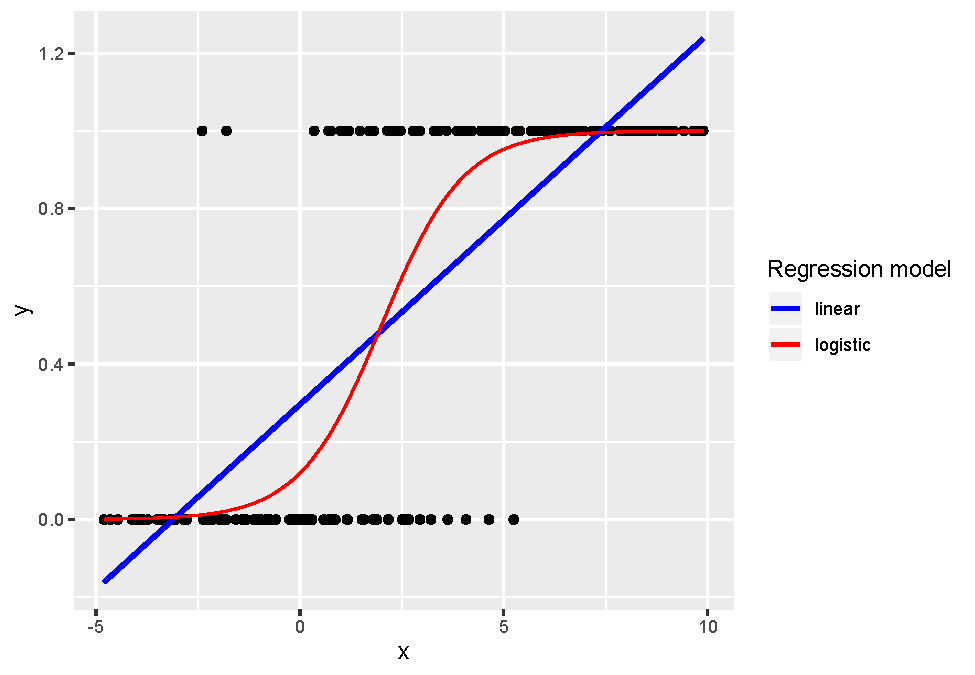
\includegraphics[width=0.6\linewidth]{bookdown-bysh_files/figure-latex/OLSlogistic-1} 

}

\caption{Linear vs. Logistic regression models for binary response data.}\label{fig:OLSlogistic}
\end{figure}

Figure \ref{fig:OLSlogistic} illustrates a data set with a binary (0 or 1) response (Y) and a single continuous predictor (X). The blue line is a linear regression fit with least squares to model the probability of a success (Y=1) for a given value of X. With a binary response, the line doesn't fit the data well, and it produces predicted probabilities below 0 and above 1. On the other hand, the logistic regression fit (red curve) with its typical ``S'' shape follows the data closely and always produces predicted probabilities between 0 and 1. For these and several other reasons detailed in this chapter, we will focus on the following model for logistic regression with binary or binomial responses:

\begin{equation*}
log(\frac{p_i}{1-p_i})=\beta_0+\beta_1 x_i
\end{equation*}
where the observed values \(Y_i \sim\) binomial with \(p=p_i\) for a given \(x_i\) and \(n=1\) for binary responses.

\hypertarget{case-studies-overview-1}{%
\section{Case Studies Overview}\label{case-studies-overview-1}}

We consider three case studies in this chapter. The first two involve binomial responses (Soccer Goalkeepers and Reconstructing Alabama), while the last case uses a binary response (Trying to Lose Weight). Even though binary responses are much more common, their models have a very similar form to binomial responses, so the first two case studies will illustrate important principles that also apply to the binary case. Here are the statistical concepts you will encounter for each Case Study.

The soccer goalkeeper data can be written in the form of a 2 \(\times\) 2 table. This example is used to describe some of the underlying theory for logistic regression. We demonstrate how binomial probability mass functions (pmfs) can be written in one parameter exponential family form, from which we can identify the canonical link as in Chapter \ref{ch-glms}. Using the canonical link, we write a Generalized Linear Model for binomial counts and determine corresponding MLEs for model coefficients. Interpretation of the estimated parameters involves a fundamental concept, the odds ratio.

The Reconstructing Alabama case study is another binomial example which introduces the notion of deviances, which are used to compare and assess models. Thus, we will investigate hypothesis tests and confidence intervals, including issues of interaction terms, overdispersion, and lack of fit. We will also check the assumptions of logistic regression using empirical logit plots and deviance residuals.

The last case study addresses why teens try to lose weight. Here the response is a binary variable which allows us to analyze individual level data. The analysis builds on concepts from the previous sections in the context of a random sample from CDC's Youth Risk Behavior Survey (YRBS).

\hypertarget{case-study-soccer-goalkeepers}{%
\section{Case Study: Soccer Goalkeepers}\label{case-study-soccer-goalkeepers}}

Does the probability of a save in a soccer match depend upon whether the goalkeeper's team is behind or not? \citet{Roskes2011} looked at penalty kicks in the men's World Cup soccer championships from 1982 - 2010, and they assembled data on 204 penalty kicks during shootouts. The data for this study is summarized in Table \ref{tab:table1chp6}.

\begin{table}

\caption{\label{tab:table1chp6}Soccer goalkeepers' penalty kick saves when their team is and is not behind.  Source: Roskes et al. 2011 Psychological Science}
\centering
\begin{tabular}[t]{lrrr}
\toprule
  & Saves & Scores & Total\\
\midrule
Behind & 2 & 22 & 24\\
Not Behind & 39 & 141 & 180\\
Total & 41 & 163 & 204\\
\bottomrule
\end{tabular}
\end{table}

\hypertarget{modeling-odds}{%
\subsection{Modeling Odds}\label{modeling-odds}}

Odds are one way to quantify a goalkeeper's performance. Here the odds that a goalkeeper makes a save when his team is behind is 2 to 22 or 0.09 to 1. Or equivalently, the odds that a goal is scored on a penalty kick is 22 to 2 or 11 to 1. An odds of 11 to 1 tells you that a shooter whose team is ahead will score 11 times for every 1 shot that the goalkeeper saves. When the goalkeeper's team is not behind the odds a goal is scored is 141 to 39 or 3.61 to 1. We see that the odds of a goal scored on a penalty kick are better when the goalkeeper's team is behind than when it is not behind (i.e., better odds of scoring for the shooter when the shooter's team is ahead). We can compare these odds by calculating the \textbf{odds ratio} \index{odds ratio} (OR), 11/3.61 or 3.05, which tells us that the \emph{odds} of a successful penalty kick are 3.05 times higher when the shooter's team is leading.

In our example, it is also possible to estimate the probability of a goal, \(p\), for either circumstance. When the goalkeeper's team is behind, the probability of a successful penalty kick is \(p\) = 22/24 or 0.833. We can see that the ratio of the probability of a goal scored divided by the probability of no goal is \((22/24)/(2/24)=22/2\) or 11, the odds we had calculated above. The same calculation can be made when the goalkeeper's team is not behind. In general, we now have several ways of finding the odds of success under certain circumstances:

\[\textrm{Odds} = \frac{\# \textrm{successes}}{\# \textrm{failures}}=
\frac{\# \textrm{successes}/n}{\# \textrm{failures}/n}=
\frac{p}{1-p}.\]

\hypertarget{logistic-regression-models-for-binomial-responses}{%
\subsection{Logistic Regression Models for Binomial Responses}\label{logistic-regression-models-for-binomial-responses}}

We would like to model the odds of success, however odds are strictly positive. Therefore, similar to modeling log(\(\lambda\)) in Poisson regression, which allowed the response to take on values from \(-\infty\) to \(\infty\), we will model the log(odds), the \textbf{logit}\index{logit}, in logistic regression. Logits will be suitable for modeling with a linear function of the predictors:

\begin{equation*}
\log\left(\frac{p}{1 - p}\right)=\beta_0+\beta_1X 
 \end{equation*}
Models of this form are referred to as \textbf{binomial regression models},\index{binomial logistic regression} or more generally as \textbf{logistic regression models}. \index{logistic regression} Here we provide intuition for using and interpreting logistic regression models, and then in the short optional section that follows, we present rationale for these models using GLM theory.

In our example we could define \(X=0\) for not behind and \(X=1\) for behind and fit the model:

\begin{equation}
\log\left(\frac{p_X}{1-p_X}\right)=\beta_0 +\beta_1X
\label{eq:logitXform}
\end{equation}
where \(p_X\) is the probability of a successful penalty kick given \(X\).

So, based on this model, the log odds of a successful penalty kick when the goalkeeper's team is not behind is:

\[
\log\left(\frac{p_0}{1-p_0}\right) =\beta_0 \nonumber,
\]
and the log odds when the team is behind is:

\[
\log\left(\frac{p_1}{1-p_1}\right)=\beta_0+\beta_1. \nonumber
\]

We can see that \(\beta_1\) is the difference between the log odds of a successful penalty kick between games when the goalkeeper's team is behind and games when the team is not behind. Using rules of logs:

\begin{equation*}
\beta_1 = (\beta_0 + \beta_1) - \beta_0 = 
\log\left(\frac{p_1}{1-p_1}\right) - \log\left(\frac{p_0}{1-p_0}\right) =
\log\left(\frac{p_1/(1-p_1)}{p_0/{(1-p_0)}}\right).
\end{equation*}

Thus \(e^{\beta_1}\) is the ratio of the odds of scoring when the goalkeeper's team is not behind compared to scoring when the team is behind. In general, \emph{exponentiated coefficients in logistic regression are odds ratios (OR)}. A general interpretation of an OR is the odds of success for group A compared to the odds of success for group B---how many times greater the odds of success are in group A compared to group B.

The logit model (Equation \eqref{eq:logitXform}) can also be re-written in a \textbf{probability form}:

\begin{equation*} 
p_X=\frac{e^{\beta_0+\beta_1X}}{1+e^{\beta_0+\beta_1X}}
\end{equation*}
which can be re-written for games when the goalkeeper's team is behind as:

\begin{equation} 
p_1=\frac{e^{\beta_0+\beta_1}}{1+e^{\beta_0+\beta_1}}  
\label{eq:pBehindform}
\end{equation}
and for games when the goalkeeper's team is not behind as:

\begin{equation} 
p_0=\frac{e^{\beta_0}}{1+e^{\beta_0}}
\label{eq:pNotBehindform}
\end{equation}

We use likelihood methods to estimate \(\beta_0\) and \(\beta_1\). As we had done in Chapter \ref{ch-beyondmost}, we can write the likelihood for this example in the following form:

\[\Lik(p_1, p_0) = {28 \choose 22}p_1^{22}(1-p_1)^{2}
{180 \choose 141}p_0^{141}(1-p_0)^{39}\]

Our interest centers on estimating \(\hat{\beta_0}\) and \(\hat{\beta_1}\), not \(p_1\) or \(p_0\). So we replace \(p_1\) in the likelihood with an expression for \(p_1\) in terms of \(\beta_0\) and \(\beta_1\) as in Equation \eqref{eq:pBehindform}. Similarly, \(p_0\) in Equation \eqref{eq:pNotBehindform} involves only \(\beta_0\). After removing constants, the new likelihood looks like:

\begin{equation*}
\begin{gathered}
    \Lik(\beta_0,\beta_1) \propto \\
    \left( \frac{e^{\beta_0+\beta_1}}{1+e^{\beta_0+\beta_1}}\right)^{22}\left(1- \frac{e^{\beta_0+\beta_1}}{1+e^{\beta_0+\beta_1}}\right)^{2}
    \left(\frac{e^{\beta_0}}{1+e^{\beta_0}}\right)^{141}\left(1-\frac{e^{\beta_0}}{1+e^{\beta_0}}\right)^{39}
\end{gathered}
\end{equation*}

Now what? Fitting the model means finding estimates of \(\beta_0\) and \(\beta_1\), but familiar methods from calculus for maximizing the likelihood don't work here. Instead, we consider all possible combinations of \(\beta_0\) and \(\beta_1\). That is, we will pick that pair of values for \(\beta_0\) and \(\beta_1\) that yield the largest likelihood for our data. Trial and error to find the best pair is tedious at best, but more efficient numerical methods are available. The MLEs for the coefficients in the soccer goalkeeper study are \(\hat{\beta_0}= 1.2852\) and \(\hat{\beta_1}=1.1127\).

Exponentiating \(\hat{\beta_1}\) provides an estimate of the odds ratio (the odds of scoring when the goalkeeper's team is behind compared to the odds of scoring when the team is not behind) of 3.04, which is consistent with our calculations using the 2 \(\times\) 2 table. We estimate that the odds of scoring when the goalkeeper's team is behind is over 3 times that of when the team is not behind or, in other words, the odds a shooter is successful in a penalty kick shootout are 3.04 times higher when his team is leading.
\vspace{5mm}

\textbf{Time out for study discussion (Optional).}

\begin{itemize}
\item
  Discuss the following quote from the study abstract: ``Because penalty takers shot at the two sides of the goal equally often, the goalkeepers' right-oriented bias was dysfunctional, allowing more goals to be scored.''
\item
  Construct an argument for why the greater success observed when the goalkeeper's team was behind might be better explained from the shooter's perspective.
\end{itemize}

Before we go on, you may be curious as to why there is \emph{no error term} in our model statements for logistic or Poisson regression. One way to look at it is to consider that all models describe how observed values are generated. With the logistic model we assume that the observations are generated as a binomial random variables. Each observation or realization of \(Y\) = number of successes in \(n\) independent and identical trials with a probability of success on any one trial of \(p\) is produced by \(Y \sim \textrm{Binomial}(n,p)\). So the randomness in this model is not introduced by an added error term but rather by appealing to a Binomial probability distribution, where variability depends only on \(n\) and \(p\) through \(\textrm{Var}(Y)=np(1-p)\), and where \(n\) is usually considered fixed and \(p\) the parameter of interest.

\hypertarget{theoretical-rationale-for-logistic-regression-models-optional}{%
\subsection{Theoretical rationale for logistic regression models (Optional)}\label{theoretical-rationale-for-logistic-regression-models-optional}}

Recall from Chapter \ref{ch-glms} that generalized linear models (GLMs) \index{generalized linear models (GLMs)} are a way in which to model a variety of different types of responses. In this chapter, we apply the general results of GLMs to the specific application of binomial responses. Let \(Y\) = the number scored out of \(n\) penalty kicks. The parameter, \(p\), is the probability of a score on a single penalty kick. Recall that the theory of GLMs is based on the unifying notion of the one-parameter exponential family form:

\begin{equation*}
f(y;\theta)=e^{[a(y)b(\theta)+c(\theta)+d(y)]}
\end{equation*}
To see that we can apply the general approach of GLMs \index{generalized linear models (GLMs)} to binomial responses, we first write an expression for the probability of a binomial response and then use a little algebra to rewrite it until we can demonstrate that it, too, can be written in one-parameter exponential family form with \(\theta = p\). This will provide a way in which to specify the canonical link and the form for the model. Additional theory allows us to deduce the mean, standard deviation, and more from this form.

If \(Y\) follows a binomial distribution with \(n\) trials and probability of success \(p\), we can write:

\begin{align*}
P(Y=y)&= \binom{n}{y}p^y(1-p)^{(n-y)} \\
      &=e^{y\log(p) + (n-y)\log(1-p) + \log\binom{n}{y}}
\end{align*}
However, this probability mass function is not quite in one parameter exponential family form. Note that there are two terms in the exponent which consist of a product of functions of \(y\) and \(p\). So more simplification is in order:

\begin{equation*}
P(Y=y) = e^{y\log\left(\frac{p}{1-p}\right) + n\log(1-p)+ \log\binom{n}{y}}
\end{equation*}
Don't forget to consider the support; we must make sure that the set of possible values for this response is not dependent upon \(p\). For fixed \(n\) and any value of \(p\), \(0<p<1\), all integer values from \(0\) to \(n\) are possible, so the support is indeed independent of \(p\).

The one parameter exponential family form for binomial responses shows that the canonical link is \(\log\left(\frac{p}{1-p}\right)\). Thus, GLM theory suggests that constructing a model using the logit, the log odds of a score, as a linear function of covariates is a reasonable approach.

\hypertarget{case-study-reconstructing-alabama}{%
\section{Case Study: Reconstructing Alabama}\label{case-study-reconstructing-alabama}}

This case study demonstrates how wide-ranging applications of statistics can be. Many would not associate statistics with historical research, but this case study shows that it can be done. US Census data from 1870 helped historian Michael Fitzgerald of St.~Olaf College gain insight into important questions about how railroads were supported during the Reconstruction Era.

In a paper entitled ``Reconstructing Alabama: Reconstruction Era Demographic and Statistical Research,'' Ben Bayer performs an analysis of data from 1870 to explain influences on voting on referendums related to railroad subsidies \citep{Bayer2011}. Positive votes are hypothesized to be inversely proportional to the distance a voter is from the proposed railroad, but the racial composition of a community (as measured by the percentage of blacks) is hypothesized to be associated with voting behavior as well. Separate analyses of three counties in Alabama---Hale, Clarke, and Dallas---were performed; we discuss Hale County here. This example differs from the soccer example in that it includes continuous covariates. Was voting on railroad referenda related to distance from the proposed railroad line and the racial composition of a community?

\hypertarget{data-organization-2}{%
\subsection{Data Organization}\label{data-organization-2}}

The unit of observation for this data is a community in Hale County. We will focus on the following variables from \texttt{RR\_Data\_Hale.csv} collected for each community (see Table \ref{tab:table2chp6}):

\begin{itemize}
\item
  \texttt{pctBlack} = the percentage of blacks in the community
\item
  \texttt{distance} = the distance, in miles, the proposed railroad is from the community
\item
  \texttt{YesVotes} = the number of ``Yes'' votes in favor of the proposed railroad line (our primary response variable)
\item
  \texttt{NumVotes} = total number of votes cast in the election
\end{itemize}

\begin{table}

\caption{\label{tab:table2chp6}Sample of the data for the Hale County, Alabama, railroad subsidy vote.}
\centering
\begin{tabular}[t]{llrrr}
\toprule
community & pctBlack & distance & YesVotes & NumVotes\\
\midrule
Carthage & 58.4 & 17 & 61 & 110\\
Cederville & 92.4 & 7 & 0 & 15\\
Greensboro & 59.4 & 0 & 1790 & 1804\\
Havana & 58.4 & 12 & 16 & 68\\
\bottomrule
\end{tabular}
\end{table}

\hypertarget{exploratory-analyses}{%
\subsection{Exploratory Analyses}\label{exploratory-analyses}}

We first look at a coded scatterplot to see our data. Figure \ref{fig:coded} portrays the relationship between \texttt{distance} and \texttt{pctBlack} coded by the \texttt{InFavor} status (whether a community supported the referendum with over 50\% Yes votes). From this scatterplot, we can see that all of the communities in favor of the railroad referendum are over 55\% black, and all of those opposed are 7 miles or farther from the proposed line. The overall percentage of voters in Hale County in favor of the railroad is 87.9\%.

\begin{figure}

{\centering 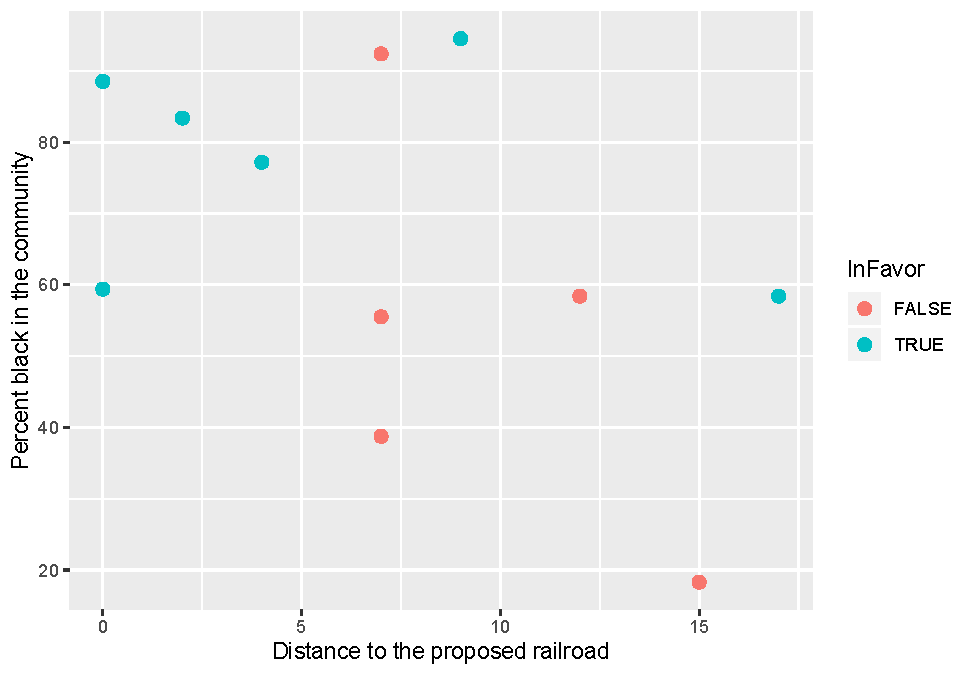
\includegraphics[width=0.6\linewidth]{bookdown-bysh_files/figure-latex/coded-1} 

}

\caption{ Scatterplot of distance from a proposed rail line and percent black in the community coded by whether the community was in favor of the referendum or not.}\label{fig:coded}
\end{figure}

Recall that a model with two covariates has the form:

\[\log(\textrm{odds}) = \log\left(\frac{p}{1-p}\right) = \beta_0+\beta_1X_1+\beta_2X_2.\]
where \(p\) is the proportion of Yes votes in a community. In logistic regression, we expect the logits to be a linear function of \(X\), the predictors. To assess the linearity assumption, we construct \textbf{empirical logit plots} \index{empirical logit plot}, where ``empirical'' means ``based on sample data.'' Empirical logits are computed for each community by taking \(\log\left(\frac{\textrm{number of successes}}{\textrm{number of failures}}\right)\). In Figure \ref{fig:emplogits}, we see that the plot of empirical logits versus distance produces a plot that looks linear, as needed for the logistic regression assumption. In contrast, the empirical logits by percent black reveal that Greensboro deviates quite a bit from the otherwise linear pattern; this suggests that Greensboro is an outlier and possibly an influential point. Greensboro has 99.2\% voting yes with only 59.4\% black.

\begin{figure}

{\centering 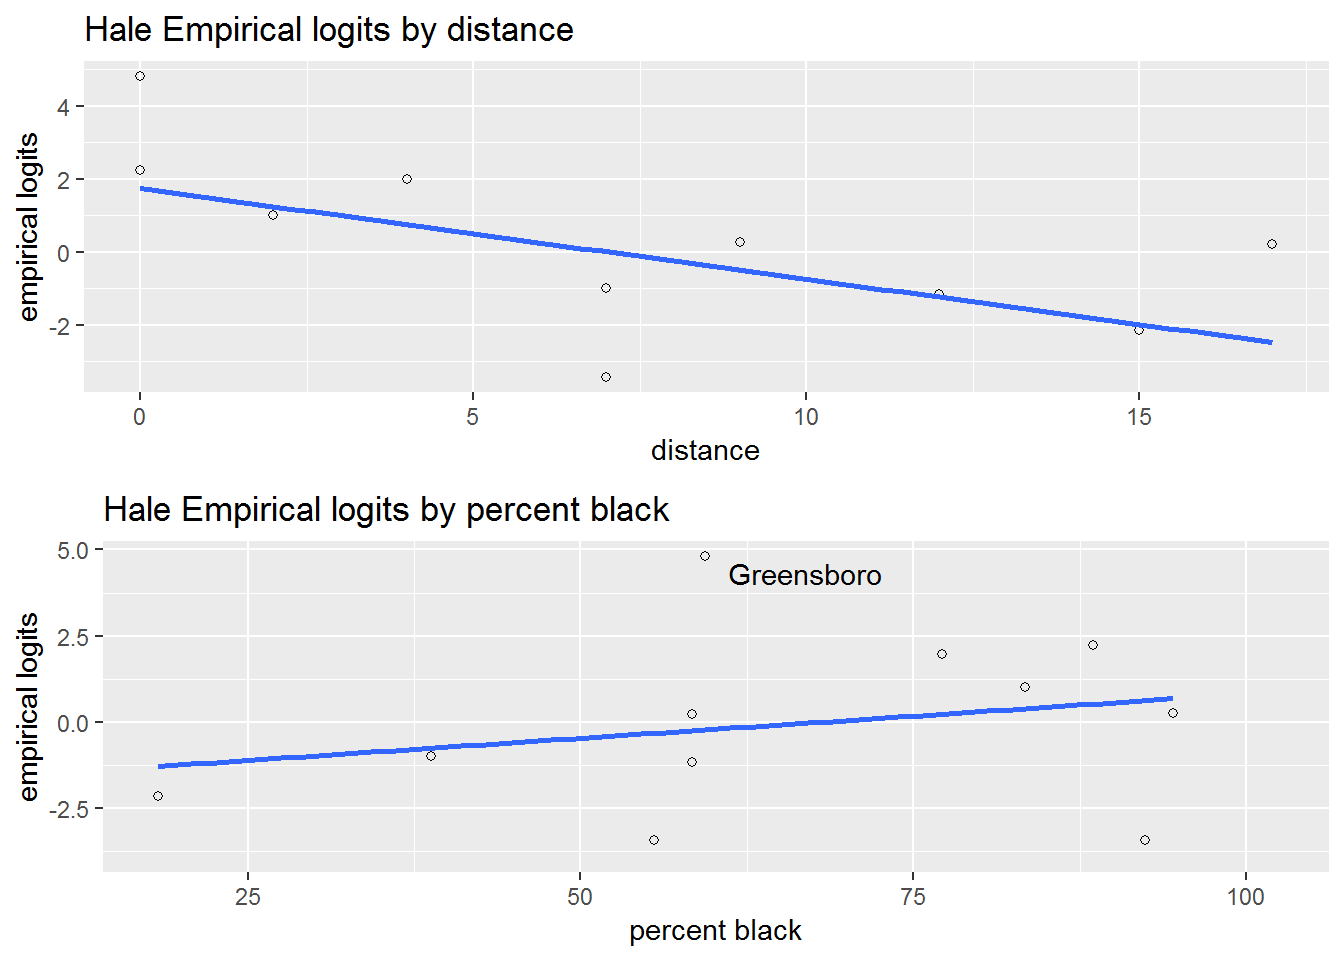
\includegraphics[width=0.6\linewidth]{bookdown-bysh_files/figure-latex/emplogits-1} 

}

\caption{Empirical logit plots for the Railroad Referendum data.}\label{fig:emplogits}
\end{figure}

In addition to examining how the response correlates with the predictors, it is a good idea to determine whether the predictors correlate with one another. Here the correlation between distance and percent black is negative and moderately strong with \(r = -0.49\). We'll watch to see if the correlation affects the stability of our odds ratio estimates.

\hypertarget{initial-models-1}{%
\subsection{Initial Models}\label{initial-models-1}}

The first model includes only one covariate, distance.

\begin{Shaded}
\begin{Highlighting}[]
\CommentTok{# Model with just distance}
\NormalTok{model.HaleD <-}\StringTok{ }\KeywordTok{glm}\NormalTok{(}\KeywordTok{cbind}\NormalTok{(YesVotes, NumVotes }\OperatorTok{-}\StringTok{ }\NormalTok{YesVotes) }\OperatorTok{~}
\StringTok{    }\NormalTok{distance, }\DataTypeTok{family =}\NormalTok{ binomial, }\DataTypeTok{data =}\NormalTok{ rrHale.df)}
\CommentTok{# alternative expression}
\NormalTok{model.HaleD.alt <-}\StringTok{ }\KeywordTok{glm}\NormalTok{(YesVotes }\OperatorTok{/}\StringTok{ }\NormalTok{NumVotes }\OperatorTok{~}\StringTok{ }\NormalTok{distance, }
    \DataTypeTok{weights =}\NormalTok{ NumVotes, }\DataTypeTok{family =}\NormalTok{ binomial, }\DataTypeTok{data =}\NormalTok{ rrHale.df)}
\end{Highlighting}
\end{Shaded}

\begin{verbatim}
##             Estimate Std. Error z value   Pr(>|z|)
## (Intercept)   3.3093    0.11313   29.25 4.268e-188
## distance     -0.2876    0.01302  -22.08 4.447e-108
\end{verbatim}

\begin{verbatim}
##  Residual deviance =  318.4  on  9 df 
##  Dispersion parameter =  1
\end{verbatim}

Our estimated binomial regression model is:

\[\log\left(\frac{\hat{p}_i}{1-\hat{p}_i}\right)=3.309-0.288 \textrm{distance}_i\]
where \(\hat{p}_i\) is the estimated proportion of Yes votes in community \(i\). The estimated odds ratio for distance, that is the exponentiated coefficient for distance, in this model is \(e^{-0.288}=0.750\). It can be interpreted as follows: for each additional mile from the proposed railroad, the support (odds of a Yes vote) declines by 25.0\%.

The covariate \texttt{pctBlack} is then added to the first model.

\begin{Shaded}
\begin{Highlighting}[]
\NormalTok{model.HaleBD <-}\StringTok{ }\KeywordTok{glm}\NormalTok{(}\KeywordTok{cbind}\NormalTok{(YesVotes, NumVotes }\OperatorTok{-}\StringTok{ }\NormalTok{YesVotes) }\OperatorTok{~}
\StringTok{  }\NormalTok{distance }\OperatorTok{+}\StringTok{ }\NormalTok{pctBlack, }\DataTypeTok{family =}\NormalTok{ binomial, }\DataTypeTok{data =}\NormalTok{ rrHale.df)}
\end{Highlighting}
\end{Shaded}

\begin{verbatim}
##             Estimate Std. Error z value   Pr(>|z|)
## (Intercept)  4.22202   0.296963  14.217  7.155e-46
## distance    -0.29173   0.013100 -22.270 7.236e-110
## pctBlack    -0.01323   0.003897  -3.394  6.881e-04
\end{verbatim}

\begin{verbatim}
##  Residual deviance =  307.2  on  8 df 
##  Dispersion parameter =  1
\end{verbatim}

Despite the somewhat strong negative correlation between percent black and distance, the estimated odds ratio for distance remains approximately the same in this new model (OR \(= e^{-0.29} = 0.747\)); controlling for percent black does little to change our estimate of the effect of distance. For each additional mile from the proposed railroad, odds of a Yes vote declines by 25.3\% after adjusting for the racial composition of a community. We also see that, for a fixed distance from the proposed railroad, the odds of a Yes vote declines by 1.3\% (OR \(= e^{-.0132} = .987\)) for each additional percent black in the community.

\hypertarget{sec-logisticInf}{%
\subsection{Tests for significance of model coefficients}\label{sec-logisticInf}}

Do we have statistically significant evidence that support for the railroad referendum decreases with higher proportions of black residents in a community, after accounting for the distance a community is from the railroad line? As discussed in Section \ref{cs-philippines} with Poisson regression, there are two primary approaches to testing signficance of model coefficients: \textbf{Drop-in-deviance test to compare models} \index{drop-in-deviance test} and \textbf{Wald test for a single coefficient} \index{Wald-type test}.

With our larger model given by \(\log\left(\frac{p_i}{1-p_i}\right) = \beta_0+\beta_1\textrm{distance}_i+\beta_2\textrm{pctBlack}_i\), the Wald test produces a highly significant p-value (\(Z=\frac{-0.0132}{0.0039}= -3.394\), \(p=.00069\)) indicating significant evidience that support for the railroad referendum decreases with higher proportions of black residents in a community, after adjusting for the distance a community is from the railroad line.

The drop in deviance test would compare the larger model above to the reduced model \(\log\left(\frac{p_i}{1-p_i}\right) = \beta_0+\beta_1\textrm{distance}_i\) by comparing residual deviances from the two models.

\begin{Shaded}
\begin{Highlighting}[]
\NormalTok{drop_in_dev <-}\StringTok{ }\KeywordTok{anova}\NormalTok{(model.HaleD, model.HaleBD, }\DataTypeTok{test =} \StringTok{"Chisq"}\NormalTok{)}
\end{Highlighting}
\end{Shaded}

\begin{verbatim}
  ResidDF ResidDev Deviance Df      pval
1       9    318.4       NA NA        NA
2       8    307.2    11.22  1 0.0008083
\end{verbatim}

The drop-in-deviance test statistic is \(318.44 - 307.22 = 11.22\) on \(9 - 8 = 1\) df, producing a p-value of .00081, in close agreement with the Wald test.

A third approach to determining significance of \(\beta_2\) would be to generate a 95\% confidence interval and then checking if 0 falls within the interval or, equivalently, if 1 falls within a 95\% confidence interval for \(e^{\beta_2}.\) The next section describes two approaches to producing a confidence interval for coefficients in logistic regression models.

\hypertarget{confidence-intervals-for-model-coefficients}{%
\subsection{Confidence intervals for model coefficients}\label{confidence-intervals-for-model-coefficients}}

Since the Wald statistic follows a normal distribution with \(n\) large, we could generate a Wald-type (normal-based) confidence interval \index{Wald-type confidence interval} for \(\beta_2\) using:

\[\hat\beta_2 \pm 1.96\cdot\textrm{SE}(\hat\beta_2)\]
and then exponentiating endpoints if we prefer a confidence interval for the odds ratio \(e^{\beta_2}\). In this case,

\begin{align*}
95\% \textrm{ CI for } \beta_2 &= \hat{\beta}_2 \pm 1.96 \cdot \textrm{SE}(\hat{\beta}_2) \\
                               &= -0.0132 \pm 1.96 \cdot 0.0039 \\
                               &= -0.0132 \pm 0.00764 \\
                               &= (-0.0208, -0.0056) \\
95\% \textrm{ CI for } e^{\beta_2} &= (e^{-0.0208}, e^{-0.0056}) \\
                                   &= (.979, .994) \\
95\% \textrm{ CI for } e^{10\beta_2} &= (e^{-0.208}, e^{-0.056}) \\
                                      &= (.812, .946)
\end{align*}

Thus, we can be 95\% confident that a 10\% increase in the proportion of black residents is associated with a 5.4\% to 18.8\% decrease in the odds of a Yes vote for the railroad referendum after controlling for distance. This same relationship could be expressed as (a) between a 0.6\% and a 2.1\% decrease in odds for each 1\% increase in the black population, or (b) between a 5.7\% (\(1/e^{-.056}\)) and a 23.1\% (\(1/e^{-.208}\)) increase in odds for each 10\% decrease in the black population, after adjusting for distance. Of course, with \(n=11\), we should be cautious about relying on a Wald-type interval in this example.

Another approach available in R is the \textbf{profile likelihood method} \index{profile likelihood}, similar to Section \ref{cs-philippines}.

\begin{Shaded}
\begin{Highlighting}[]
\KeywordTok{exp}\NormalTok{(}\KeywordTok{confint}\NormalTok{(model.HaleBD))}
\end{Highlighting}
\end{Shaded}

\begin{verbatim}
              2.5 %   97.5 %
(Intercept) 38.2285 122.6116
distance     0.7276   0.7660
pctBlack     0.9794   0.9945
\end{verbatim}

In the model with \texttt{distance} and \texttt{pctBlack}, the profile likelihood 95\% confidence interval for \(e^{\beta_2}\) is (.979, .994), which is approximately equal to the Wald-based interval despite the small sample size. We can also confirm the statistically significant association between percent black and odds of voting Yes (after controlling for distance), because 1 is not a plausible value of \(e^{\beta_2}\) (where an odds ratio of 1 would imply that the odds of voting Yes do not change with percent black).

\hypertarget{testing-for-goodness-of-fit}{%
\subsection{Testing for goodness of fit}\label{testing-for-goodness-of-fit}}

As in Section \ref{sec-PoisGOF}, we can evaluate the goodness of fit for our model by comparing the residual deviance (307.22) to a \(\chi^2\) distribution with \(n-p\) (8) degrees of freedom.

\begin{Shaded}
\begin{Highlighting}[]
\DecValTok{1}\OperatorTok{-}\KeywordTok{pchisq}\NormalTok{(}\FloatTok{307.2173}\NormalTok{, }\DecValTok{8}\NormalTok{)  }\CommentTok{# Goodness of fit test}
\end{Highlighting}
\end{Shaded}

\begin{verbatim}
[1] 0
\end{verbatim}

The model with \texttt{pctBlack} and \texttt{distance} has statistically significant evidence of lack of fit (\(p<.001\)).

Similar to the Poisson regression models, this lack of fit \index{lack of fit} could result from (a) missing covariates, (b) outliers, or (c) overdispersion. We will first attempt to address (a) by fitting a model with an interaction between distance and percent black, to determine whether the effect of racial composition differs based on how far a community is from the proposed railroad.

\begin{Shaded}
\begin{Highlighting}[]
\NormalTok{model.HaleBxD <-}\StringTok{ }\KeywordTok{glm}\NormalTok{(}\KeywordTok{cbind}\NormalTok{(YesVotes, NumVotes }\OperatorTok{-}\StringTok{ }\NormalTok{YesVotes) }\OperatorTok{~}
\StringTok{  }\NormalTok{distance }\OperatorTok{+}\StringTok{ }\NormalTok{pctBlack }\OperatorTok{+}\StringTok{ }\NormalTok{distance}\OperatorTok{:}\NormalTok{pctBlack, }
  \DataTypeTok{family =}\NormalTok{ binomial, }\DataTypeTok{data =}\NormalTok{ rrHale.df)}
\end{Highlighting}
\end{Shaded}

\begin{verbatim}
##                    Estimate Std. Error z value
## (Intercept)        7.550902  0.6383697  11.828
## distance          -0.614005  0.0573808 -10.701
## pctBlack          -0.064731  0.0091723  -7.057
## distance:pctBlack  0.005367  0.0008984   5.974
##                    Pr(>|z|)
## (Intercept)       2.783e-32
## distance          1.012e-26
## pctBlack          1.698e-12
## distance:pctBlack 2.321e-09
\end{verbatim}

\begin{verbatim}
##  Residual deviance =  274.2  on  7 df 
##  Dispersion parameter =  1
\end{verbatim}

\begin{Shaded}
\begin{Highlighting}[]
\NormalTok{drop_in_dev <-}\StringTok{ }\KeywordTok{anova}\NormalTok{(model.HaleBD, model.HaleBxD, }
                     \DataTypeTok{test =} \StringTok{"Chisq"}\NormalTok{)}
\end{Highlighting}
\end{Shaded}

\begin{verbatim}
  ResidDF ResidDev Deviance Df      pval
1       8    307.2       NA NA        NA
2       7    274.2    32.98  1 9.294e-09
\end{verbatim}

We have statistically significant evidence (Wald test: \(Z = 5.974, p<.001\); Drop in deviance test: \(\chi^2=32.984, p<.001\)) that the effect of the proportion of the community that is black on the odds of voting Yes depends on the distance of the community from the proposed railroad.

To interpret the interaction coefficient in context, we will compare two cases: one where a community is right on the proposed railroad (\texttt{distance} = 0), and the other where the community is 15 miles away (\texttt{distance} = 15). The significant interaction implies that the effect of \texttt{pctBlack} should differ in these two cases. In the first case, the coefficient for \texttt{pctBlack} is -0.0647, while in the second case, the relevant coefficient is \(-0.0647+15(.00537) = 0.0158\). Thus, for a community right on the proposed railroad, a 1\% increase in percent black is associated with a 6.3\% (\(e^{-.0647}=.937\)) decrease in the odds of voting Yes, while for a community 15 miles away, a 1\% increase in percent black is associated with a (\(e^{.0158}=1.016\)) 1.6\% \emph{increase} in the odds of voting Yes. A significant interaction term doesn't always imply a change in the direction of the association, but it does here.

Because our interaction model still exhibits lack of fit (residual deviance of 274.23 on just 7 df), and because we have used the covariates at our disposal, we will assess this model for potential outliers and overdispersion by examining the model's residuals.

\hypertarget{residuals-for-binomial-regression}{%
\subsection{Residuals for Binomial Regression}\label{residuals-for-binomial-regression}}

With LLSR, residuals were used to assess model assumptions and identify outliers. For binomial regression, two different types of residuals are typically used. One residual, the \textbf{Pearson residual} \index{Pearson residuals}, has a form similar to that used with LLSR. Specifically, the Pearson residual is calculated using:

\begin{equation*}
\textrm{Pearson residual}_i = \frac{\textrm{actual count}-\textrm{predicted count}}{\textrm{SD of count}} =
\frac{Y_i-m_i\hat{p_i}}{\sqrt{m_i\hat{p_i}(1-\hat{p_i})}}
\end{equation*}
where \(m_i\) is the number of trials for the \(i^{th}\) observation and \(\hat{p}_i\) is the estimated probability of success for that same observation.

A \textbf{deviance residual} \index{deviance residuals} is an alternative residual for binomial regression based on the discrepancy between the observed values and those estimated using the likelihood.
A deviance residual can be calculated for each observation using:

\begin{equation*}
\textrm{d}_i = 
\textrm{sign}(Y_i-m_i\hat{p_i})\sqrt{2[Y_i \log\left(\frac{Y_i}{m_i \hat{p_i}}\right)+
(m_i - Y_i) \log\left(\frac{m_i - Y_i}{m_i - m_i \hat{p_i}}\right)]}
\end{equation*}

When the number of trials is large for all of the observations and the models are appropriate, both sets of residuals should follow a standard normal distribution.

The sum of the individual deviance residuals is referred to as the \textbf{deviance} or \textbf{residual deviance} \index{residual deviance}. The residual deviance is used to assess the model. As the name suggests, a model with a small deviance is preferred. In the case of binomial regression, when the denominators, \(m_i\), are large and a model fits, the residual deviance follows a \(\chi^2\) distribution with \(n-p\) degrees of freedom (the residual degrees of freedom). Thus for a good fitting model the residual deviance should be approximately equal to its corresponding degrees of freedom. When binomial data meets these conditions, the deviance can be used for a goodness-of-fit test. The p-value for lack-of-fit is the proportion of values from a \(\chi_{n-p}^2\) that are greater than the observed residual deviance.

We begin a residual analysis of our interaction model by plotting the residuals against the fitted values in Figure \ref{fig:resid}. This kind of plot for binomial regression would produce two linear trends with similar negative slopes if there were equal sample sizes \(m_i\) for each observation.

\begin{figure}

{\centering 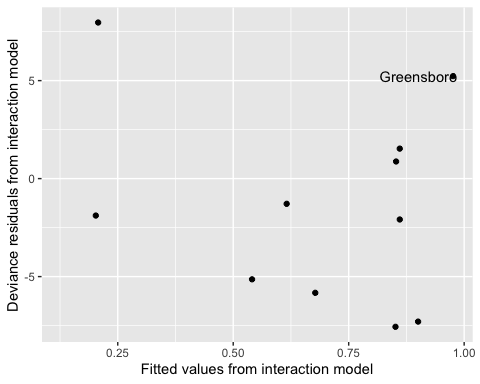
\includegraphics[width=0.6\linewidth]{bookdown-bysh_files/figure-latex/resid-1} 

}

\caption{Fitted values by residuals for the interaction model for the Railroad Referendum data.}\label{fig:resid}
\end{figure}

From this residual plot, Greensboro does not stand out as an outlier. If it did, we could remove Greensboro and refit our interaction model, checking to see if model coefficients changed in a noticeable way. Instead, we will continue to include Greensboro in our modeling efforts. Because the large residual deviance cannot be explained by outliers, and given we have included all of the covariates at hand as well as an interaction term, the observed binomial counts are likely overdispersed. This means that they exhibit more variation than the model would suggest, and we must consider ways to handle this overdispersion.

\hypertarget{sec-logOverdispersion}{%
\subsection{Overdispersion}\label{sec-logOverdispersion}}

Similarly to Poisson regression we can adjust for overdispersion \index{overdispersion} in binomial regression. With overdispersion there is \textbf{extra-binomial variation} \index{extra-binomial variation}, so the actual variance will be greater than the variance of a binomial variable, \(np(1-p)\). One way to adjust for overdispersion is to estimate a multiplier (dispersion parameter), \(\hat{\phi}\), for the variance that will inflate it and reflect the reduction in the amount of information we would otherwise have with independent observations. We used a similar approach to adjust for overdispersion in a Poisson regression model in Section \ref{sec-overdispPois}, and we will use the same estimate here: \(\hat\phi=\frac{\sum(\textrm{Pearson residuals})^2}{n-p}\).

When overdispersion is adjusted for in this way, we can no longer use maximum likelihood to fit our regression model; instead we use a quasilikelihood approach \index{quasilikelihood}. Quasilikelihood is similar to likelihood-based inference, but because the model uses the dispersion parameter, it is not a binomial model with a true likelihood (we call it \textbf{quasibinomial} \index{quasibinomial}). R offers quasilikelihood as an option when model fitting. The quasilikelihood approach will yield the same coefficient point estimates as maximum likelihood; however, the variances will be larger in the presence of overdispersion (assuming \(\phi>1\)). We will see other ways in which to deal with overdispersion and clusters in the remaining chapters in the book, but the following describes how overdispersion is accounted for using \(\hat{\phi}\):
\vspace{5mm}

\textbf{Summary: Accounting for Overdispersion}

\begin{itemize}
\tightlist
\item
  Use the dispersion parameter \(\hat\phi=\frac{\sum(\textrm{Pearson residuals})^2}{n-p}\) to inflate standard errors of model coefficients
\item
  Wald test statistics: multiply the standard errors by \(\sqrt{\hat{\phi}}\) so that \(\textrm{SE}_\textrm{Q}(\hat\beta)=\sqrt{\hat\phi}\cdot\textrm{SE}(\hat\beta)\) and conduct tests using the \(t\)-distribution
\item
  CIs use the adjusted standard errors and multiplier based on \(t\), so they are thereby wider: \(\hat\beta \pm t_{n-p} \cdot \textrm{SE}_\textrm{Q}(\hat\beta)\)
\item
  Drop-in-deviance test statistic comparing Model 1 (larger model with \(p\) parameters) to Model 2 (smaller model with \(q<p\) parameters) is \(F = \frac{1}{\hat\phi} \cdot \frac{D_2 - D_1}{p-q}\) where \(D_1\) and \(D_2\) are the residual deviances for models 1 and 2 respectively and \(p-q\) is the difference in the number of parameters for the two models. Note that both \(D_2-D_1\) and \(p-q\) are positive. This test statistic is compared to an F-distribution with \(p-q\) and \(n-p\) degrees of freedom.
\end{itemize}

Output for a model which adjusts our interaction model for overdispersion appears below, where \(\hat{\phi}=51.6\) is used to adjust the standard errors for the coefficients and the drop-in-deviance tests during model building. Standard errors will be inflated by a factor of \(\sqrt{51.6}=7.2\). As a results, there are no significant terms in the adjusted interaction model below.

\begin{Shaded}
\begin{Highlighting}[]
\NormalTok{model.HaleBxDq <-}\StringTok{ }\KeywordTok{glm}\NormalTok{(}\KeywordTok{cbind}\NormalTok{(YesVotes, NumVotes }\OperatorTok{-}\StringTok{ }\NormalTok{YesVotes) }\OperatorTok{~}
\StringTok{  }\NormalTok{distance }\OperatorTok{+}\StringTok{ }\NormalTok{pctBlack }\OperatorTok{+}\StringTok{ }\NormalTok{distance}\OperatorTok{:}\NormalTok{pctBlack, }
  \DataTypeTok{family =}\NormalTok{ quasibinomial, }\DataTypeTok{data =}\NormalTok{ rrHale.df)}
\end{Highlighting}
\end{Shaded}

\begin{verbatim}
##                    Estimate Std. Error t value
## (Intercept)        7.550902   4.585464  1.6467
## distance          -0.614005   0.412171 -1.4897
## pctBlack          -0.064731   0.065885 -0.9825
## distance:pctBlack  0.005367   0.006453  0.8316
##                   Pr(>|t|)
## (Intercept)         0.1436
## distance            0.1799
## pctBlack            0.3586
## distance:pctBlack   0.4331
\end{verbatim}

\begin{verbatim}
##  Residual deviance =  274.2  on  7 df 
##  Dispersion parameter =  51.6
\end{verbatim}

We therefore remove the interaction term and refit the model, adjusting for the extra-binomial variation that still exists.

\begin{Shaded}
\begin{Highlighting}[]
\NormalTok{model.HaleBDq <-}\StringTok{ }\KeywordTok{glm}\NormalTok{(}\KeywordTok{cbind}\NormalTok{(YesVotes, NumVotes }\OperatorTok{-}\StringTok{ }\NormalTok{YesVotes) }\OperatorTok{~}
\StringTok{  }\NormalTok{distance }\OperatorTok{+}\StringTok{ }\NormalTok{pctBlack, }
  \DataTypeTok{family =}\NormalTok{ quasibinomial, }\DataTypeTok{data =}\NormalTok{ rrHale.df)}
\end{Highlighting}
\end{Shaded}

\begin{verbatim}
##             Estimate Std. Error t value Pr(>|t|)
## (Intercept)  4.22202    1.99031  2.1213  0.06669
## distance    -0.29173    0.08780 -3.3228  0.01050
## pctBlack    -0.01323    0.02612 -0.5064  0.62620
\end{verbatim}

\begin{verbatim}
##  Residual deviance =  307.2  on  8 df 
##  Dispersion parameter =  44.92
\end{verbatim}

By removing the interaction term and using the overdispersion parameter, we see that distance is significantly associated with support, but percent black is no longer significant after adjusting for distance.

Because quasilikelihood methods do not change estimated coefficients, we still estimate a 25\% decline \((1-e^{-0.292})\) in support for each additional mile from the proposed railroad (odds ratio of .75).

\begin{Shaded}
\begin{Highlighting}[]
\KeywordTok{exp}\NormalTok{(}\KeywordTok{confint}\NormalTok{(model.HaleBDq))}
\end{Highlighting}
\end{Shaded}

\begin{verbatim}
             2.5 %   97.5 %
(Intercept) 1.3609 5006.722
distance    0.6091    0.871
pctBlack    0.9366    1.044
\end{verbatim}

While we previously found a 95\% confidence interval for the odds ratio associated with distance of (.728, .766), our confidence interval is now much wider: (.609, .871). Appropriately accounting for overdispersion has changed both the significance of certain terms and the precision of our coefficient estimates.

\hypertarget{summary}{%
\subsection{Summary}\label{summary}}

We began by fitting a logistic regression model with \texttt{distance} alone. Then we added the covariate \texttt{pctBlack}, and the Wald-type test and the drop-in-deviance test both provided strong support for the addition of \texttt{pctBlack} to the model. The model with \texttt{distance} and \texttt{pctBlack} had a large residual deviance suggesting an ill-fitted model. When we looked at the residuals, we saw that Greensboro is an extreme observation. Models without Greensboro were fitted and compared to our initial models. Seeing no appreciable improvement or differences with Greensboro removed, we left it in the model. There remained a large residual deviance so we attempted to account for it by using an estimated dispersion parameter similar to Section \ref{sec-overdispPois} with Poisson regression. The final model included distance and percent black, although percent black was no longer significant after adjusting for overdispersion.

\hypertarget{linear-least-squares-regression-vs.-binomial-logistic-regression}{%
\section{\texorpdfstring{Linear Least Squares Regression \index{linear least squares regression (LLSR)} vs.~Binomial Logistic Regression \index{binomial logistic regression}}{Linear Least Squares Regression  vs.~Binomial Logistic Regression }}\label{linear-least-squares-regression-vs.-binomial-logistic-regression}}

\begin{gather*}
\underline{\textrm{Response}} \\
\mathbf{LLSR:}\textrm{ normal} \\
\mathbf{Binomial\ Regression:}\textrm{ number of successes in n trials} \\
\textrm{ } \\
\underline{\textrm{Variance}} \\
\mathbf{LLSR:}\textrm{ Equal for each level of}\ X \\
\mathbf{Binomial\ Regression:}\ np(1-p)\textrm{ for each level of}\ X \\
\textrm{ } \\
\underline{\textrm{Model Fitting}} \\
\mathbf{LLSR:}\ \mu=\beta_0+\beta_1x \textrm{ using Least Squares}\\
\mathbf{Binomial\ Regression:}\ \log\left(\frac{p}{1-p}\right)=\beta_0+\beta_1x \textrm{ using Maximum Likelihood}\\
\textrm{ } \\
\underline{\textrm{EDA}} \\
\mathbf{LLSR:}\textrm{ plot $X$ vs. $Y$; add line} \\
\mathbf{Binomial\ Regression:}\textrm{ find $\log(\textrm{odds})$ for several subgroups; plot vs. $X$} \\
\textrm{ } \\
\underline{\textrm{Comparing Models}} \\
\mathbf{LLSR:}\textrm{ extra sum of squares F-tests; AIC/BIC} \\
\mathbf{Binomial\ Regression:}\textrm{ Drop in Deviance tests; AIC/BIC} \\
\textrm{ } \\
\underline{\textrm{Interpreting Coefficients}} \\
\mathbf{LLSR:}\ \beta_1=\textrm{ change in mean response for unit change in $X$} \\
\mathbf{Binomial\ Regression:}\ e^{\beta_1}=\textrm{ percent change in odds for unit change in $X$} 
\end{gather*}

\hypertarget{case-study-trying-to-lose-weight}{%
\section{Case Study: Trying to Lose Weight}\label{case-study-trying-to-lose-weight}}

The final case study uses individual-specific information so that our response, rather than the number of successes out of some number of trials, is simply a binary variable taking on values of 0 or 1 (for failure/success, no/yes, etc.). This type of problem---\textbf{binary logistic regression} \index{binary logistic regression}---is exceedingly common in practice. Here we examine characteristics of young people who are trying to lose weight. The prevalence of obesity among US youth suggests that wanting to lose weight is sensible and desirable for some young people such as those with a high body mass index (BMI). On the flip side, there are young people who do not need to lose weight but make ill-advised attempts to do so nonetheless. A multitude of studies on weight loss focus specifically on youth and propose a variety of motivations for the young wanting to lose weight; athletics and the media are two commonly cited sources of motivation for losing weight for young people.

Sports have been implicated as a reason for young people wanting to shed pounds, but not all studies are consistent with this idea. For example, a study by \citet{Martinsen2009} reported that, despite preconceptions to the contrary, there was a higher rate of self-reported eating disorders among controls (non-elite athletes) as opposed to elite athletes. Interestingly, the kind of sport was not found to be a factor, as participants in leanness sports (for example, distance running, swimming, gymnastics, dance, and diving) did not differ in the proportion with eating disorders when compared to those in non-leanness sports. So, in our analysis, we will not make a distinction between different sports.

Other studies suggest that mass media is the culprit. They argue that students' exposure to unrealistically thin celebrities may provide unhealthy motivation for some, particularly young women, to try to slim down. An examination and analysis of a large number of related studies (referred to as a \textbf{meta-analysis}) \citep{Grabe2008} found a strong relationship between exposure to mass media and the amount of time that adolescents spend talking about what they see in the media, deciphering what it means, and figuring out how they can be more like the celebrities.

We are interested in the following questions: Are the odds that young females report trying to lose weight greater that the odds that males do? Is increasing BMI is associated with an interest in losing weight, regardless of sex? Does sports participation increase the desire to lose weight? Is media exposure is associated with more interest in losing weight?

We have sample of 500 teens from data collected in 2009 through the U.S. Youth Risk Behavior Surveillance System (YRBSS) \citep{YRBS2009}. The YRBSS is an annual national school-based survey conducted by the Centers for Disease Control and Prevention (CDC) and state, territorial, and local education and health agencies and tribal governments. More information on this survey can be found \href{http://www.cdc.gov/HealthyYouth/yrbs/index.htm}{here}.

\hypertarget{data-organization-3}{%
\subsection{Data Organization}\label{data-organization-3}}

Here are the three questions from the YRBSS we use for our investigation:

Q66. Which of the following are you trying to do about your weight?

\begin{itemize}
\tightlist
\item
  A. Lose weight
\item
  B. Gain weight
\item
  C. Stay the same weight
\item
  D. I am not trying to do anything about my weight
\end{itemize}

Q81. On an average school day, how many hours do you watch TV?

\begin{itemize}
\tightlist
\item
  A. I do not watch TV on an average school day
\item
  B. Less than 1 hour per day
\item
  C. 1 hour per day
\item
  D. 2 hours per day
\item
  E. 3 hours per day
\item
  F. 4 hours per day
\item
  G. 5 or more hours per day
\end{itemize}

Q84. During the past 12 months, on how many sports teams did you play? (Include any teams run by your school or community groups.)

\begin{itemize}
\tightlist
\item
  A. 0 teams
\item
  B. 1 team
\item
  C. 2 teams
\item
  D. 3 or more teams
\end{itemize}

Answers to Q66 are used to define our response variable: Y = 1 corresponds to ``(A) trying to lose weight'', while Y = 0 corresponds to the other non-missing values. Q84 provides information on students' sports participation and is treated as numerical, 0 through 3, with 3 representing 3 or more. As a proxy for media exposure we use answers to Q81 as numerical values 0, 0.5, 1, 2, 3, 4, and 5, with 5 representing 5 or more. Media exposure and sports participation are also considered as categorical factors, that is, as variables with distinct levels which can be denoted by indicator variables as opposed to their numerical values.

BMI is included in this study as the percentile for a given BMI for members of the same sex. This facilitates comparisons when modeling with males and females. We will use the terms \emph{BMI} and \emph{BMI percentile} interchangeably with the understanding that we are always referring to the percentile.

With our sample, we use only the cases that include all of the data for these four questions. This is referred to as a \textbf{complete case analysis}. That brings our sample of 500 to 445. There are limitations of complete case analyses that we address in the Discussion.

\hypertarget{exploratory-data-analysis-2}{%
\subsection{Exploratory Data Analysis}\label{exploratory-data-analysis-2}}

Nearly half (44.7\%) of our sample of 445 youth report that they are trying to lose weight, 48.1\% percent of the sample are females, and 59.3\% play on one or more sports teams. 8.8 percent report that they do not watch any TV on school days, whereas another 13.0\% watched 5 or more hours each day. Interestingly, the median BMI percentile for our 445 youth is 68. The most dramatic difference in the proportions of those who are trying to lose weight is by sex; 58\% of the females want to lose weight in contrast to only 32\% of the males (see Figure \ref{fig:mosaicsexlose}). This provides strong support for the inclusion of a sex term in every model considered.

\begin{figure}

{\centering 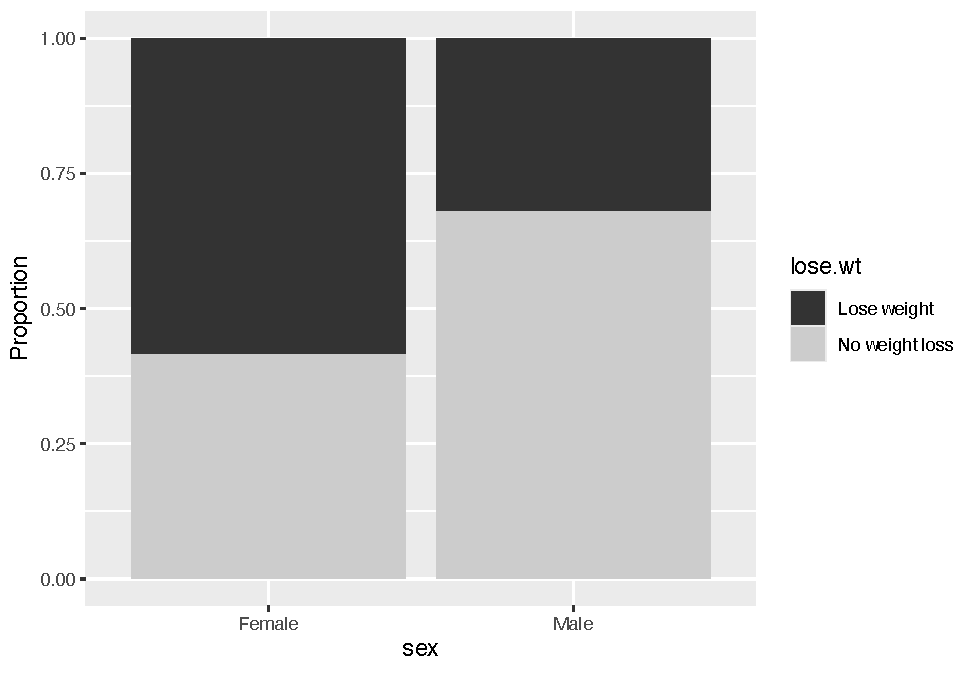
\includegraphics[width=0.6\linewidth]{bookdown-bysh_files/figure-latex/mosaicsexlose-1} 

}

\caption{Weight loss plans vs. Sex}\label{fig:mosaicsexlose}
\end{figure}

\begin{table}

\caption{\label{tab:table3chp6}Mean BMI percentile by sex and desire to lose weight.}
\centering
\begin{tabular}[t]{llllr}
\toprule
Sex & Weight loss status & mean BMI percentile & SD & n\\
\midrule
Female & No weight loss & 43.2 & 25.8 & 89\\
 & Lose weight & 72.4 & 23.0 & 125\\
Male & No weight loss & 58.8 & 28.2 & 157\\
 & Lose weight & 85.7 & 18.0 & 74\\
\bottomrule
\end{tabular}
\end{table}

Table \ref{tab:table3chp6} displays the mean BMI of those wanting and not wanting to lose weight for males and females. The mean BMI is greater for those trying to lose weight compared to those not trying to lose weight, regardless of sex. The size of the difference is remarkably similar for the two sexes.

If we consider including a BMI term in our model(s), the logit should be linearly related to BMI. We can investigate this assumption by constructing an empirical logit plot. In order to calculate empirical logits, we first divide our data by sex. Within each sex, we generate 10 groups of equal sizes, the first holding the bottom 10\% in BMI percentile for that sex, the second holding the next lowest 10\%, etc.. Within each group, we calculate the proporton, \(\hat{p}\) that reported wanting to lose weight, and then the empirical log odds, \(log(\frac{\hat{p}}{1-\hat{p}})\), that a young person in that group wants to lose weight.

\begin{figure}

{\centering 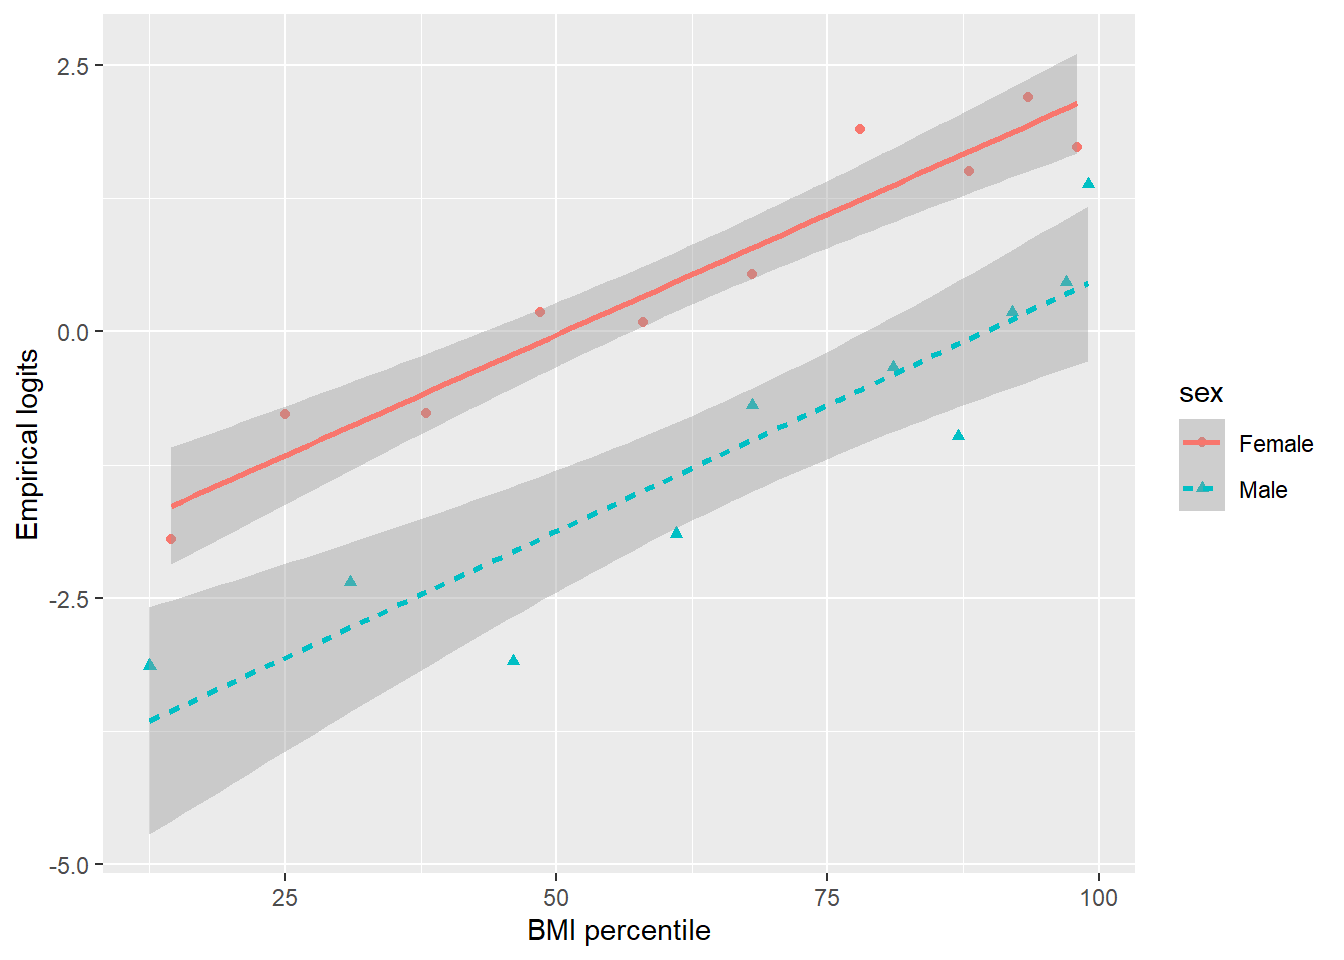
\includegraphics[width=0.6\linewidth]{bookdown-bysh_files/figure-latex/logitBMIsex-1} 

}

\caption{Empirical logits of trying to lose weight by BMI and Sex.}\label{fig:logitBMIsex}
\end{figure}

Figure \ref{fig:logitBMIsex} presents the empirical logits for the BMI intervals by sex. Both males and females exhibit an increasing linear trend on the logit scale indicating that increasing BMI is associated a greater desire to lose weight and that modeling log odds as a linear function of BMI is reasonable. The slope for the females appears to be similar to the slope for males, so we do not need to consider an interaction term between BMI and sex in the model.

\begin{figure}

{\centering 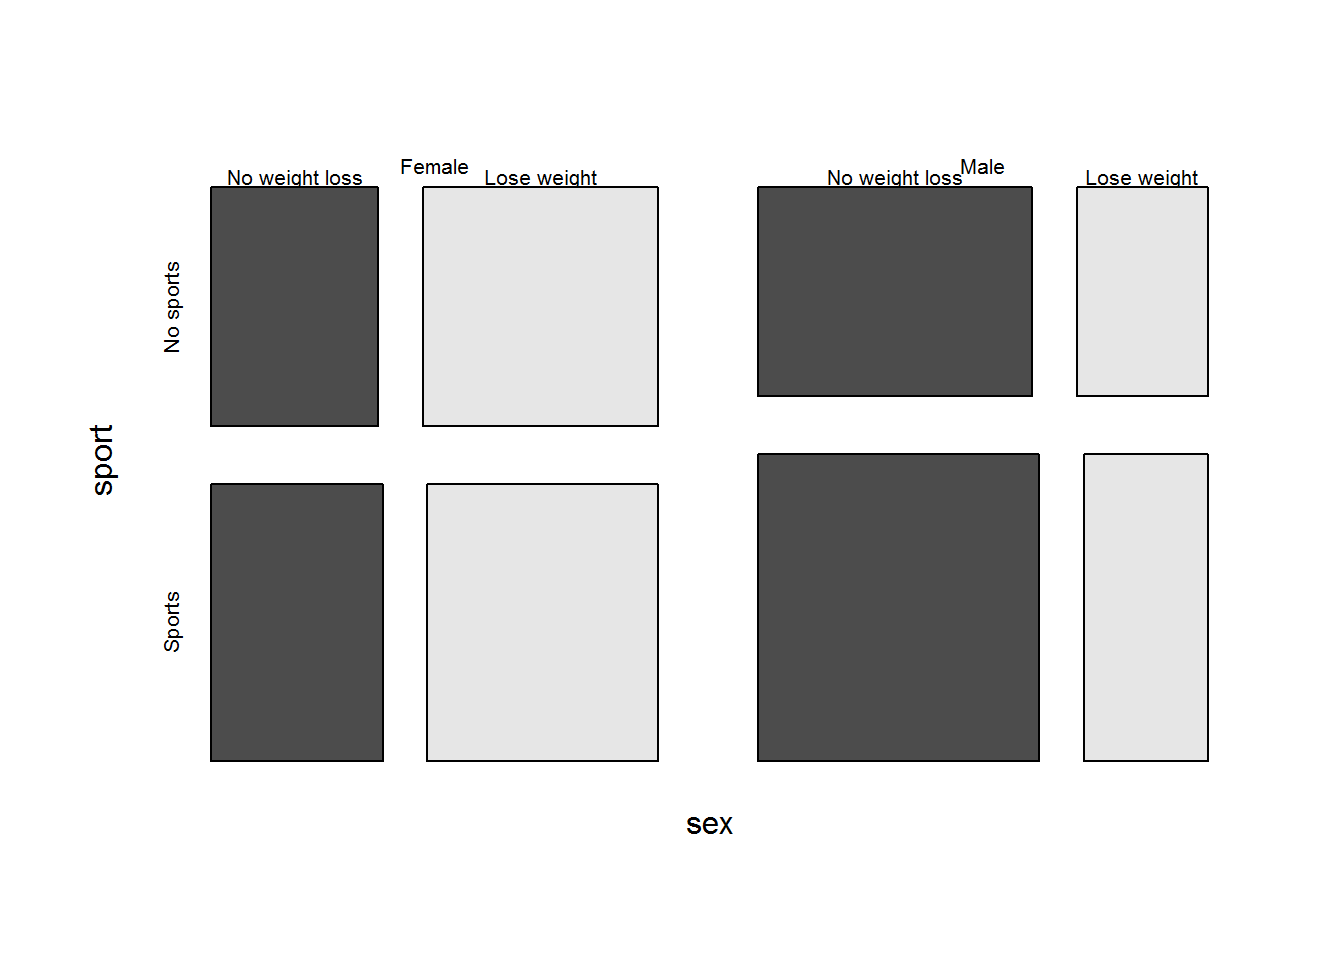
\includegraphics[width=0.6\linewidth]{bookdown-bysh_files/figure-latex/mosaicsexsports-1} 

}

\caption{Weight loss plans vs. sex and sports participation}\label{fig:mosaicsexsports}
\end{figure}

Out of those who play sports, 44\% want to lose weight whereas 46\% want to lose weight among those who do not play sports. Figure \ref{fig:mosaicsexsports} compares the proportion of respondents who want to lose weight by their sex and sport participation. The data suggest that sports participation is associated with the same or even a slightly lower desire to lose weight, contrary to what had originally been hypothesized. While the overall levels of those wanting to lose weight differ considerably between the sexes, the differences between those in and out of sports within sex appear to be very small. A term for sports participation or number of teams will be considered, but there is not compelling evidence that an interaction term will be needed.

It was posited that increased exposure to media, here measured as hours of TV daily, is associated with increased desire to lose weight, particularly for females. Overall, the percentage who want to lose weight ranges from 38\% of those watching 5 hours of TV per day to 55\% among those watching 2 hours daily. There is minimal variation in the proportion wanting to lose weight with both sexes combined. However, we are more interested in differences between the sexes (see Figure \ref{fig:mediaXsex}). We create empirical logits using the proportion of students trying to lose weight for each level of hours spent watching TV daily and look at the trends in the logits separately for males and females. From Figure \ref{fig:logitmediasex}, there does not appear to be a linear relationship for males or females.

\begin{figure}

{\centering 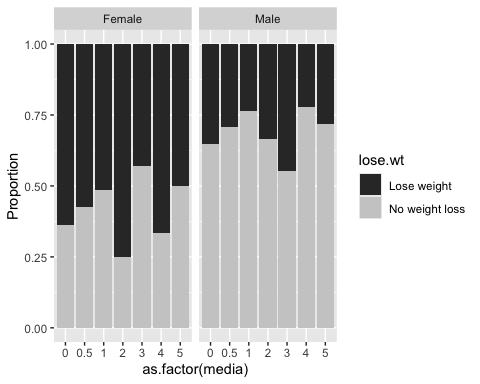
\includegraphics[width=0.6\linewidth]{bookdown-bysh_files/figure-latex/mediaXsex-1} 

}

\caption{Weight loss plans vs. daily hours of TV and sex.}\label{fig:mediaXsex}
\end{figure}

\begin{figure}

{\centering 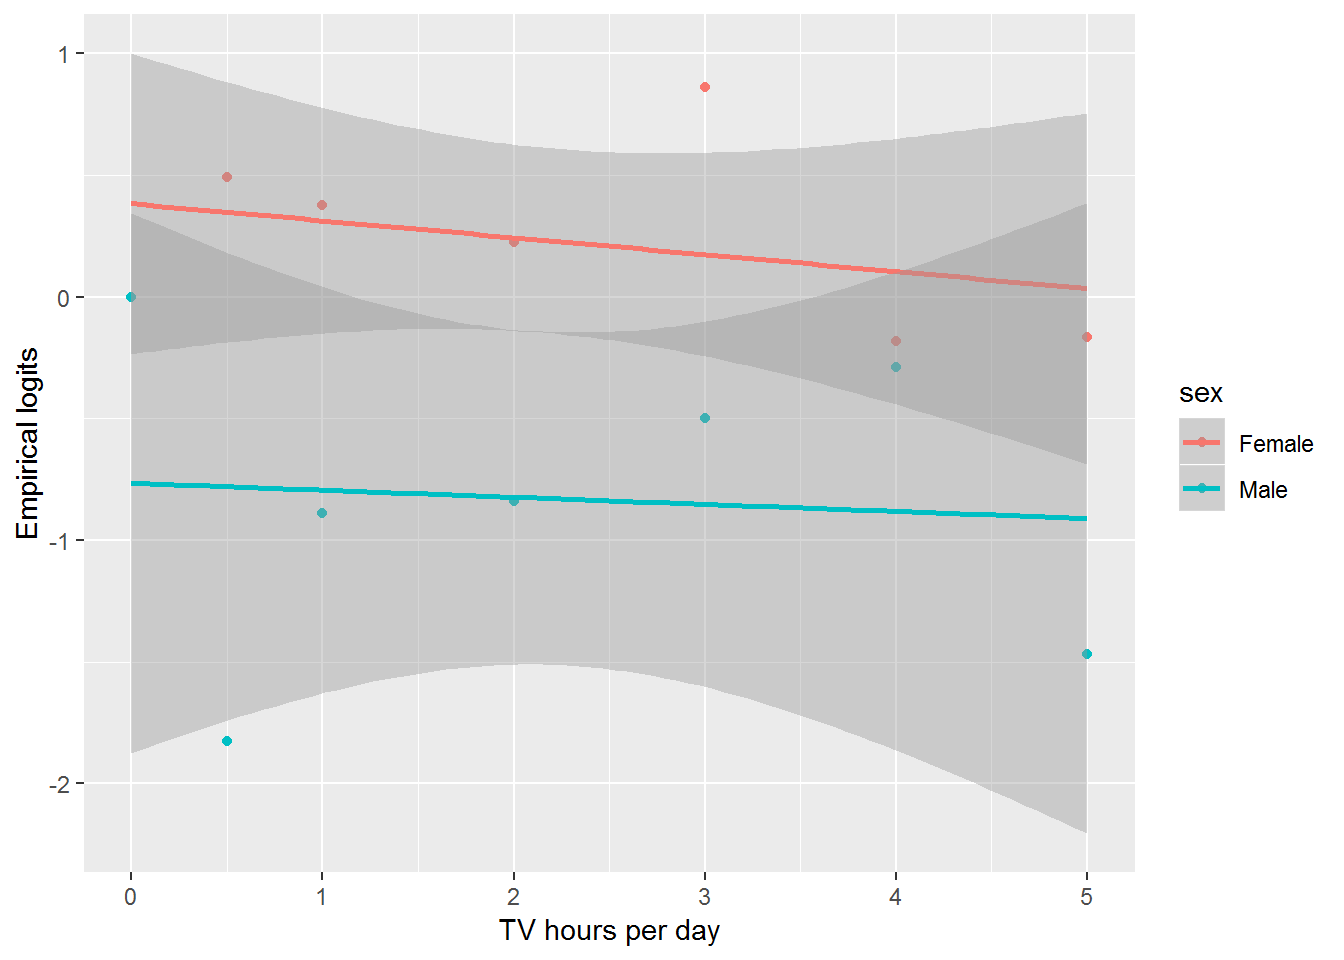
\includegraphics[width=0.6\linewidth]{bookdown-bysh_files/figure-latex/logitmediasex-1} 

}

\caption{Empirical logits for the odds of trying to lose weight by TV watching and sex.}\label{fig:logitmediasex}
\end{figure}

\hypertarget{initial-models-2}{%
\subsection{Initial Models}\label{initial-models-2}}

Our strategy for modeling is to use our questions of interest and what we have learned in the exploratory data analysis. For each model we interpret the coefficient of interest, look at the corresponding Wald test and, as a final step, compare the deviances for the different models we considered.

We first use a model where sex is our only predictor.

\begin{Shaded}
\begin{Highlighting}[]
\NormalTok{model1 <-}\StringTok{ }\KeywordTok{glm}\NormalTok{(lose.wt}\FloatTok{.01} \OperatorTok{~}\StringTok{ }\NormalTok{female, }\DataTypeTok{family =}\NormalTok{ binomial, }
              \DataTypeTok{data =}\NormalTok{ risk2009)}
\end{Highlighting}
\end{Shaded}

\begin{verbatim}
##             Estimate Std. Error z value  Pr(>|z|)
## (Intercept)  -0.7522     0.1410  -5.334 9.588e-08
## female        1.0919     0.1978   5.520 3.382e-08
\end{verbatim}

\begin{verbatim}
##  Residual deviance =  580.3  on  443 df
\end{verbatim}

Our estimated binomial regression model is:

\[\log\left(\frac{\hat{p}}{1-\hat{p}}\right)=-0.75+1.09 \textrm{female}\]
where \(\hat{p}\) is the estimated proportion of youth wanting to lose weight. We can interpret the coefficient on \texttt{female} by exponentiating \(e^{1.0919} = 2.98\) (95\% CI = \((2.03, 4.41)\)) indicating that the odds of a female trying to lose weight is nearly three times the odds of a male trying to lose weight (\(Z=5.520\), \(p=3.38e-08\)). We retain sex in the model and consider adding the BMI percentile:

\begin{Shaded}
\begin{Highlighting}[]
\NormalTok{model2 <-}\StringTok{ }\KeywordTok{glm}\NormalTok{(lose.wt}\FloatTok{.01} \OperatorTok{~}\StringTok{ }\NormalTok{female }\OperatorTok{+}\StringTok{ }\NormalTok{bmipct, }
              \DataTypeTok{family =}\NormalTok{ binomial, }\DataTypeTok{data =}\NormalTok{ risk2009)}
\end{Highlighting}
\end{Shaded}

\begin{verbatim}
##             Estimate Std. Error z value  Pr(>|z|)
## (Intercept) -4.25914    0.44927  -9.480 2.541e-21
## female       1.86067    0.25896   7.185 6.714e-13
## bmipct       0.04715    0.00524   8.997 2.313e-19
\end{verbatim}

\begin{verbatim}
##  Residual deviance =  463  on  442 df
\end{verbatim}

We see that there is statistically significant evidence (\(Z=8.997, p<.001\)) that BMI is positively associated with the odds of trying to lose weight, after controlling for sex. Clearly BMI percentile belongs in the model with sex.

Our estimated binomial regression model is:

\[\log\left(\frac{\hat{p}}{1-\hat{p}}\right)= -4.26+1.86\textrm{female}+0.047\textrm{bmipct}\]

To interpret the coefficient on \texttt{bmipct}, we will consider a 10 unit increase in \texttt{bmipct}. Because \(e^{10*0.047}=1.602\), then there is an estimated 60.2\% increase in the odds of wanting to lose weight for each additional 10 percentile points of BMI for members of the same sex. Just as we had done in other multiple regression models we need to interpret our coefficient \emph{given that the other variables remain constant}. An interaction term for BMI by sex was tested (not shown) and it was not significant (\(Z=-0.70\), \(p=0.485\)), so the effect of BMI does not differ by sex.

We next add \texttt{sport} to our model. Sports participation was considered for inclusion in the model in three ways: an indicator of sports participation (0 = no teams, 1 = one or more teams), treating the number of teams (0, 1, 2, or 3) as numeric, and treating the number of teams as a factor. The models below treat sports participation using an indicator variable, but all three models produced similar results.

\begin{Shaded}
\begin{Highlighting}[]
\NormalTok{model3 <-}\StringTok{ }\KeywordTok{glm}\NormalTok{(lose.wt}\FloatTok{.01} \OperatorTok{~}\StringTok{ }\NormalTok{female }\OperatorTok{+}\StringTok{ }\NormalTok{bmipct }\OperatorTok{+}\StringTok{ }\NormalTok{sport, }
              \DataTypeTok{family =}\NormalTok{ binomial, }\DataTypeTok{data =}\NormalTok{ risk2009)}
\end{Highlighting}
\end{Shaded}

\begin{verbatim}
##             Estimate Std. Error z value  Pr(>|z|)
## (Intercept) -4.17138   0.468463 -8.9044 5.367e-19
## female       1.84951   0.259514  7.1268 1.027e-12
## bmipct       0.04728   0.005251  9.0032 2.193e-19
## sportSports -0.14767   0.235101 -0.6281 5.299e-01
\end{verbatim}

\begin{verbatim}
##  Residual deviance =  462.6  on  441 df
\end{verbatim}

\begin{Shaded}
\begin{Highlighting}[]
\NormalTok{model3int <-}\StringTok{ }\KeywordTok{glm}\NormalTok{(lose.wt}\FloatTok{.01} \OperatorTok{~}\StringTok{ }\NormalTok{female }\OperatorTok{+}\StringTok{ }\NormalTok{bmipct }\OperatorTok{+}\StringTok{ }\NormalTok{sport }\OperatorTok{+}
\StringTok{              }\NormalTok{female}\OperatorTok{:}\NormalTok{sport }\OperatorTok{+}\StringTok{ }\NormalTok{bmipct}\OperatorTok{:}\NormalTok{sport, }
              \DataTypeTok{family =}\NormalTok{ binomial, }\DataTypeTok{data =}\NormalTok{ risk2009)}
\end{Highlighting}
\end{Shaded}

\begin{verbatim}
##                     Estimate Std. Error z value
## (Intercept)        -3.643635   0.604821  -6.024
## female              1.451017   0.378547   3.833
## bmipct              0.042530   0.007211   5.898
## sportSports        -1.187199   0.893057  -1.329
## female:sportSports  0.731516   0.523566   1.397
## bmipct:sportSports  0.009908   0.010463   0.947
##                     Pr(>|z|)
## (Intercept)        1.698e-09
## female             1.265e-04
## bmipct             3.684e-09
## sportSports        1.837e-01
## female:sportSports 1.624e-01
## bmipct:sportSports 3.436e-01
\end{verbatim}

\begin{verbatim}
##  Residual deviance =  460.5  on  439 df
\end{verbatim}

Sports teams were not significant in any of these models, nor were interaction terms (sex by sports and bmipct by sports). As a result, sports participation was no longer considered for inclusion in the model.

We last look at adding \texttt{media} to our model.

\begin{Shaded}
\begin{Highlighting}[]
\NormalTok{model4 <-}\StringTok{ }\KeywordTok{glm}\NormalTok{(lose.wt}\FloatTok{.01} \OperatorTok{~}\StringTok{ }\NormalTok{female }\OperatorTok{+}\StringTok{ }\NormalTok{bmipct }\OperatorTok{+}\StringTok{ }\NormalTok{media, }
              \DataTypeTok{family =}\NormalTok{ binomial, }\DataTypeTok{data =}\NormalTok{ risk2009)}
\end{Highlighting}
\end{Shaded}

\begin{verbatim}
##             Estimate Std. Error z value  Pr(>|z|)
## (Intercept) -4.08892   0.462947  -8.832 1.025e-18
## female       1.84776   0.259636   7.117 1.105e-12
## bmipct       0.04783   0.005287   9.046 1.485e-19
## media       -0.09938   0.072464  -1.371 1.702e-01
\end{verbatim}

\begin{verbatim}
##  Residual deviance =  461.1  on  441 df
\end{verbatim}

Media is not a statistically significant term (\(Z=-1.371\), \(p=0.170\)). However, because our interest centers on how media may affect attempts to lose weight and how its effect might be different for females and males, we fit a model with a media term and a sex by media interaction term (not shown). Neither term was statistically significant, so we have no support in our data that media exposure as measured by hours spent watching TV is associated with the odds a teen is trying to lose weight after accounting for sex and BMI.

\hypertarget{drop-in-deviance-tests}{%
\subsection{Drop-in-deviance Tests}\label{drop-in-deviance-tests}}

\begin{Shaded}
\begin{Highlighting}[]
\NormalTok{drop_in_dev <-}\StringTok{ }\KeywordTok{anova}\NormalTok{(model1, model2, model3, model4,}
                     \DataTypeTok{test=}\StringTok{"Chisq"}\NormalTok{)}
\end{Highlighting}
\end{Shaded}

\begin{verbatim}
  ResidDF ResidDev Deviance Df      pval
1     443    580.3       NA NA        NA
2     442    463.0 117.3301  1 2.431e-27
3     441    462.6   0.3947  1 5.298e-01
4     441    461.1   1.5007  0        NA
\end{verbatim}

\begin{verbatim}
       df   AIC
model1  2 584.3
model2  3 469.0
model3  4 470.6
model4  4 469.1
\end{verbatim}

Comparing models using differences in deviances requires that the models be \textbf{nested}, meaning each smaller model is a simplified version of the larger model. In our case, Models 1, 2, and 4 are nested, as are Models 1, 2, and 3, but Models 3 and 4 cannot be compared using a drop-in-deviance test.

There is a large drop-in-deviance adding BMI to the model with sex (Model 1 to Model 2, 117.3), which is clearly statistically significant when compared to a \(\chi^2\) distribution with 1 df. The drop-in-deviance for adding an indicator variable for sports to the model with sex and BMI is only 462.99 - 462.59 = 0.40. There is a difference of a single parameter, so the drop-in-deviance would be compared to a \(\chi^2\) distribution with 1 df. The resulting \(p\)-value is very large (.53) suggesting that adding an indicator for sports is not helpful once we've already accounted for BMI and sex. For comparing Models 3 and 4, one approach is to look at the AIC. In this case, the AIC is (barely) smaller for the model with media, providing evidence that the latter model is slightly preferable.

\hypertarget{model-discussion-and-summary}{%
\subsection{Model Discussion and Summary}\label{model-discussion-and-summary}}

We found that the odds of wanting to lose weight are considerably greater for females compared to males. In addition, respondents with greater BMI percentiles express a greater desire to lose weight for members of the same sex. Regardless of sex or BMI percentile, sports participation and TV watching are not associated with different odds for wanting to lose weight.

A limitation of this analysis is that we used complete cases in place of a method of imputing responses or modeling missingness. This reduced our sample from 500 to 445, and it may have introduced bias. For example, if respondents who watch a lot of TV were unwilling to reveal as much, and if they differed with respect to their desire to lose weight from those respondents who reported watching little TV, our inferences regarding the relationship between lots of TV and desire to lose weight may be biased.

Other limitations may result from definitions. Trying to lose weight is self-reported and may not correlate with any action undertaken to do so. The number of sports teams may not accurately reflect sports related pressures to lose weight. For example, elite athletes may focus on a single sport and be subject to greater pressures whereas athletes who casually participate in three sports may not feel any pressure to lose weight. Hours spent watching TV is not likely to encompass the totality of media exposure, particularly because exposure to celebrities occurs often online. Furthermore, this analysis does not explore in any detail maladaptions---inappropriate motivations for wanting to lose weight. For example, we did not focus our study on subsets of respondents with low BMI who are attempting to lose weight.

It would be instructive to use data science methodologies to explore the entire data set of 16,000 instead of sampling 500. However, the types of exploration and models used here could translate to the larger sample size.

Finally a limitation may be introduced as a result of the acknowledged variation in the administration of the YRBSS. States and local authorities are allowed to administer the survey as they see fit, which at times results in significant variation in sample selection and response.

\hypertarget{exercises-2}{%
\section{Exercises}\label{exercises-2}}

\hypertarget{conceptual-exercises}{%
\subsection{Conceptual Exercises}\label{conceptual-exercises}}

\begin{enumerate}
\def\labelenumi{\arabic{enumi}.}
\item
  List the explanatory and response variable(s) for each research question.

  \begin{enumerate}
  \def\labelenumii{\alph{enumii}.}
  \tightlist
  \item
    Are students with poor grades more likely to binge drink?
  \item
    What is the chance you are accepted into medical school given your GPA and MCAT scores?
  \item
    Is a single mom more likely to marry the baby's father if she has a boy?
  \item
    Are students participating in sports in college more or less likely to graduate?
  \item
    Is exposure to a particular chemical associated with a cancer diagnosis?
  \end{enumerate}
\item
  Interpret the odds ratios in the following abstract.

  \emph{Day Care Centers and Respiratory Health} \citep{Nafstad1999}

  \begin{itemize}
  \item
    \textbf{Objective}. To estimate the effects of the type of day care on respiratory health in preschool children.
  \item
    \textbf{Methods}. A population-based cross-sectional study of Oslo children born in 1992 was conducted at the end of 1996. A self-administered questionnaire inquired about day care arrangements, environmental conditions, and family characteristics (n = 3853; response rate, 79\%).
  \item
    \textbf{Results}. In a logistic regression controlling for confounding, children in day care centers had more often nightly cough (adjusted odds ratio, 1.89; 95\% confidence interval 1.34-2.67), and blocked or runny nose without common cold (1.55; 1.07-1.61) during the past 12 months compared with children in home care\ldots{}
  \end{itemize}
\item
  Construct a table and calculate the corresponding odds and odds ratios. Comment on the reported and calculated results in this \emph{New York Times} article from \citet{Kolata2009}.

  \begin{itemize}
  \item
    In November, the Centers for Disease Control and Prevention published a paper reporting that babies conceived with IVF, or with a technique in which sperm are injected directly into eggs, have a slightly increased risk of several birth defects, including a hole between the two chambers of the heart, a cleft lip or palate, an improperly developed esophagus and a malformed rectum. The study involved 9,584 babies with birth defects and 4,792 babies without. Among the mothers of babies without birth defects, 1.1 percent had used IVF or related methods, compared with 2.4 percent of mothers of babies with birth defects.
  \item
    The findings are considered preliminary, and researchers say they believe IVF does not carry excessive risks. There is a 3 percent chance that any given baby will have a birth defect.
  \end{itemize}
\item
  In a small pilot study, researchers compared two groups of 3 turbine wheels each under low humidity and two groups of 3 turbine wheels each under high humidity conditions to determine if humidity is related to the number of fissures that occur. If \(Y\) = number of turbine wheels that develop fissures, then assume that \(Y \sim \textrm{Binomial}(n=3, p=p_L)\) under low humidity, and \(Y \sim \textrm{Binomial}(n=3, p=p_H)\) under high humidity, where \(f(y;p)=\binom{n}{y} p^y (1-p)^{n-y}\). Write out the log-likelihood function \(\textrm{logL}(p_L, p_H)\), using the data in Table \ref{tab:fissurechp6} and simplifying where possible.
\end{enumerate}

\begin{table}

\caption{\label{tab:fissurechp6}Data for Conceptual Exercise 4}
\centering
\begin{tabular}[t]{>{\raggedright\arraybackslash}p{2cm}llll}
\toprule
Turbine group & 1 & 2 & 3 & 4\\
\midrule
Humidity & Low & Low & High & High\\
n = number of turbine wheels & 3 & 3 & 3 & 3\\
y = number of fissures & 1 & 2 & 1 & 0\\
\bottomrule
\end{tabular}
\end{table}

\hypertarget{guided-exercises-1}{%
\subsection{Guided Exercises}\label{guided-exercises-1}}

\begin{enumerate}
\def\labelenumi{\arabic{enumi}.}
\item
  \textbf{Soccer goals on target.} Data comes from an article in \emph{Psychological Science} \citep{Roskes2011}. The authors report on the success rate of penalty kicks that were on-target, so that either the keeper saved the shot or the shot scored, for FIFA World Cup shootouts between 1982 and 2010. They found that 18 out of 20 shots were scored when the goalkeeper's team was behind, 71 out of 90 shots were scored when the game was tied, and 55 out of 75 shots were scored with the goalkeeper's team ahead.

  \begin{enumerate}
  \def\labelenumii{\alph{enumii}.}
  \item
    Calculate the odds of a successful penalty kick for games in which the goalkeeper's team was behind, tied, or ahead. Then, construct empirical odds ratios for successful penalty kicks for (a) behind versus tied, and (b) tied versus ahead.
  \item
    Fit a model with the categorical predictor c(``behind'',``tied'',``ahead'') and interpret the exponentiated coefficients. How do they compare to the empirical odds ratios you calculated?
  \end{enumerate}
\item
  \textbf{Medical School Admissions.} The data for Medical School Admissions is in \texttt{MedGPA.csv}, taken from undergraduates from a small liberal arts school over several years. We are interested in student attributes that are associated with higher acceptance rates.

  \begin{itemize}
  \tightlist
  \item
    \texttt{Accept} = accepted (A) into medical school or denied (D)
  \item
    \texttt{Acceptance} = accepted (1) into medical school or denied (0)
  \item
    \texttt{Sex} = male (M) or female (F)
  \item
    \texttt{BCPM} = GPA in natural sciences and mathematics
  \item
    \texttt{GPA} = overall GPA
  \item
    \texttt{VR} = verbal reasoning subscale score of the MCAT
  \item
    \texttt{PS} = physical sciences subscale score of the MCAT
  \item
    \texttt{WS} = writing samples subscale score of the MCAT
  \item
    \texttt{BS} = biological sciences subscale score of the MCAT
  \item
    \texttt{MCAT} = MCAT total score
  \item
    \texttt{Apps} = number of schools applied to
  \end{itemize}

  Be sure to interpret model coefficients and associated tests of significance or confidence intervals when answering the following questions:

  \begin{enumerate}
  \def\labelenumii{\alph{enumii}.}
  \tightlist
  \item
    Compare the relative effects of improving your MCAT score versus improving your GPA on your odds of being accepted to medical school.
  \item
    After controlling for MCAT and GPA, is the number of applications related to odds of getting into medical school?
  \item
    Is one MCAT subscale more important than the others?
  \item
    Is there any evidence that the effect of MCAT score or GPA differs for males and females?
  \end{enumerate}
\item
  \textbf{Moths.} An article in the \emph{Journal of Animal Ecology} by \citet{Bishop1972} investigated whether moths provide evidence of ``survival of the fittest'' with their camouflage traits. Researchers glued equal numbers of light and dark morph moths in lifelike positions on tree trunks at 7 locations from 0 to 51.2 km from Liverpool. They then recorded the numbers of moths removed after 24 hours, presumably by predators. The hypothesis was that, since tree trunks near Liverpool were blackened by pollution, light morph moths would be more likely to be removed near Liverpool.

  Data \citep{Ramsey2002} can be found in \texttt{moth.csv} and contains the variables below. In addition, R code at the end of the problem can be used to input the data and create additional useful variables.

  \begin{itemize}
  \tightlist
  \item
    \texttt{MOPRH} = light or dark
  \item
    \texttt{DISTANCE} = kilometers from Liverpool
  \item
    \texttt{PLACED} = number of moths of a specific morph glued to trees at that location
  \item
    \texttt{REMOVED} = number of moths of a specific morph removed after 24 hours
  \end{itemize}

  \begin{enumerate}
  \def\labelenumii{\alph{enumii}.}
  \tightlist
  \item
    What are logits in this study?
  \item
    Create an empirical logit plot of logits vs.~distance by morph. What can we conclude from this plot?
  \item
    Create a model with \texttt{DISTANCE} and \texttt{dark}. Interpret all the coefficients.
  \item
    Create a model with \texttt{DISTANCE}, \texttt{dark}, and the interaction between both variables. Interpret all the coefficients.
  \item
    Interpret a drop-in-deviance test and a Wald test to test the significance of the interaction term in (d).
  \item
    Test the goodness of fit for the interaction model. What can we conclude about this model?
  \item
    Is there evidence of overdispersion in the interaction model? What factors might lead to overdispersion in this case? Regardless of your answer, repeat (d) adjusting for overdispersion.
  \item
    Compare confidence intervals for coefficients in your models from (g) and (d).
  \item
    What happens if we expand the data set to contain one row per moth (968 rows)? Now we can run a logistic binary regression model. How does the logistic binary regression model compare to the binomial regression model? What are similarities and differences? Would there be any reason to run a logistic binomial regression rather than a logistic binary regression in a case like this? Some starter code can be found below the input code.
  \end{enumerate}
\end{enumerate}

\begin{Shaded}
\begin{Highlighting}[]
\NormalTok{moth <-}\StringTok{ }\KeywordTok{read_csv}\NormalTok{(}\StringTok{"data/moth.csv"}\NormalTok{)}
\NormalTok{moth <-}\StringTok{ }\KeywordTok{mutate}\NormalTok{(moth, }
               \DataTypeTok{notremoved =}\NormalTok{ PLACED }\OperatorTok{-}\StringTok{ }\NormalTok{REMOVED, }
               \DataTypeTok{logit1 =} \KeywordTok{log}\NormalTok{(REMOVED }\OperatorTok{/}\StringTok{ }\NormalTok{notremoved),}
               \DataTypeTok{prop1 =}\NormalTok{ REMOVED }\OperatorTok{/}\StringTok{ }\NormalTok{PLACED, }
               \DataTypeTok{dark =} \KeywordTok{ifelse}\NormalTok{(MORPH}\OperatorTok{==}\StringTok{"dark"}\NormalTok{,}\DecValTok{1}\NormalTok{,}\DecValTok{0}\NormalTok{) )}
\end{Highlighting}
\end{Shaded}

\begin{Shaded}
\begin{Highlighting}[]
\NormalTok{mtemp1 =}\StringTok{ }\KeywordTok{rep}\NormalTok{(moth}\OperatorTok{$}\NormalTok{dark[}\DecValTok{1}\NormalTok{],moth}\OperatorTok{$}\NormalTok{REMOVED[}\DecValTok{1}\NormalTok{])}
\NormalTok{dtemp1 =}\StringTok{ }\KeywordTok{rep}\NormalTok{(moth}\OperatorTok{$}\NormalTok{DISTANCE[}\DecValTok{1}\NormalTok{],moth}\OperatorTok{$}\NormalTok{REMOVED[}\DecValTok{1}\NormalTok{])}
\NormalTok{rtemp1 =}\StringTok{ }\KeywordTok{rep}\NormalTok{(}\DecValTok{1}\NormalTok{,moth}\OperatorTok{$}\NormalTok{REMOVED[}\DecValTok{1}\NormalTok{])}
\NormalTok{mtemp1 =}\StringTok{ }\KeywordTok{c}\NormalTok{(mtemp1,}\KeywordTok{rep}\NormalTok{(moth}\OperatorTok{$}\NormalTok{dark[}\DecValTok{1}\NormalTok{],}
\NormalTok{                      moth}\OperatorTok{$}\NormalTok{PLACED[}\DecValTok{1}\NormalTok{]}\OperatorTok{-}\NormalTok{moth}\OperatorTok{$}\NormalTok{REMOVED[}\DecValTok{1}\NormalTok{]))}
\NormalTok{dtemp1 =}\StringTok{ }\KeywordTok{c}\NormalTok{(dtemp1,}\KeywordTok{rep}\NormalTok{(moth}\OperatorTok{$}\NormalTok{DISTANCE[}\DecValTok{1}\NormalTok{],}
\NormalTok{                      moth}\OperatorTok{$}\NormalTok{PLACED[}\DecValTok{1}\NormalTok{]}\OperatorTok{-}\NormalTok{moth}\OperatorTok{$}\NormalTok{REMOVED[}\DecValTok{1}\NormalTok{]))}
\NormalTok{rtemp1 =}\StringTok{ }\KeywordTok{c}\NormalTok{(rtemp1,}\KeywordTok{rep}\NormalTok{(}\DecValTok{0}\NormalTok{,moth}\OperatorTok{$}\NormalTok{PLACED[}\DecValTok{1}\NormalTok{]}\OperatorTok{-}\NormalTok{moth}\OperatorTok{$}\NormalTok{REMOVED[}\DecValTok{1}\NormalTok{]))}
\ControlFlowTok{for}\NormalTok{(i }\ControlFlowTok{in} \DecValTok{2}\OperatorTok{:}\DecValTok{14}\NormalTok{)  \{}
\NormalTok{  mtemp1 =}\StringTok{ }\KeywordTok{c}\NormalTok{(mtemp1,}\KeywordTok{rep}\NormalTok{(moth}\OperatorTok{$}\NormalTok{dark[i],moth}\OperatorTok{$}\NormalTok{REMOVED[i]))}
\NormalTok{  dtemp1 =}\StringTok{ }\KeywordTok{c}\NormalTok{(dtemp1,}\KeywordTok{rep}\NormalTok{(moth}\OperatorTok{$}\NormalTok{DISTANCE[i],moth}\OperatorTok{$}\NormalTok{REMOVED[i]))}
\NormalTok{  rtemp1 =}\StringTok{ }\KeywordTok{c}\NormalTok{(rtemp1,}\KeywordTok{rep}\NormalTok{(}\DecValTok{1}\NormalTok{,moth}\OperatorTok{$}\NormalTok{REMOVED[i]))}
\NormalTok{  mtemp1 =}\StringTok{ }\KeywordTok{c}\NormalTok{(mtemp1,}\KeywordTok{rep}\NormalTok{(moth}\OperatorTok{$}\NormalTok{dark[i],}
\NormalTok{                        moth}\OperatorTok{$}\NormalTok{PLACED[i]}\OperatorTok{-}\NormalTok{moth}\OperatorTok{$}\NormalTok{REMOVED[i]))}
\NormalTok{  dtemp1 =}\StringTok{ }\KeywordTok{c}\NormalTok{(dtemp1,}\KeywordTok{rep}\NormalTok{(moth}\OperatorTok{$}\NormalTok{DISTANCE[i],}
\NormalTok{                        moth}\OperatorTok{$}\NormalTok{PLACED[i]}\OperatorTok{-}\NormalTok{moth}\OperatorTok{$}\NormalTok{REMOVED[i]))}
\NormalTok{  rtemp1 =}\StringTok{ }\KeywordTok{c}\NormalTok{(rtemp1,}\KeywordTok{rep}\NormalTok{(}\DecValTok{0}\NormalTok{,moth}\OperatorTok{$}\NormalTok{PLACED[i]}\OperatorTok{-}\NormalTok{moth}\OperatorTok{$}\NormalTok{REMOVED[i]))  \}}
\NormalTok{newdata =}\StringTok{ }\KeywordTok{data.frame}\NormalTok{(}\DataTypeTok{removed=}\NormalTok{rtemp1,}\DataTypeTok{dark=}\NormalTok{mtemp1,}\DataTypeTok{dist=}\NormalTok{dtemp1)}
\NormalTok{newdata[}\DecValTok{1}\OperatorTok{:}\DecValTok{25}\NormalTok{,]}
\KeywordTok{cdplot}\NormalTok{(}\KeywordTok{as.factor}\NormalTok{(rtemp1)}\OperatorTok{~}\NormalTok{dtemp1)}
\end{Highlighting}
\end{Shaded}

\begin{enumerate}
\def\labelenumi{\arabic{enumi}.}
\setcounter{enumi}{3}
\item
  \textbf{Birdkeeping and Lung Cancer: A Retrospective Observational Study} A 1972-1981 health survey in The Hague, Netherlands, discovered an association between keeping pet birds and increased risk of lung cancer. To investigate birdkeeping as a risk factor, researchers conducted a case-control study of patients in 1985 at four hospitals in The Hague. They identified 49 cases of lung cancer among patients who were registered with a general practice, who were age 65 or younger, and who had resided in the city since 1965. Each patient (case) with cancer was matched with two control subjects (without cancer) by age and sex. Further details can be found in \citet{Holst1988}.

  Age, sex, and smoking history are all known to be associated with lung cancer incidence. Thus, researchers wished to determine after age, sex, socioeconomic status, and smoking have been controlled for, is an additional risk associated with birdkeeping? The data \citep{Ramsey2002} is found in \texttt{birdkeeping.csv}, and the variables are listed below. In addition, R code at the end of the problem can be used to input the data and create additional useful variables.

  \begin{itemize}
  \tightlist
  \item
    \texttt{female} = sex (1 = Female, 0 = Male)
  \item
    \texttt{age} = age, in years
  \item
    \texttt{highstatus} = socioeconomic status (1 = High, 0 = Low), determined by the occupation of the household's primary wage earner
  \item
    \texttt{yrsmoke} = years of smoking prior to diagnosis or examination
  \item
    \texttt{cigsday} = average rate of smoking, in cigarettes per day
  \item
    \texttt{bird} = indicator of birdkeeping (1 = Yes, 0 = No), determined by whether or not there were caged birds in the home for more than 6 consecutive months from 5 to 14 years before diagnosis (cases) or examination (controls)
  \item
    \texttt{cancer} = indicator of lung cancer diagnosis (1 = Cancer, 0 = No Cancer)
  \end{itemize}

  \begin{enumerate}
  \def\labelenumii{\alph{enumii}.}
  \tightlist
  \item
    Perform an exploratory data analysis to see how each explanatory variable is related to the response (\texttt{cancer}). Summarize each relationship in one sentence.
  \end{enumerate}

  \begin{itemize}
  \item
    For quantitative explanatory variables (\texttt{age}, \texttt{yrsmoke}, \texttt{cigsday}), produce a cdplot, a boxplot, and summary statistics by cancer diagnosis.
  \item
    For categorical explanatory variables (\texttt{female} or \texttt{sex}, \texttt{highstatus} or \texttt{socioecon\_status}, \texttt{bird} or \texttt{keep\_bird}), produce a segmented bar chart and an appropriate table of proportions showing the relationship with cancer diagnosis.
  \end{itemize}

  \begin{enumerate}
  \def\labelenumii{\alph{enumii}.}
  \setcounter{enumii}{1}
  \item
    In (a), you should have found no relationship between whether or not a patient develops lung cancer and either their age or sex. Why might this be? What implications will this have on your modeling?
  \item
    Based on a two-way table with keeping birds and developing lung cancer from (a), find an unadjusted odds ratio comparing birdkeepers to non-birdkeepers and interpret this odds ratio in context. (Note: an \emph{unadjusted} odds ratio is found by \emph{not} controlling for any other variables.) Also, find an analogous relative risk and interpret it in context as well.
  \item
    Are the elogits reasonably linear relating number of years smoked to the estimated log odds of developing lung cancer? Demonstrate with an appropriate plot.
  \item
    Does there appear to be an interaction between number of years smoked and whether the subject keeps a bird? Demonstrate with an interaction plot and a coded scatterplot with empirical logits on the y-axis.
  \end{enumerate}

  Before answering the next questions, fit logistic regression models in R with \texttt{cancer} as the response and the following sets of explanatory variables:

  \begin{itemize}
  \tightlist
  \item
    \texttt{model1} = \texttt{age}, \texttt{yrsmoke}, \texttt{cigsday}, \texttt{female}, \texttt{highstatus}, \texttt{bird}
  \item
    \texttt{model2} = \texttt{yrsmoke}, \texttt{cigsday}, \texttt{highstatus}, \texttt{bird}
  \item
    \texttt{model4} = \texttt{yrsmoke}, \texttt{bird}
  \item
    \texttt{model5} = the complete second order version of \texttt{model4} (add squared terms and an interaction)
  \item
    \texttt{model6} = \texttt{yrsmoke}, \texttt{bird}, \texttt{yrsmoke:bird}
  \end{itemize}

  \begin{enumerate}
  \def\labelenumii{\alph{enumii}.}
  \setcounter{enumii}{5}
  \item
    Is there evidence that we can remove \texttt{age} and \texttt{female} from our model? Perform an appropriate test comparing \texttt{model1} to \texttt{model2}; give a test statistic and p-value, and state a conclusion in context.
  \item
    Is there evidence that the complete second order version of \texttt{model4} improves its performance? Perform an appropriate test comparing \texttt{model4} to \texttt{model5}; give a test statistic and p-value, and state a conclusion in context.
  \item
    Carefully interpret each of the four model coefficients in \texttt{model6} in context.
  \item
    If you replaced \texttt{yrsmoke} everywhere it appears in \texttt{model6} with a mean-centered version of \texttt{yrsmoke}, tell what would change among these elements: the 4 coefficients, the 4 p-values for coefficients, and the residual deviance.
  \item
    \texttt{model4} is a potential final model based on this set of explanatory variables. Find and carefully interpret 95\% confidence intervals based on profile likelihoods for the coefficients of \texttt{yrsmoke} and \texttt{bird}.
  \item
    How does the adjusted odds ratio for birdkeeping from \texttt{model4} compare with the unadjusted odds ratio you found in (c)? Is birdkeeping associated with a significant increase in the odds of developing lung cancer, even after adjusting for other factors?
  \item
    Use the categorical variable \texttt{years\_factor} based on \texttt{yrsmoke} and replace \texttt{yrsmoke} in \texttt{model4} with your new variable to create \texttt{model4a}. First, interpret the coefficient for \texttt{years\_factorOver\ 25\ years} in context. Then tell if you prefer \texttt{model4} with years smoked as a numeric predictor or \texttt{model4a} with years smoked as a categorical predictor, and explain your reasoning.
  \item
    Discuss the scope of inference in this study. Can we generalize our findings beyond the subjects in this study? Can we conclude that birdkeeping causes increased odds of developing lung cancer? Do you have other concerns with this study design or the analysis you carried out?
  \item
    Read the article that appeared in the \emph{British Medical Journal}. What similarities and differences do you see between their analyses and yours? What are a couple of things you learned from the article that weren't apparent in the short summary at the beginning of the assignment.
  \end{enumerate}
\end{enumerate}

\begin{Shaded}
\begin{Highlighting}[]
\NormalTok{birds <-}\StringTok{ }\KeywordTok{read_csv}\NormalTok{(}\StringTok{"data/birdkeeping.csv"}\NormalTok{) }\OperatorTok
\StringTok{  }\KeywordTok{mutate}\NormalTok{(}\DataTypeTok{sex =} \KeywordTok{ifelse}\NormalTok{(female }\OperatorTok{==}\StringTok{ }\DecValTok{1}\NormalTok{, }\StringTok{"Female"}\NormalTok{, }\StringTok{"Male"}\NormalTok{),}
         \DataTypeTok{socioecon_status =} \KeywordTok{ifelse}\NormalTok{(highstatus }\OperatorTok{==}\StringTok{ }\DecValTok{1}\NormalTok{, }
                                   \StringTok{"High"}\NormalTok{, }\StringTok{"Low"}\NormalTok{),}
         \DataTypeTok{keep_bird =} \KeywordTok{ifelse}\NormalTok{(bird }\OperatorTok{==}\StringTok{ }\DecValTok{1}\NormalTok{, }\StringTok{"Keep Bird"}\NormalTok{, }\StringTok{"No Bird"}\NormalTok{),}
         \DataTypeTok{lung_cancer =} \KeywordTok{ifelse}\NormalTok{(cancer }\OperatorTok{==}\StringTok{ }\DecValTok{1}\NormalTok{, }\StringTok{"Cancer"}\NormalTok{, }
                              \StringTok{"No Cancer"}\NormalTok{)) }\OperatorTok
\StringTok{  }\KeywordTok{mutate}\NormalTok{(}\DataTypeTok{years_factor =} \KeywordTok{cut}\NormalTok{(yrsmoke, }
                            \DataTypeTok{breaks =} \KeywordTok{c}\NormalTok{(}\OperatorTok{-}\OtherTok{Inf}\NormalTok{, }\DecValTok{0}\NormalTok{, }\DecValTok{25}\NormalTok{, }\OtherTok{Inf}\NormalTok{),}
            \DataTypeTok{labels =} \KeywordTok{c}\NormalTok{(}\StringTok{"No smoking"}\NormalTok{, }\StringTok{"1-25 years"}\NormalTok{, }
                       \StringTok{"Over 25 years"}\NormalTok{)))}
\end{Highlighting}
\end{Shaded}

\begin{enumerate}
\def\labelenumi{\arabic{enumi}.}
\setcounter{enumi}{4}
\item
  \textbf{2016 Election.} An \href{https://www.causeweb.org/usproc/usclap/2018/spring/winners}{award-winning} student project \citep{Renier2018} examined driving forces behind Donald Trump's surprising victory in the 2016 Presidential Election, using data from nearly 40,000 voters collected as part of the 2016 Cooperative Congressional Election Survey (CCES). The student researchers investigated two theories: (1) Trump was seen as the candidate of change for voters experiencing economic hardship, and (2) Trump exploited voter fears about immigrants and minorities.

  The dataset \texttt{electiondata.csv} has individual level data on voters in the 2016 Presidential election, collected from the CCES and subsequently tidied. We will focus on the following variables:

  \begin{itemize}
  \tightlist
  \item
    \texttt{Vote} = 1 if Trump; 0 if another candidate
  \item
    \texttt{zfaminc} = family income expressed as a z-score (number of standard deviations above or below the mean)
  \item
    \texttt{zmedinc} = state median income expressed as a z-score
  \item
    \texttt{EconWorse} = 1 if the voter believed the economy had gotten worse in the past 4 years; 0 otherwise
  \item
    \texttt{EducStatus} = 1 if the voter had at least a bachelor's degree; 0 otherwise
  \item
    \texttt{republican} = 1 if the voter identified as Republican; 0 otherwise
  \item
    \texttt{Noimmigrants} = 1 if the voter supported at least 1 of 2 anti-immigrant policy statements; 0 if neither
  \item
    \texttt{propforeign} = proportion foreign born in the state
  \item
    \texttt{evangelical} = 1 if \texttt{pew\_bornagain} is 2; otherwise 0
  \end{itemize}

  The questions below address Theory 1 (Economic Model). We want to see if there is significant evidence that voting for Trump was associated with family income level and/or with a belief that the economy became worse during the Obama Administration.

  \begin{enumerate}
  \def\labelenumii{\alph{enumii}.}
  \tightlist
  \item
    Create a plot showing the relationship between whether a voter voted for Trump and their opinion about the status of the economy. What do you find?
  \item
    Repeat (a) separately for Republicans and non-Republicans. Again describe what you find.
  \item
    Create a plot with one observation per state showing the relationship between a state's median income and the log odds of a resident of that state voting for Trump. What can you conclude from this plot?
  \end{enumerate}

  Answer (d)-(f) based on \texttt{model1a} below:

  \begin{enumerate}
  \def\labelenumii{\alph{enumii}.}
  \setcounter{enumii}{3}
  \tightlist
  \item
    Interpret the coefficient for \texttt{zmedinc} in context.
  \item
    Interpret the coefficient for \texttt{republican} in context.
  \item
    Interpret the coefficient for \texttt{EconWorse:republican} in context. What does this allow us to conclude about Theory 1?\\
  \item
    Repeat the above process for Theory 2 (Immigration Model). That is, produce meaningful exploratory plots, fit a model to the data with special emphasis on \texttt{Noimmigrants}, interpret meaningful coefficients, and state what can be concluded about Theory 2.
  \item
    Is there any concern about the independence assumption in these models? We will return to this question in later chapters.
  \end{enumerate}
\end{enumerate}

\begin{Shaded}
\begin{Highlighting}[]
\NormalTok{model1a <-}\StringTok{ }\KeywordTok{glm}\NormalTok{(Vote01 }\OperatorTok{~}\StringTok{ }\NormalTok{zfaminc }\OperatorTok{+}\StringTok{ }\NormalTok{zmedinc }\OperatorTok{+}\StringTok{ }\NormalTok{EconWorse }\OperatorTok{+}
\StringTok{    }\NormalTok{EducStatus }\OperatorTok{+}\StringTok{ }\NormalTok{republican }\OperatorTok{+}\StringTok{ }\NormalTok{EducStatus}\OperatorTok{:}\NormalTok{republican }\OperatorTok{+}
\StringTok{    }\NormalTok{EconWorse}\OperatorTok{:}\NormalTok{zfaminc }\OperatorTok{+}\StringTok{ }\NormalTok{EconWorse}\OperatorTok{:}\NormalTok{republican, }
    \DataTypeTok{family =}\NormalTok{ binomial, }\DataTypeTok{data =}\NormalTok{ electiondata)}
\KeywordTok{summary}\NormalTok{(model1a)}
\end{Highlighting}
\end{Shaded}

\hypertarget{open-ended-exercises-1}{%
\subsection{Open-ended Exercises}\label{open-ended-exercises-1}}

\begin{enumerate}
\def\labelenumi{\arabic{enumi}.}
\item
  \textbf{2008 Presidential Voting in Minnesota counties.} Data in \texttt{mn08.csv} contains results from the 2008 US Presidential election by county in Minnesota, focusing on the two primary candidates (Democrat Barack Obama and Republican John McCain). You can consider the response to be either the percent of Obama votes in a county (binomial) or whether or not Obama had more votes than McCain (binary). Then build a model for your response using county-level predictors listed below. Interpret the results of your model.

  \begin{itemize}
  \tightlist
  \item
    \texttt{County} = county name
  \item
    \texttt{Obama} = total votes for Obama
  \item
    \texttt{McCain} = total votes for McCain
  \item
    \texttt{pct\_Obama} = percent of votes for Obama
  \item
    \texttt{pct\_rural} = percent of county who live in a rural setting
  \item
    \texttt{medHHinc} = median household income
  \item
    \texttt{unemp\_rate} = unemployment rate
  \item
    \texttt{pct\_poverty} = percent living below the poverty line
  \item
    \texttt{medAge2007} = median age in 2007
  \item
    \texttt{medAge2000} = median age in 2000
  \item
    \texttt{Gini\_Index} = measure of income disparity in a county
  \item
    \texttt{pct\_native} = percent of native born residents
  \end{itemize}
\item
  \textbf{Crime on Campus.} The data set \texttt{c\_data2.csv} contains statistics on violent crimes and property crimes for a sample of 81 US colleges and universities. Characterize rates of violent crimes as a proportion of total crimes reported (i.e., \texttt{num\_viol} / \texttt{total\_crime}) -- do they differ based on type of institution, size of institution, or region of the country?

  \begin{itemize}
  \tightlist
  \item
    \texttt{Enrollment} = number of students enrolled
  \item
    \texttt{type} = university (U) or college (C)
  \item
    \texttt{num\_viol} = number of violent crimes reported
  \item
    \texttt{num\_prop} = number of property crimes reported
  \item
    \texttt{viol\_rate\_10000} = violent crime rate per 10000 students enrolled
  \item
    \texttt{prop\_rate\_10000} = property crime rate per 10000 students enrolled
  \item
    \texttt{total\_crime} = total crimes reported (property and violent)
  \item
    \texttt{region} = region of the country
  \end{itemize}
\item
  \textbf{NBA Data.} Data in \texttt{NBA1718team.csv} \citep{rossotti} looks at factors that are associated with a pro basketball team's winning percentage in the 2017-18 season. After a thorough exploratory data analyses, create the best model you can to predict a team's winning percentage; be careful of collinearity between the covariates. Based on your EDA and modeling, describe the factors that seem to explain a team's success.

  \begin{itemize}
  \tightlist
  \item
    \texttt{win\_pct} = Percentage of Wins,
  \item
    \texttt{FT\_pct} = Average Free Throw Percentage per game,
  \item
    \texttt{TOV} = Average Turnovers per game,
  \item
    \texttt{FGA} = Average Field Goal Attempts per game,
  \item
    \texttt{FG} = Average Field Goals Made per game,
  \item
    \texttt{attempts\_3P} = Average 3 Point Attempts per game,
  \item
    \texttt{avg\_3P\_pct} = Average 3 Point Percentage per game,
  \item
    \texttt{PTS} = Average Points per game,
  \item
    \texttt{OREB} = Average Offensive Rebounds per game,
  \item
    \texttt{DREB} = Average Defensive Rebounds per game,
  \item
    \texttt{REB} = Average Total Rebounds per game,
  \item
    \texttt{AST} = Average Assists per game,
  \item
    \texttt{STL} = Average Steals per game,
  \item
    \texttt{BLK} = Average Blocks per game,
  \item
    \texttt{PF} = Average Fouls per game,
  \item
    \texttt{attempts\_2P} = Average 2 Point Attempts per game
  \end{itemize}
\item
  \textbf{Trashball.} Great for a rainy day! A fun way to generate overdispersed binomial data. Each student crumbles an 8-1/2 by 11 inch sheet and tosses it from three prescribed distances ten times each. The response is the number of made baskets out of 10 tosses, keeping track of the distance. Have the class generate and collect potential covariates, and include them in your dataset (ex: years of basketball experience, using a tennis ball instead of a sheet of paper, height). Some sample analysis steps:

  \begin{enumerate}
  \def\labelenumii{\alph{enumii}.}
  \tightlist
  \item
    Create scatterplots of logits vs.~continuous predictors (distance, height, shot number, etc.) and boxplots of logit vs.~categorical variables (sex, type of ball, etc.). Summarize important trends in one or two sentences.
  \item
    Create a graph with empirical logits vs.~distance plotted separately by sex. What might you conclude from this plot?
  \item
    Find a binomial model using the variables that you collected. Give a brief discussion on your findings.
  \end{enumerate}
\end{enumerate}

\hypertarget{ch-corrdata}{%
\chapter{Correlated Data}\label{ch-corrdata}}

\hypertarget{learning-objectives-3}{%
\section{Learning Objectives}\label{learning-objectives-3}}

After finishing this chapter, you should be able to:

\begin{itemize}
\tightlist
\item
  Given a data structure, recognize when there is potential for correlation.
\item
  Identify observational units at varying levels.
\item
  Provide reasons why correlated observations may cause problems when modeling if they are not addressed.
\item
  Describe overdispersion and why it might occur.
\item
  Understand how correlation in data can be taken into account using random effects models.
\item
  Describe differences in the kind of inferences that can be made using fixed versus random effects models.
\item
  Use software to fit a model taking correlation into account.
\end{itemize}

\begin{Shaded}
\begin{Highlighting}[]
\CommentTok{# Packages required for Chapter 7}
\KeywordTok{library}\NormalTok{(gridExtra)}
\KeywordTok{library}\NormalTok{(knitr)}
\KeywordTok{library}\NormalTok{(kableExtra)}
\KeywordTok{library}\NormalTok{(lme4)}
\KeywordTok{library}\NormalTok{(ICC)}
\KeywordTok{library}\NormalTok{(knitr)}
\KeywordTok{library}\NormalTok{(tidyverse)}
\end{Highlighting}
\end{Shaded}

\hypertarget{introduction}{%
\section{Introduction}\label{introduction}}

Introductory statistics courses typically require responses which are approximately normal and independent of one another. We saw from the first chapters in this book that there are models for non-normal responses, so we have already broadened the types of applications we can handle. In this chapter, we relax an additional assumption from introductory statistics, that of independence. Here we introduce methods that allow correlation to be taken into account. When modeling, correlation can be considered for normal and non-normal responses. Taken together, we can handle many more applications than the average introductory student.

In this chapter, we first focus on recognizing data structures that may imply correlation, introducing new terminology for discussing correlated data and its effects. Next, we consider potential problems correlated outcomes may cause and why we need to take correlation into account when modeling. Models which take correlation into account are then described and fit with the help of R.

This chapter will feel different than other chapters in this book. In order to understand correlated data and contrast it with independent observations, we will be exploring several simulations and associated thought questions. In that way, you should develop a feel for correlated data which will carry through into the remaining chapters to this book. In addition, as you proceed through the simulations, fill out Table \ref{tab:simulationTableCh7}; this will help you see patterns as you compare analyses which account for correlation with those that do not.

\begin{table}

\caption{\label{tab:simulationTableCh7}Summary of simulations for Dams and Pups case study}
\centering
\resizebox{\linewidth}{!}{
\begin{tabular}[t]{llllllll>{\raggedright\arraybackslash}p{5em}>{\raggedright\arraybackslash}p{5em}>{\raggedright\arraybackslash}p{5em}>{\raggedright\arraybackslash}p{5em}>{\raggedright\arraybackslash}p{5em}}
\toprule
Scenario & Model & Model Name & $\beta_0$ & SE $\beta_0$ & $t$ & p value & $\phi$ & Est prob & CI prob & Mean count & SD count & GOF p value\\
\midrule
1a & Binomial & fit\_1a\_binom &  &  &  &  &  &  &  &  &  & \\
 & Quasibinomial & fit\_1a\_quasi &  &  &  &  &  &  &  & X & X & X\\
1b & Binomial & fit\_1b\_binom &  &  &  &  &  &  &  &  &  & \\
 & Quasibinomial & fit\_1b\_quasi &  &  &  &  &  &  &  & X & X & X\\
 &  &  &  &  &  &  &  &  &  &  &  & \\
\addlinespace
\textbf{Scenario} & \textbf{Model} & \textbf{Model Name} & \textbf{$\beta_1$} & \textbf{SE $\beta_1$} & \textbf{$t$} & \textbf{p value} & \textbf{$\phi$} & \textbf{Est odds ratio} & \textbf{CI odds ratio} & \textbf{Mean count Dose=1} & \textbf{SD count Dose=1} & \textbf{GOF p value}\\
2a & Binomial & fit\_2a\_binom &  &  &  &  &  &  &  &  &  & \\
 & Quasibinomial & fit\_2a\_quasi &  &  &  &  &  &  &  & X & X & X\\
2b & Binomial & fit\_2b\_binom &  &  &  &  &  &  &  &  &  & \\
 & Quasibinomial & fit\_2b\_quasi &  &  &  &  &  &  &  & X & X & X\\
\bottomrule
\end{tabular}}
\end{table}

\hypertarget{recognizing-correlation}{%
\section{Recognizing correlation}\label{recognizing-correlation}}

Correlated data is encountered in nearly every field. In education, student scores from a particular teacher are typically more similar than scores of other students who have had a different teacher. During a study measuring depression indices weekly over the course of a month, we usually find that four measures for the same patient tend to be more similar than depression indices from other patients. In political polling, opinions from members of the same household are usually more similar than opinions of members from other randomly selected households. The structure of these data sets suggest inherent patterns of similarities or correlation among outcomes. This kind of correlation specifically concerns correlation of observations \emph{within the same teacher or patient or household} and is referred to as \textbf{intraclass correlation} \index{intraclass correlation}.

Correlated data often takes on a multilevel structure. That is, population elements are grouped into aggregates, and we often have information on both the individual elements and the aggregated groups. For instance, students are grouped by teacher, weekly depression measures are grouped by patient, and survey respondents are grouped by household. In these cases, we refer to \textbf{levels} \index{levels} of measurement and observational units at each level. For example, students might represent \textbf{level one observational units} while teachers represent \textbf{level two observational units}, where \textbf{level one} is the most basic level of observation, and level one observations are aggregated to form \textbf{level two} observations. Then, if we are modeling a response such as test score, we may want to examine the effects of student characteristics such as sex and ethnicity, and teacher characteristics such as years of experience. Student characteristics would be considered \textbf{level one covariates}, while teacher characteristics would be \textbf{level two covariates}.

\hypertarget{case-study-dams-and-pups}{%
\section{Case Study: Dams and pups}\label{case-study-dams-and-pups}}

A \textbf{teratogen} is a substance or exposure that can result in harm to a developing fetus. An experiment can be conducted to determine whether increasing levels of a potential teratogen results in increasing probability of defects in rat pups. We will simulate the results of an experiment in which 24 dams (mother rats) are randomized to four groups: 3 groups of 6 dams each are administered a potential teratogen in high (3mg), medium (2mg), or low (1mg) doses, and the fourth group serves as the control. Each of the 24 dams produces 10 rat pups, and each pup is examined for the presence of an anomaly or deformity.

\hypertarget{sources-of-variability}{%
\section{Sources of Variability}\label{sources-of-variability}}

Before we analyze data from our simulated experiment, let's step back and look at the big picture. Statistics is all about analyzing and explaining variability, so let's consider what sources of variability we have in the dams and pups example. There are several reasons why the counts of the number of defective pups might differ from dam to dam, and it is helpful to explicitly identify these reasons in order to determine how the dose levels affect the pups while also accommodating correlation.

\textbf{Dose Effect} The dams and pups experiment is being carried out to determine whether different dose levels affect the development of defects differently. Of particular interest is determining whether a \textbf{dose-response} \index{dose response} effect is present. A dose-response effect is evident when dams receiving higher dose levels produce higher proportions of pups with defects. Knowing defect rates at specific dose levels is typically of interest within this experiment and beyond. Publishing the defect rates for each dose level in a journal paper, for example, would be of interest to other teratologists. For that reason, we refer to dose level effects as \textbf{fixed effects} \index{fixed effects}.

\textbf{Dams (Litter) Effect} In many settings like this, there is a litter effect as well. For example, some dams may exhibit a propensity to produce pups with defects while others rarely produce litters with defective pups. That is, observations on pups within the same litter are likely to be similar or correlated. Unlike the dose effect, teratologists reading experiment results are not interested in the estimated probability of defect for each dam in the study, and we would not report these estimated probabilities in a paper. However, there may be interest in the \emph{variability} in litter-specific defect probabilities; accounting for dam-to-dam variability reduces the amount of unexplained variability and leads to more precise estimates of fixed effects like dose. Often this kind of effect is modeled using the idea that randomly selected dams produce \textbf{random effects} \index{random effects}. This provides one way in which to model correlated data, in this case the correlation between pups from the same dam. We elaborate on this idea throughout the remainder of the text.

\textbf{Pup-to-pup variability} The within litter pup-to-pup differences reflect random, unexplained variation in the model.

\hypertarget{scenario-1-no-covariates}{%
\section{Scenario 1: No covariates}\label{scenario-1-no-covariates}}

In Scenario 1, we will ignore dose and assume that dose has no effect on the probability of a deformed pup. You can follow along with the simulation (and modify it as desired) in the \emph{Rmd} file for this chapter (note that some lines of code are run but not printed in the chapter text), and fill out Table \ref{tab:simulationTableCh7}.

First, we will consider Scenario 1a where each dam's probability of producing a deformed pup is \(p = 0.5\); thus, each dam's log odds are 0. We then will compare this to Scenario 1b, where dams' probabilities of producing a deformed pup follow a beta distribution where \(\alpha = \beta = 0.5\) (which has expected value \(0.5\)). So, in Scenario 1b, each dam has a different probability of producing a deformed pup, but the probabilities average out to 0.5, whereas in Scenario 1a each dam has an identical probability of producing a deformed pup (0.5). Figure \ref{fig:scenario1ProbabilityPlot} illustrates these two scenarios; every dam in Scenario 1a has a probability of 0.5 (at the red line), while probabilities in Scenario 1b are selected from the black dashed distribution, so that probabilities near 0 and 1 are more likely than probabilities near 0.5. The histogram shows 24 randomly generated probabilities under one run of Scenario 1b.

The R code below produces a simulated number of deformed pups for each of the 24 dams under Scenario 1a and Scenario 1b, and Figure \ref{fig:scenario1Plot} displays distributions of counts of deformed pups per dam for the two simulations. In Scenario 1a, the mean number of deformed pups is 5.17 with standard deviation 1.49. In Scenario 1b, the mean number of deformed pups is 5.67 with standard deviation 4.10.

\begin{Shaded}
\begin{Highlighting}[]
\NormalTok{pi_1a <-}\StringTok{ }\KeywordTok{rep}\NormalTok{(}\FloatTok{0.5}\NormalTok{, }\DecValTok{24}\NormalTok{)}
\NormalTok{count_1a <-}\StringTok{ }\KeywordTok{rbinom}\NormalTok{(}\DecValTok{24}\NormalTok{, }\DecValTok{10}\NormalTok{, pi_1a)}

\NormalTok{pi_1b <-}\StringTok{ }\KeywordTok{rbeta}\NormalTok{(}\DecValTok{24}\NormalTok{,.}\DecValTok{5}\NormalTok{,.}\DecValTok{5}\NormalTok{)  }
\NormalTok{count_1b <-}\StringTok{ }\KeywordTok{rbinom}\NormalTok{(}\DecValTok{24}\NormalTok{, }\DecValTok{10}\NormalTok{, pi_1b)  }
\end{Highlighting}
\end{Shaded}

\begin{figure}

{\centering 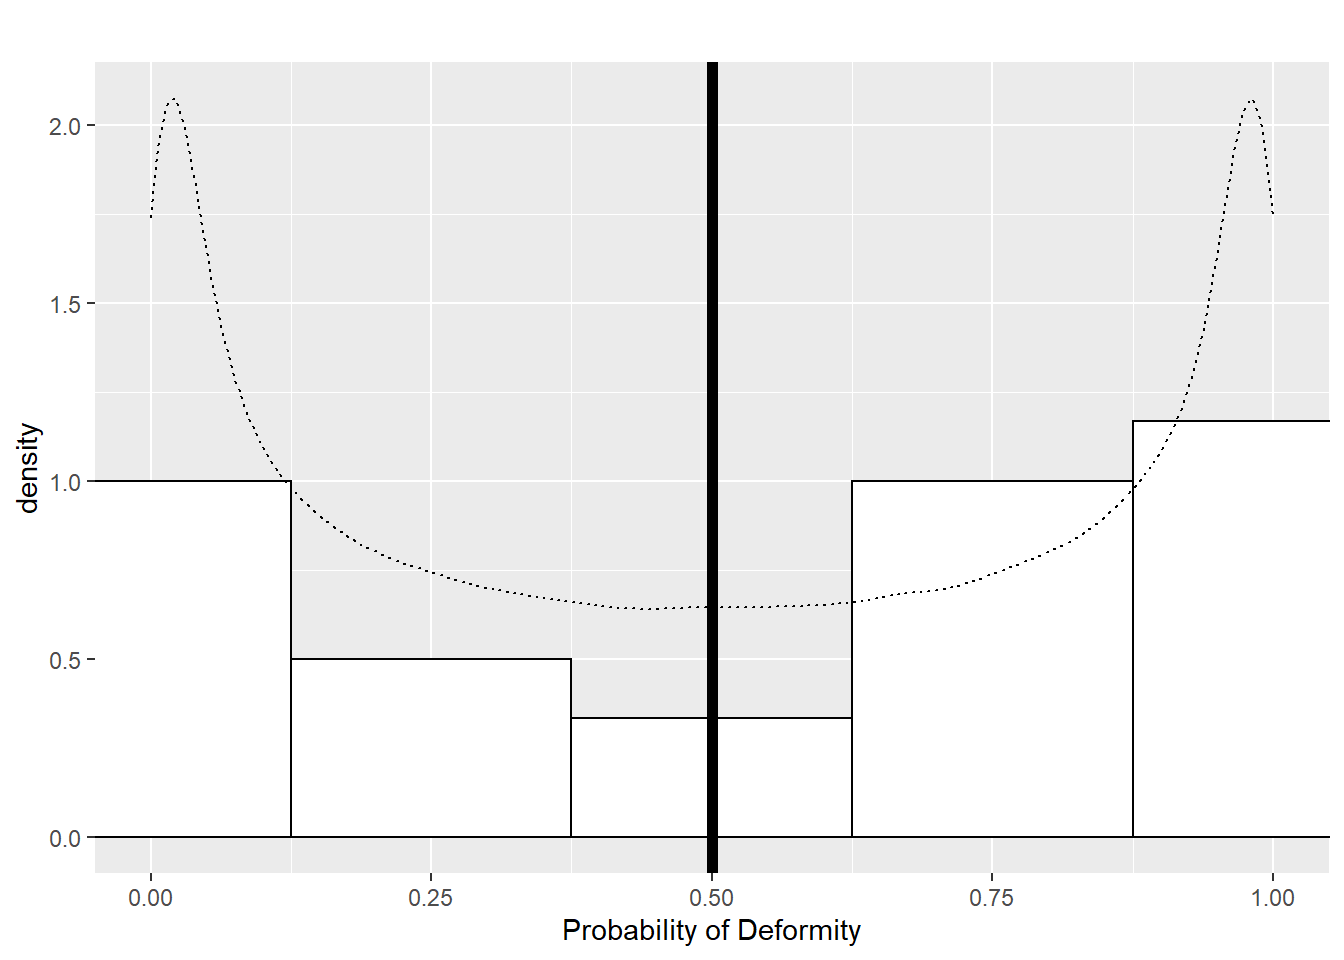
\includegraphics[width=0.6\linewidth]{bookdown-bysh_files/figure-latex/scenario1ProbabilityPlot-1} 

}

\caption{Dam Probabilities in Scenario 1}\label{fig:scenario1ProbabilityPlot}
\end{figure}

\begin{figure}

{\centering 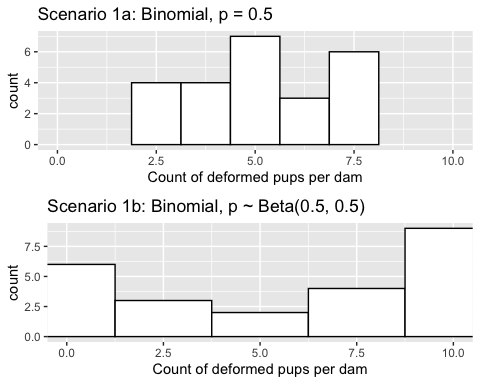
\includegraphics[width=0.6\linewidth]{bookdown-bysh_files/figure-latex/scenario1Plot-1} 

}

\caption{Counts of deformed pups per dam under Scenarios 1a and 1b}\label{fig:scenario1Plot}
\end{figure}

\vspace{5mm}

\textbf{Thought Questions}

\begin{enumerate}
\def\labelenumi{\arabic{enumi}.}
\item
  Will the counts of deformed pups for dams in Scenario 1a behave like a binomial distribution with \(n=10\) and \(p=0.5\) (that is, like counting heads in 10 flips of a fair coin)? Why or why not?
\item
  Will the counts of deformed pups for dams in Scenario 1b behave like a binomial distribution with \(n=10\) and \(p=0.5\) (that is, like counting heads in 10 flips of a fair coin)? If not, extend the coin flipping analogy to Scenario 1b.
\item
  Is Scenario 1b realistic? Why might some dams have higher probabilities than others?
\end{enumerate}

If we were to model the number of deformed pups per dam in Scenario 1a, we could ignore the potential of a dam effect (since all dams behave the same) and proceed with regular binomial regression as in Chapter \ref{ch-logreg}. Since we have no predictors, we would start with the model:

\begin{equation*}
  \log \bigg( \frac{\hat{p}}{1-\hat{p}} \bigg) = \hat{\beta}_0, \textrm{ where } \hat{\beta}_0 = 0.067
\end{equation*}
which produces an estimated odds of deformity \(\widehat{p}/(1-\widehat{p}) = e^{0.067} = 1.069\) and estimated probability \(\widehat{p} = 0.517\). Creating 95\% confidence intervals using a profile likelihood approach, we get:



\[
\begin{alignedat}{2}
  &\textrm{95\% CI for } p/(1-p) &&= (0.830, 1.378) \\
  &\textrm{95\% CI for } p       &&= (0.454, 0.579)
\end{alignedat}
\]

However, we can account for potential overdispersion \index{overdispersion} with a \textbf{quasibinomial model} \index{quasibinomial}, just as we did in Section \ref{sec-logOverdispersion}, in case the observed variance is larger than the variance under a binomial model. Quasibinomial regression yields the same estimate for \(\beta_0\) as the binomial regression model (\(\hat{\beta}_0 = 0.067\)), but we now have overdispersion paramater \(\widehat{\phi} = 0.894\). This gives us the following 95\% profile likelihood-based confidence intervals:

\[
\begin{alignedat}{2}
  &\textrm{95\% CI for } p/(1-p) &&= (0.841, 1.359) \\
  &\textrm{95\% CI for } p       &&= (0.457, 0.576)
\end{alignedat}
\]

Turning to Scenario 1b, where each dam has a unique probability of producing a pup with a deformity based on a beta distribution, we can fit binomial and quasibinomial models as well.

A binomial model gives regression equation

\begin{equation*}
  \log\bigg(\frac{\hat{p}}{1-\hat{p}}\bigg) = 0.268,
\end{equation*}
with associated profile likelihood 95\% confidence intervals:

\[
\begin{alignedat}{2}
  &\textrm{95\% CI for } p/(1-p) &&= (1.014, 1.691) \\
  &\textrm{95\% CI for } p       &&= (0.504, 0.628)
\end{alignedat}
\]

We could compare this to a quasibinomial model. With overdispersion paramater \(\widehat{\phi} = 6.858\), we now have profile likelihood-based intervals:

\[
\begin{alignedat}{2}
  &\textrm{95\% CI for } p/(1-p) &&= (0.673, 2.594) \\
  &\textrm{95\% CI for } p       &&= (0.402, 0.722)
\end{alignedat}
\]

\vspace{5mm}

\textbf{Thought Questions}

\begin{enumerate}
\def\labelenumi{\arabic{enumi}.}
\setcounter{enumi}{3}
\item
  Describe how the quasibinomial analysis of Scenario 1b differs from the binomial analysis of the same simulated data. Refer to Table \ref{tab:simulationTableCh7} when answering this question; you will need to run the R code in the R markdown file for this chapter to completely fill out the table. Do confidence intervals contain the true model parameters?
\item
  Why are differences between quasibinomial and binomial models of Scenario 1a less noticeable than the differences in Scenario 1b?
\end{enumerate}

\hypertarget{scenario-2-dose-effect}{%
\section{Scenario 2: Dose effect}\label{scenario-2-dose-effect}}

In Scenario 1, each dam's probability of producing a deformed pup was independent of their dosage of the teratogen. In Scenario 2 we allow for a dose effect. To recall, in this hypothetical experiment we have 24 total dams evenly split into 4 groups recieving either no dose (coded as \texttt{dose\ =\ 0} mg), a low dose (\texttt{dose\ =\ 1}), a medium dose (\texttt{dose\ =\ 2}), or a high dose (\texttt{dose\ =\ 3}) of the teratogen.

We will suppose that true probability that a dam's pup has a deformity is related to the dose the dam received through this model:

\[ \log \bigg(\frac{p}{1-p} \bigg) = -2 + 1.33\; \textrm{dose} \]
That is, we assume that the log odds of a deformity is linearly related to dose through the equation above, and the odds of a deformity are 3.79 times greater (\(e^{1.33}\)) for each 1mg increase in dose.

In Scenario 2a, a dam who received a dose of \(x\) would have probability

\[p = P(\textrm{deformity}\mid \textrm{dose} = x) = e^{-2+1.33x}/(1+e^{-2+1.33x}). \]
Thus, dams who received doses of 0, 1, 2, and 3 mg would have probabilities 0.12, 0.34, 0.66, and 0.88, respectively, under Scenario 2a.

In Scenario 2b, each dam who received a dose of \(x\) has probability of deformity randomly chosen from a beta distribution where \(\alpha = 2p/(1-p)\) and \(\beta = 2\). These beta distribution parameters ensure that, on average, dams with a dose \(x\) in Scenario 2b have the same probability of a deformed pup as dams with dose \(x\) in Scenario 2a. For example, dams receiving the 1mg dosage under Scenario 2b would have probabilities following a beta distribution with \(\alpha = 2(0.34)/(1-0.34) = 1.03\) and \(\beta = 2\), which has mean \(\frac{\alpha}{\alpha + \beta}=0.34\). The big difference is that \emph{all} dams receiving the 1mg dosage in Scenario 2a have probability 0.34 of a deformed pup, whereas dams receiving the 1mg dosage in Scenario 2b each have a unique probability of a deformed pup, but those probabilities average out to 0.34.

Figure \ref{fig:scenario2bPlot} displays histograms for each dosage group of each dam's probability of producing deformed pups under Scenario 2b as well as theoretical distributions of probabilities. A vertical line is displayed at each hypothetical distribution's mean; the vertical line represents the fixed probability of a deformed pup for all dams under Scenario 2a.

\begin{Shaded}
\begin{Highlighting}[]
\KeywordTok{set.seed}\NormalTok{(}\DecValTok{1}\NormalTok{)}

\NormalTok{dose <-}\StringTok{ }\KeywordTok{c}\NormalTok{(}\KeywordTok{rep}\NormalTok{(}\DecValTok{0}\NormalTok{,}\DecValTok{6}\NormalTok{),}\KeywordTok{rep}\NormalTok{(}\DecValTok{1}\NormalTok{,}\DecValTok{6}\NormalTok{),}\KeywordTok{rep}\NormalTok{(}\DecValTok{2}\NormalTok{,}\DecValTok{6}\NormalTok{),}\KeywordTok{rep}\NormalTok{(}\DecValTok{3}\NormalTok{,}\DecValTok{6}\NormalTok{))}

\NormalTok{pi_2a <-}\StringTok{ }\KeywordTok{exp}\NormalTok{(}\OperatorTok{-}\DecValTok{2}\OperatorTok{+}\DecValTok{4}\OperatorTok{/}\DecValTok{3}\OperatorTok{*}\NormalTok{dose)}\OperatorTok{/}\NormalTok{(}\DecValTok{1}\OperatorTok{+}\KeywordTok{exp}\NormalTok{(}\OperatorTok{-}\DecValTok{2}\OperatorTok{+}\DecValTok{4}\OperatorTok{/}\DecValTok{3}\OperatorTok{*}\NormalTok{dose))}
\NormalTok{count_2a <-}\StringTok{ }\KeywordTok{rbinom}\NormalTok{(}\DecValTok{24}\NormalTok{, }\DecValTok{10}\NormalTok{, pi_2a)}

\NormalTok{b <-}\StringTok{ }\DecValTok{2}
\NormalTok{a <-}\StringTok{ }\NormalTok{b}\OperatorTok{*}\NormalTok{pi_2a }\OperatorTok{/}\StringTok{ }\NormalTok{(}\DecValTok{1}\OperatorTok{-}\NormalTok{pi_2a)}
\NormalTok{pi_2b <-}\StringTok{ }\KeywordTok{rbeta}\NormalTok{(}\DecValTok{24}\NormalTok{, a, b)}
\NormalTok{count_2b <-}\StringTok{ }\KeywordTok{rbinom}\NormalTok{(}\DecValTok{24}\NormalTok{, }\DecValTok{10}\NormalTok{, pi_2b)  }
\end{Highlighting}
\end{Shaded}

\begin{figure}

{\centering 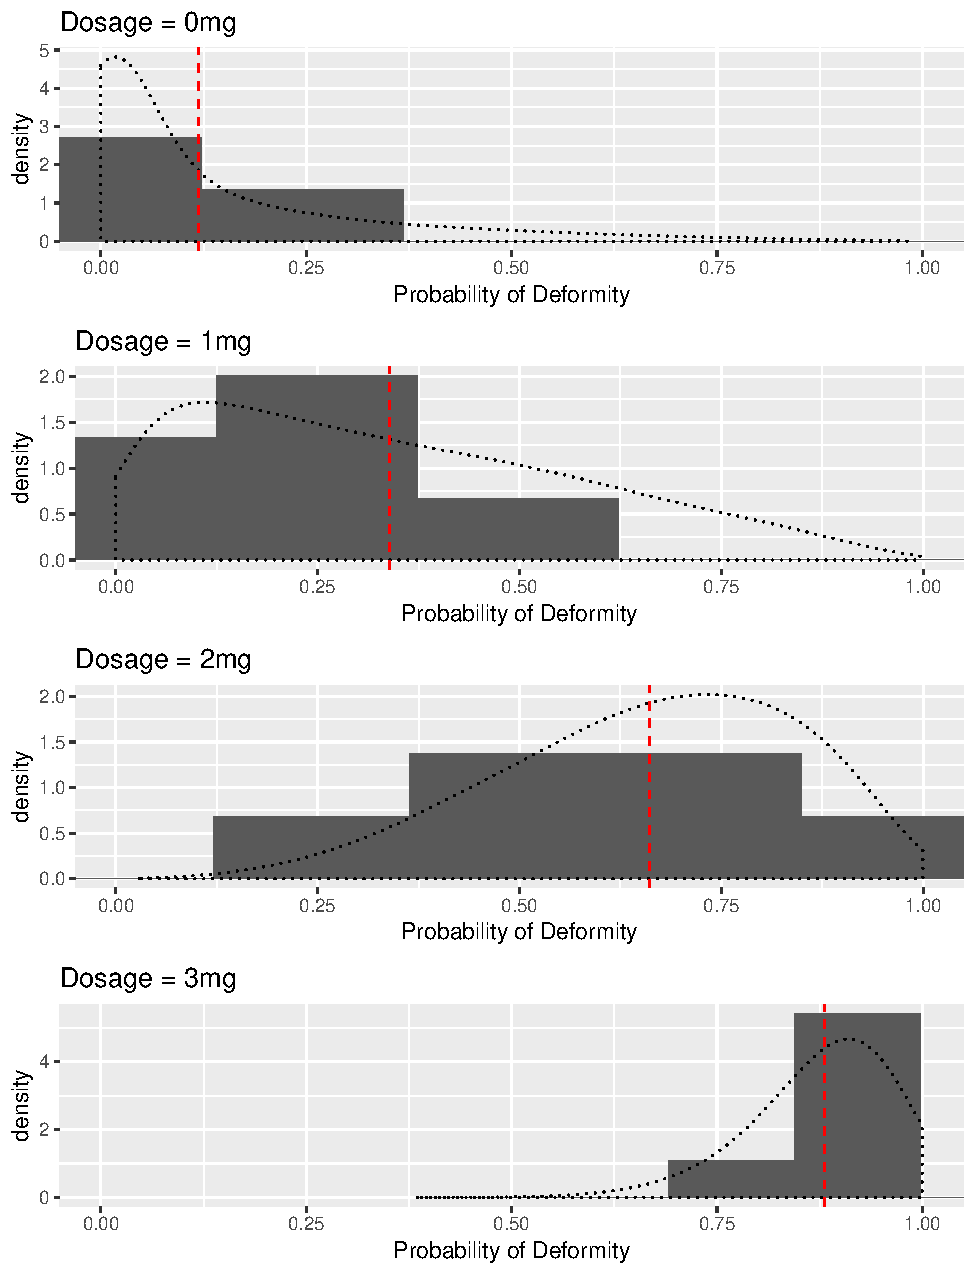
\includegraphics[width=0.6\linewidth]{bookdown-bysh_files/figure-latex/scenario2bPlot-1} 

}

\caption{Observed (histograms) and theoretical (density curves) distributions of dams' probabilities of producing deformed pups by dose group in Scenario 2b.  The red vertical line represents the fixed probability of a deformed pup by dose group in Scenario 2a.}\label{fig:scenario2bPlot}
\end{figure}

\begin{table}

\caption{\label{tab:scenario2Tab}Summary Statistics of Scenario 2 by Dose}
\centering
\resizebox{\linewidth}{!}{
\begin{tabular}[t]{rrr>{\raggedleft\arraybackslash}p{1cm}>{\raggedleft\arraybackslash}p{1cm}rr>{\raggedleft\arraybackslash}p{1cm}>{\raggedleft\arraybackslash}p{1cm}}
\toprule
\multicolumn{1}{c}{ } & \multicolumn{4}{c}{Scenario 2a} & \multicolumn{4}{c}{Scenario 2b} \\
\cmidrule(l{3pt}r{3pt}){2-5} \cmidrule(l{3pt}r{3pt}){6-9}
Dosage & Mean p & SD p & Mean Count & SD Count & Mean p & SD p & Mean Count & SD Count\\
\midrule
0 & 0.119 & 0 & 1.333 & 1.366 & 0.061 & 0.069 & 0.500 & 0.837\\
1 & 0.339 & 0 & 3.167 & 1.835 & 0.239 & 0.208 & 3.500 & 2.881\\
2 & 0.661 & 0 & 5.833 & 1.472 & 0.615 & 0.195 & 5.833 & 1.941\\
3 & 0.881 & 0 & 8.833 & 1.169 & 0.872 & 0.079 & 8.833 & 1.169\\
\bottomrule
\end{tabular}}
\end{table}

\vspace{5mm}

\textbf{Thought Questions}

\begin{enumerate}
\def\labelenumi{\arabic{enumi}.}
\setcounter{enumi}{5}
\item
  Compare and contrast the probabilities associated with the 24 dams under Scenarios 1a and 1b to the probabilities under Scenarios 2a and 2b.
\item
  In Scenario 2a, dams produced 4.79 deformed pups on average, with standard deviation 3.20. Scenario 2b saw an average of 4.67 with standard deviation 3.58. Explain why comparisons by dose are more meaningful than these overall comparisons. You might refer to the results in Table \ref{tab:scenario2Tab}.
\item
  In Table \ref{tab:simulationTableCh7}, predict what you'll see in the column headed ``CI\_odds\_ratio''. Among the 4 entries: What can you say about the center and the width of the confidence intervals? Which will be similar and why? Which will be different and how?
\end{enumerate}

We first model Scenario 2a without adjusting for potential overdispersion. Binomial regression gives us the model:

\begin{equation}
  \log\bigg( \frac{\hat{p}}{1-\hat{p}} \bigg) = -2.02 + 1.26\;\textrm{dose}
  \label{eq:mod2aBinom}
\end{equation}
Equation \eqref{eq:mod2aBinom} has associated odds ratio corresponding to a 1mg dose increase of \(e^{\beta_1} = 3.54\) with 95\% profile likelihood confidence interval \((2.61, 4.96)\). We can be 95\% confident that odds of deformity are between 2.61 and 4.96 times higher for each 1 mg increase in dose.

Alternatively, we can use a quasibinomial model to account for any overdispersion in the binomial model. With \(\widehat{\phi} = 1.27\), we have the 95\% profile likelihood confidence interval for \(e^\beta_1\): \((2.51, 5.19)\).

Turning to Scenario 2b, where probabilities were different between dams recieving the same dosage, we have the binomial model

\begin{equation*}
  \log\bigg( \frac{\hat{p}}{1-\hat{p}} \bigg) = -2.41 + 1.46\;\textrm{dose}
\end{equation*}
Generating a 95\% confidence interval for \(e^{\beta_1}\), we have: \((3.09, 6.27)\).

If we use a quasibinomial model, we find overdispersion paramater \(\widehat{\phi} = 1.93\), yielding 95\% confidence interval for \(e^{\beta_1}\): \((2.74, 7.35)\).

\vspace{5mm}

\textbf{Thought Questions}

\begin{enumerate}
\def\labelenumi{\arabic{enumi}.}
\setcounter{enumi}{8}
\item
  Describe how the quasibinomial analysis of Scenario 2b differs from the binomial analysis of the same simulated data. Refer to Table \ref{tab:simulationTableCh7} when answering this question; you will need to run the R code in the R markdown file for this chapter to completely fill out the table. Do confidence intervals contain the true model parameters?
\item
  Why are differences between quasibinomial and binomial models of Scenario 2a less noticeable than the differences in Scenario 2b?
\item
  Why does Scenario 2b contain correlated data that we must account for, while Scenario 2a does not?
\end{enumerate}

\hypertarget{case-study-tree-growth}{%
\section{Case Study: Tree Growth}\label{case-study-tree-growth}}

A student research team at St.~Olaf College contributed to the efforts of biologist Kathy Shea to investigate a rich data set concerning forestation in the surrounding land. \citep{Eisinger2011} Here is a paragraph from the introduction to their project report:

\begin{quote}
Much of south-central Minnesota was comprised of maple-basswood forest prior to agricultural development and settlement. Currently, the forests that remain are highly fragmented and disturbed by human activities. Original land surveys describe the forest, also known as the Big Woods ecosystem, as dominated by elm, maple, oak, and basswood. In order to recover the loss of ecosystem services that forests provide, many new forested areas have been established through restoration.
\end{quote}

Tubes were placed on trees in some locations or \emph{transects} but not in others. One research question is whether tree growth in the first year is affected by the presence of tubes. This analysis has a structure similar to the dams and pups; the two study designs are depicted in Figure \ref{fig:DamsTreesStructure}.

\begin{figure}
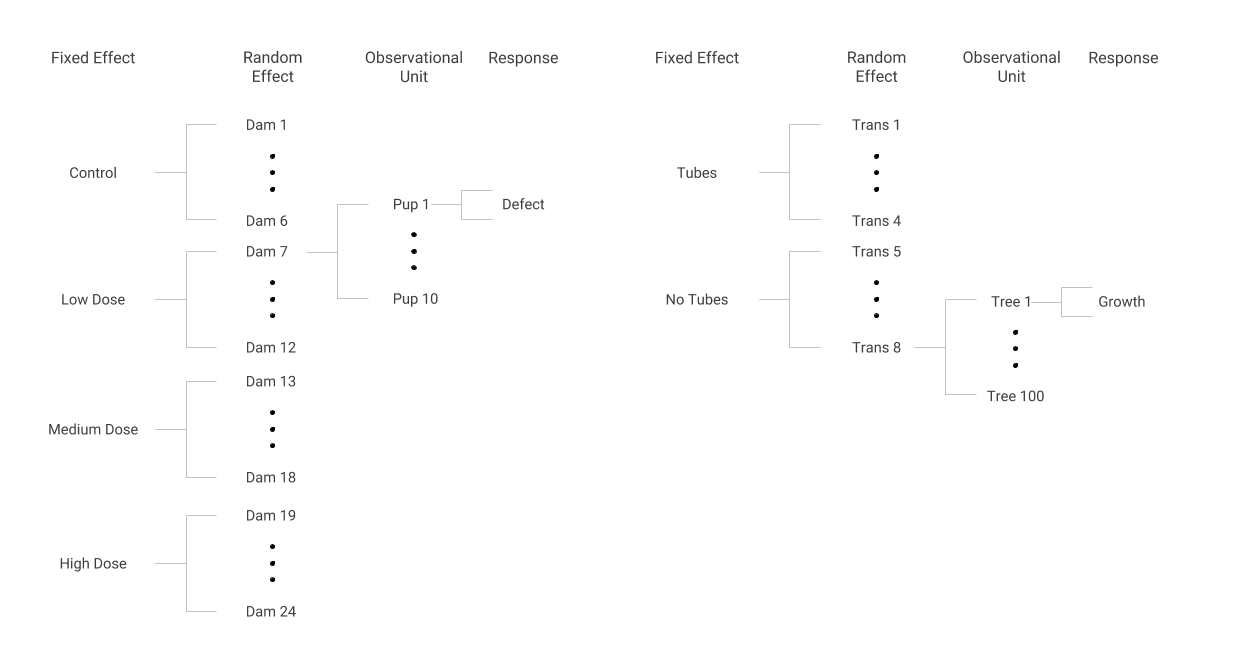
\includegraphics[width=0.8\linewidth]{data/DamsTreesStructure} \caption{Data structures in the Dams and Pups (left) and Tree Growth (right) case studies}\label{fig:DamsTreesStructure}
\end{figure}

Some transects were assigned to have tubes on all of their trees and other transects had no tubes on all of their trees, just as every dam assigned to a certain group received the same dose. Within a transect, each tree's first year of growth was measured, much like the presence or absence of a defect was noted for every pup within a dam. Although the response in the tree tube study is continuous (and somewhat normally distributed) rather than binary as in the dams and pups study, we can use methods to account for correlation of trees within a transect, just as we accounted for correlation of pups within dams.

\hypertarget{format-of-the-data-set}{%
\subsection{Format of the data set}\label{format-of-the-data-set}}

We will consider a subset of the full data set in \texttt{treetube.csv} for illustration purposes here: the 382 trees with heights recorded in both 1990 and 1991. Thus, we will consider the following variables:

\begin{itemize}
\tightlist
\item
  \texttt{id} = a unique identifier for each tree
\item
  \texttt{transect} = a unique identifier for each transect containing several trees
\item
  \texttt{species} = tree species
\item
  \texttt{tubes} = an indicator variable for the presence or absence of tubes for a given transect
\item
  \texttt{height91} = first year height for each tree in meters
\item
  \texttt{height90} = baseline height for each tree in meters
\item
  \texttt{growth\_yr1} = height91 - height90, in meters
\end{itemize}

A sample of 10 observations are displayed in Table \ref{tab:treeTubeTab}.

\begin{table}

\caption{\label{tab:treeTubeTab}A sample of 10 trees and their growth from 1990 to 1991}
\centering
\begin{tabular}[t]{rrlrrrr}
\toprule
id & transect & species & tubes & height91 & height90 & growth\_yr1\\
\midrule
398 & 14 & Black Walnut & 0 & 0.332 & 0.200 & 0.132\\
402 & 14 & Black Walnut & 0 & 0.354 & 0.330 & 0.024\\
450 & 18 & Black Walnut & 1 & 0.214 & 0.174 & 0.040\\
451 & 18 & Black Walnut & 1 & 0.342 & 0.289 & 0.053\\
453 & 18 & Black Walnut & 1 & 0.395 & 0.205 & 0.190\\
\addlinespace
458 & 18 & Black Walnut & 1 & 0.420 & 0.290 & 0.130\\
560 & 22 & Black Walnut & 0 & 0.400 & 0.295 & 0.105\\
564 & 22 & Black Walnut & 0 & 0.549 & 0.390 & 0.159\\
569 & 22 & Black Walnut & 0 & 0.340 & 0.270 & 0.070\\
571 & 22 & Black Walnut & 0 & 0.394 & 0.271 & 0.123\\
\bottomrule
\end{tabular}
\end{table}

This portion of the data indicates that the four trees in transect 18 have tubes, while the other six trees listed do not. The concern with this kind of data structure is that trees from the same transect may be more similar or correlated with one another in contrast to trees from other transects. This could be true for a variety of reasons: some transects may receive less sun than others, or irrigation of the soil may differ from transect to transect. These unmeasured but possibly influential factors may imply a correlation among trees within transects. In that case, we would not have independent pieces of information, so that the number of trees within a transect would overstate the amount of independent information. To prepare for an analysis of this potentially correlated data, we examine the sources of variability in first-year tree growth.

\hypertarget{sources-of-variability-1}{%
\subsection{Sources of variability}\label{sources-of-variability-1}}

First year tree growth may vary because of:

\textbf{Tube effects} A purpose of this analysis is to determine whether tubes affect first year tube growth. Differences in mean growth based on the presence or absence of tubes would be of interest to researchers, and they would be included in a publication for this analysis. For this reason, tube effects are referred to as \textbf{fixed effects}. This is analogous to the dose effect in the dams and pups example.

\textbf{Transect effects} For some of the factors previously mentioned such as sun exposure or water availability, first year growth may vary by transect. Knowing which specific transects produce greater growth is not of interest and would not appear in a publication of this study. These \textbf{random effects} are analogous to dam effects which were not of inherent interest, but which we nevertheless wished to account for.

\textbf{Tree-to-tree variability within transects} There is inherent variability in tree growth even when they are subject to the same transect and treatment effects. This variability remains unexplained in our model, although we will attempt to explain some of it with covariates such as species.

Data sets with this kind of structure are often referred to as \textbf{multilevel data} \index{multilevel data}, and the remaining chapters delve into models for multilevel data in gory detail. With a continuous response variable, we will actually add random effects for transects to a more traditional linear least squares regression model rather than estimate an overdispersion parameter as with a binary response. Either way, if observations are really correlated, proper accounting will lead to larger standard errors for model coefficients and larger (but more appropriate) p-values for testing the significance of those coefficients.

\hypertarget{analysis-preview-accounting-for-correlation-within-transect}{%
\subsection{Analysis preview: accounting for correlation within transect}\label{analysis-preview-accounting-for-correlation-within-transect}}

Attempting to model the effects of tubes on tree growth, we could use LLSR which yields the model:

\begin{equation*}
  \hat{\textrm{Growth}} = 0.106 - 0.040\; \textrm{Tube}
\end{equation*}

\begin{Shaded}
\begin{Highlighting}[]
\NormalTok{tube_linear <-}\StringTok{ }\KeywordTok{lm}\NormalTok{(growth_yr1 }\OperatorTok{~}\StringTok{ }\NormalTok{tubes, }\DataTypeTok{data =}\NormalTok{ treetubes_yr1)}
\end{Highlighting}
\end{Shaded}

\begin{verbatim}
##             Estimate Std. Error t value  Pr(>|t|)
## (Intercept)  0.10585   0.005665  18.685 9.931e-56
## tubes       -0.04013   0.041848  -0.959 3.382e-01
\end{verbatim}

\begin{verbatim}
##  R squared =  0.002414 
##  Residual standard error =  0.1097
\end{verbatim}

However, the LLSR model assumes that all observations are independent, including trees in the same transect. One way to account for potential correlation is to estimate an additional parameter for the transect-to-transect variance. In other words, we are allowing for a random effect that each transect contributes to the overall variability. The multilevel model below does just that.

\begin{Shaded}
\begin{Highlighting}[]
\NormalTok{tube_multi1 <-}\StringTok{ }\KeywordTok{lmer}\NormalTok{(growth_yr1 }\OperatorTok{~}\StringTok{ }\NormalTok{tubes }\OperatorTok{+}\StringTok{ }\NormalTok{(}\DecValTok{1}\OperatorTok{|}\NormalTok{transect), }
                    \DataTypeTok{data =}\NormalTok{ treetubes_yr1)}
\end{Highlighting}
\end{Shaded}

\begin{verbatim}
##             Estimate Std. Error t value
## (Intercept)  0.10636    0.01329   8.005
## tubes       -0.04065    0.05165  -0.787
\end{verbatim}

\begin{verbatim}
##  Groups   Name        Variance Std.Dev.
##  transect (Intercept) 0.00084  0.029   
##  Residual             0.01155  0.107
\end{verbatim}

Like we saw in the case of the binary outcomes, the standard error for the coefficients is larger when we take correlation into account. The t-statistic for tubes is smaller, reducing our enthusisam for the tubes effect. This conservative approach occurs because the observations within a transect are correlated and therefore not independent as assumed in the naive model. We will study these models in depth in the remaining chapters.

\hypertarget{summary-1}{%
\section{Summary}\label{summary-1}}

The most important idea from this chapter is that structures of data sets may imply that outcomes are correlated. Correlated outcomes provide less information than independent outcomes, resulting in effective sample sizes that are less than the total number of observations. Neglecting to take into account correlation may lead to underestimating standard errors of coefficients, overstating significance and precision. Correlation is likely and should be accounted for if basic observational units (e.g., pups, trees) are aggregated in ways that would lead us to expect units within groups to be similar.

We have mentioned two ways to account for correlation: incorporate a dispersion parameter or include random effects. In the following chapters we will primarily focus on models with random effects. In fact, there are even more ways to account for correlation, including inflating the variance using Huber-White estimators (aka Sandwich estimators), and producing corrected variances using bootstrapping. These are beyond the scope of this text.

\hypertarget{exercises-3}{%
\section{Exercises}\label{exercises-3}}

\hypertarget{conceptual-exercises-1}{%
\subsection{Conceptual Exercises}\label{conceptual-exercises-1}}

\begin{enumerate}
\def\labelenumi{\arabic{enumi}.}
\tightlist
\item
  \textbf{Examples with Correlated Data} For each of the following studies:

  \begin{itemize}
  \tightlist
  \item
    Identify the most basic observational units
  \item
    Identify the grouping units (could be multiple levels of grouping)
  \item
    State the response(s) measured and variable type (normal, binary, Poisson, etc.)
  \item
    Write a sentence describing the within-group correlation.
  \item
    Identify fixed and random effects
  \end{itemize}
\end{enumerate}

\begin{enumerate}
\def\labelenumi{\alph{enumi}.}
\item
  \emph{Nurse Stress Study.} Four wards were randomly selected at each of 25 hospitals and randomly assigned to offer a stress reduction program for nurses on the ward or to serve as a control. At the conclusion of the study period, a random sample of 10 nurses from each ward completed a test to measure job-related stress. Factors assumed to be related include nurse experience, age, hospital size and type of ward.
\item
  \emph{Epilepsy Study.} Researchers conducted a randomized controlled study where patients were randomly assigned to either an anti-epileptic drug or a placebo. For each patient, the number of seizures at baseline was measured over a 2 week period. For four consecutive visits the number of seizures were determined over the past 2 week period. Patient age and sex along with visit number were recorded.
\item
  \emph{Cockroaches!} For a study of cockroach infestation, traps were set up in the kitchen, bathroom, and bedroom in a random sample of 100 New York City apartments. The goal is to estimate cockroach infestation levels given tenant income and age of the building.
\item
  \emph{Prairie Restoration.} Researchers at a small Midwestern college decided to experimentally explore the underlying causes of variation in soil reconstruction projects in order to make future projects more effective. Introductory ecology classes were organized to collect weekly data on plants in pots containing soil samples. Data will be examined to compare:

  \begin{itemize}
  \tightlist
  \item
    germination and growth of two species of prairie plants-----leadplants (\emph{Amorpha canescens}) and coneflowers (\emph{Ratibida pinnata})
  \item
    soil from a cultivated (agricultural) field, a natural prairie, and a restored (reconstructed) prairie.
  \item
    the effect of sterilization, since half of the sampled soil was sterilized to determine if rhizosphere differences were responsible for the observed variation.
  \end{itemize}
\item
  \emph{Radon in Minnesota.} Radon is a carcinogen -- a naturally occurring radioactive gas whose decay products are also radioactive -- known to cause lung cancer in high concentrations. The EPA sampled more than 80,000 homes across the US. Each house came from a randomly selected county and measurements were made on each level of each home. Uranium measurements at the county level were included to improve the radon estimates.
\item
  \emph{Teen Alcohol Use.} \citet{Curran1997} collected data on 82 adolescents at three time points starting at age 14 to assess factors that affect teen drinking behavior. Key variables in the data set \texttt{alcohol.csv} (source: \citet{Singer2003}) are as follows:

  \begin{itemize}
  \tightlist
  \item
    \texttt{id} = numerical identifier for subject
  \item
    \texttt{age} = 14, 15, or 16
  \item
    \texttt{coa} = 1 if the teen is a child of an alcoholic parent; 0 otherwise
  \item
    \texttt{male} = 1 if male; 0 if female
  \item
    \texttt{peer} = a measure of peer alcohol use, taken when each subject was 14. This is the square root of the sum of two 6-point items about the proportion of friends who drink occasionally or regularly.
  \item
    \texttt{alcuse} = the primary response. Four items---(a) drank beer or wine, (b) drank hard liquor, (c) 5 or more drinks in a row, and (d) got drunk---were each scored on an 8-point scale, from 0=''not at all'' to 7=''every day''. Then \texttt{alcuse} is the square root of the sum of these four items.
  \end{itemize}

  Primary research questions included:

  \begin{itemize}
  \tightlist
  \item
    do trajectories of alcohol use differ by parental alcoholism?
  \item
    do trajectories of alcohol use differ by peer alcohol use?
  \end{itemize}
\end{enumerate}

\begin{enumerate}
\def\labelenumi{\arabic{enumi}.}
\setcounter{enumi}{1}
\tightlist
\item
  \textbf{More dams and pups} Describe how to generalize the pup and dam example by allowing for different size litters.
\end{enumerate}

\hypertarget{guided-exercises-2}{%
\subsection{Guided Exercises}\label{guided-exercises-2}}

\begin{enumerate}
\def\labelenumi{\arabic{enumi}.}
\item
  \textbf{Exploring Beta Distributions.} In the Dams and Pups Case Study, we use the beta distribution to randomly select the probability that a dam produces a defective pup. While the beta distribution is described in Chapter \ref{ch-distthry}, it can be valuable to play with the parameters \(\alpha\) and \(\beta\) to see what distribution ranges and shapes are possible. Some basic R code for plotting a beta density curve can be found at the end of this problem.

  \begin{enumerate}
  \def\labelenumii{\alph{enumii}.}
  \tightlist
  \item
    What values do beta random variables take on?
  \item
    What do these values represent for the dams and pups simulation?
  \item
    Do the possible values depend on \(\alpha\) or \(\beta\)?
  \item
    What is a feature of the beta density when \(\alpha=\beta\)?
  \item
    What happens to the density when \(\alpha \neq \beta\)?
  \item
    How does the magnitude of \(\alpha\) or \(\beta\) affect the density?
  \item
    How does the difference between \(\alpha\) and \(\beta\) affect the density?
  \item
    If you wanted to simulate dams with mostly low probabilities of defects and a few with very high probabilities, how would you do it?
  \item
    If you wanted to simulate dams with mostly high probabilities of defects and a few with very low probabilities, how would you do it?
  \item
    If you wanted to simulate a population of dams where half of the probabilities of defects are very high and half are very low, how would you do it?
  \item
    How might you decide on values for \(\alpha\) and \(\beta\) if you have run a preliminary experiment and gathered data on the number of dams with deformed pups?
  \end{enumerate}
\end{enumerate}

\begin{Shaded}
\begin{Highlighting}[]
\CommentTok{# inputs for the beta distribution must be between 0 and 1}
\NormalTok{p <-}\StringTok{ }\KeywordTok{seq}\NormalTok{(}\DecValTok{0}\NormalTok{,}\DecValTok{1}\NormalTok{,}\DataTypeTok{by=}\NormalTok{.}\DecValTok{05}\NormalTok{)  }

\CommentTok{# To plot a beta density use dbeta; here I selected a=5, b=1}
\NormalTok{density <-}\StringTok{ }\KeywordTok{dbeta}\NormalTok{(p,}\DecValTok{5}\NormalTok{,}\DecValTok{1}\NormalTok{)}
\KeywordTok{plot}\NormalTok{(p, density, }\DataTypeTok{type =} \StringTok{"l"}\NormalTok{)}
\end{Highlighting}
\end{Shaded}

\begin{enumerate}
\def\labelenumi{\arabic{enumi}.}
\setcounter{enumi}{1}
\item
  \textbf{Dams and Pups (continued)}. Modify the dams and pups simulation in the following ways. In each case, produce plots and describe the results of your modified simulation.

  \begin{enumerate}
  \def\labelenumii{\alph{enumii}.}
  \tightlist
  \item
    Pick a different beta distribution for Scenario 1b.
  \item
    Center the beta distributions in Scenarios 1a and 1b somewhere other than 0.5.
  \item
    Repeat Scenario 2a with 3 doses and an underlying logistic model of your own choosing. Then create beta distributions as in Scenario 2b to match your 3 doses.
  \end{enumerate}
\end{enumerate}

\hypertarget{note-on-correlated-binary-outcomes}{%
\subsection{Note on Correlated Binary Outcomes}\label{note-on-correlated-binary-outcomes}}

The correlated binomial counts simulated in the Dams and Pups Case Study are in fact beta-binomial random variables like those simulated in the Guided Exercises from Chapter \ref{ch-distthry}. In fact, we could use the form of a beta-binomial pdf to model overdispersed binomial variables. Unlike the more generic form of accounting for correlation using dispersion parameter estimates, beta-binomial models are more specific and highly parameterized. This approach involves more assumptions but may also yield more information than the quasi-likelihood approach. If the beta-binomial model is incorrect, however, our results may be misleading. That said, the beta-binomial structure is quite flexible and conforms to many situations.

  \bibliography{bib/articles.bib,bib/books.bib,bib/misc.bib}

\backmatter
\printindex

\end{document}
